\chapter{Benchmarking}
\label{ch:chapter1}

\clearpage


\section{Datasets}

\subsection{Nault et al. 2022}

\begin{figure}[h]
    \centering
    \begin{subfigure}[t]{0.49\textwidth}
        \centering
        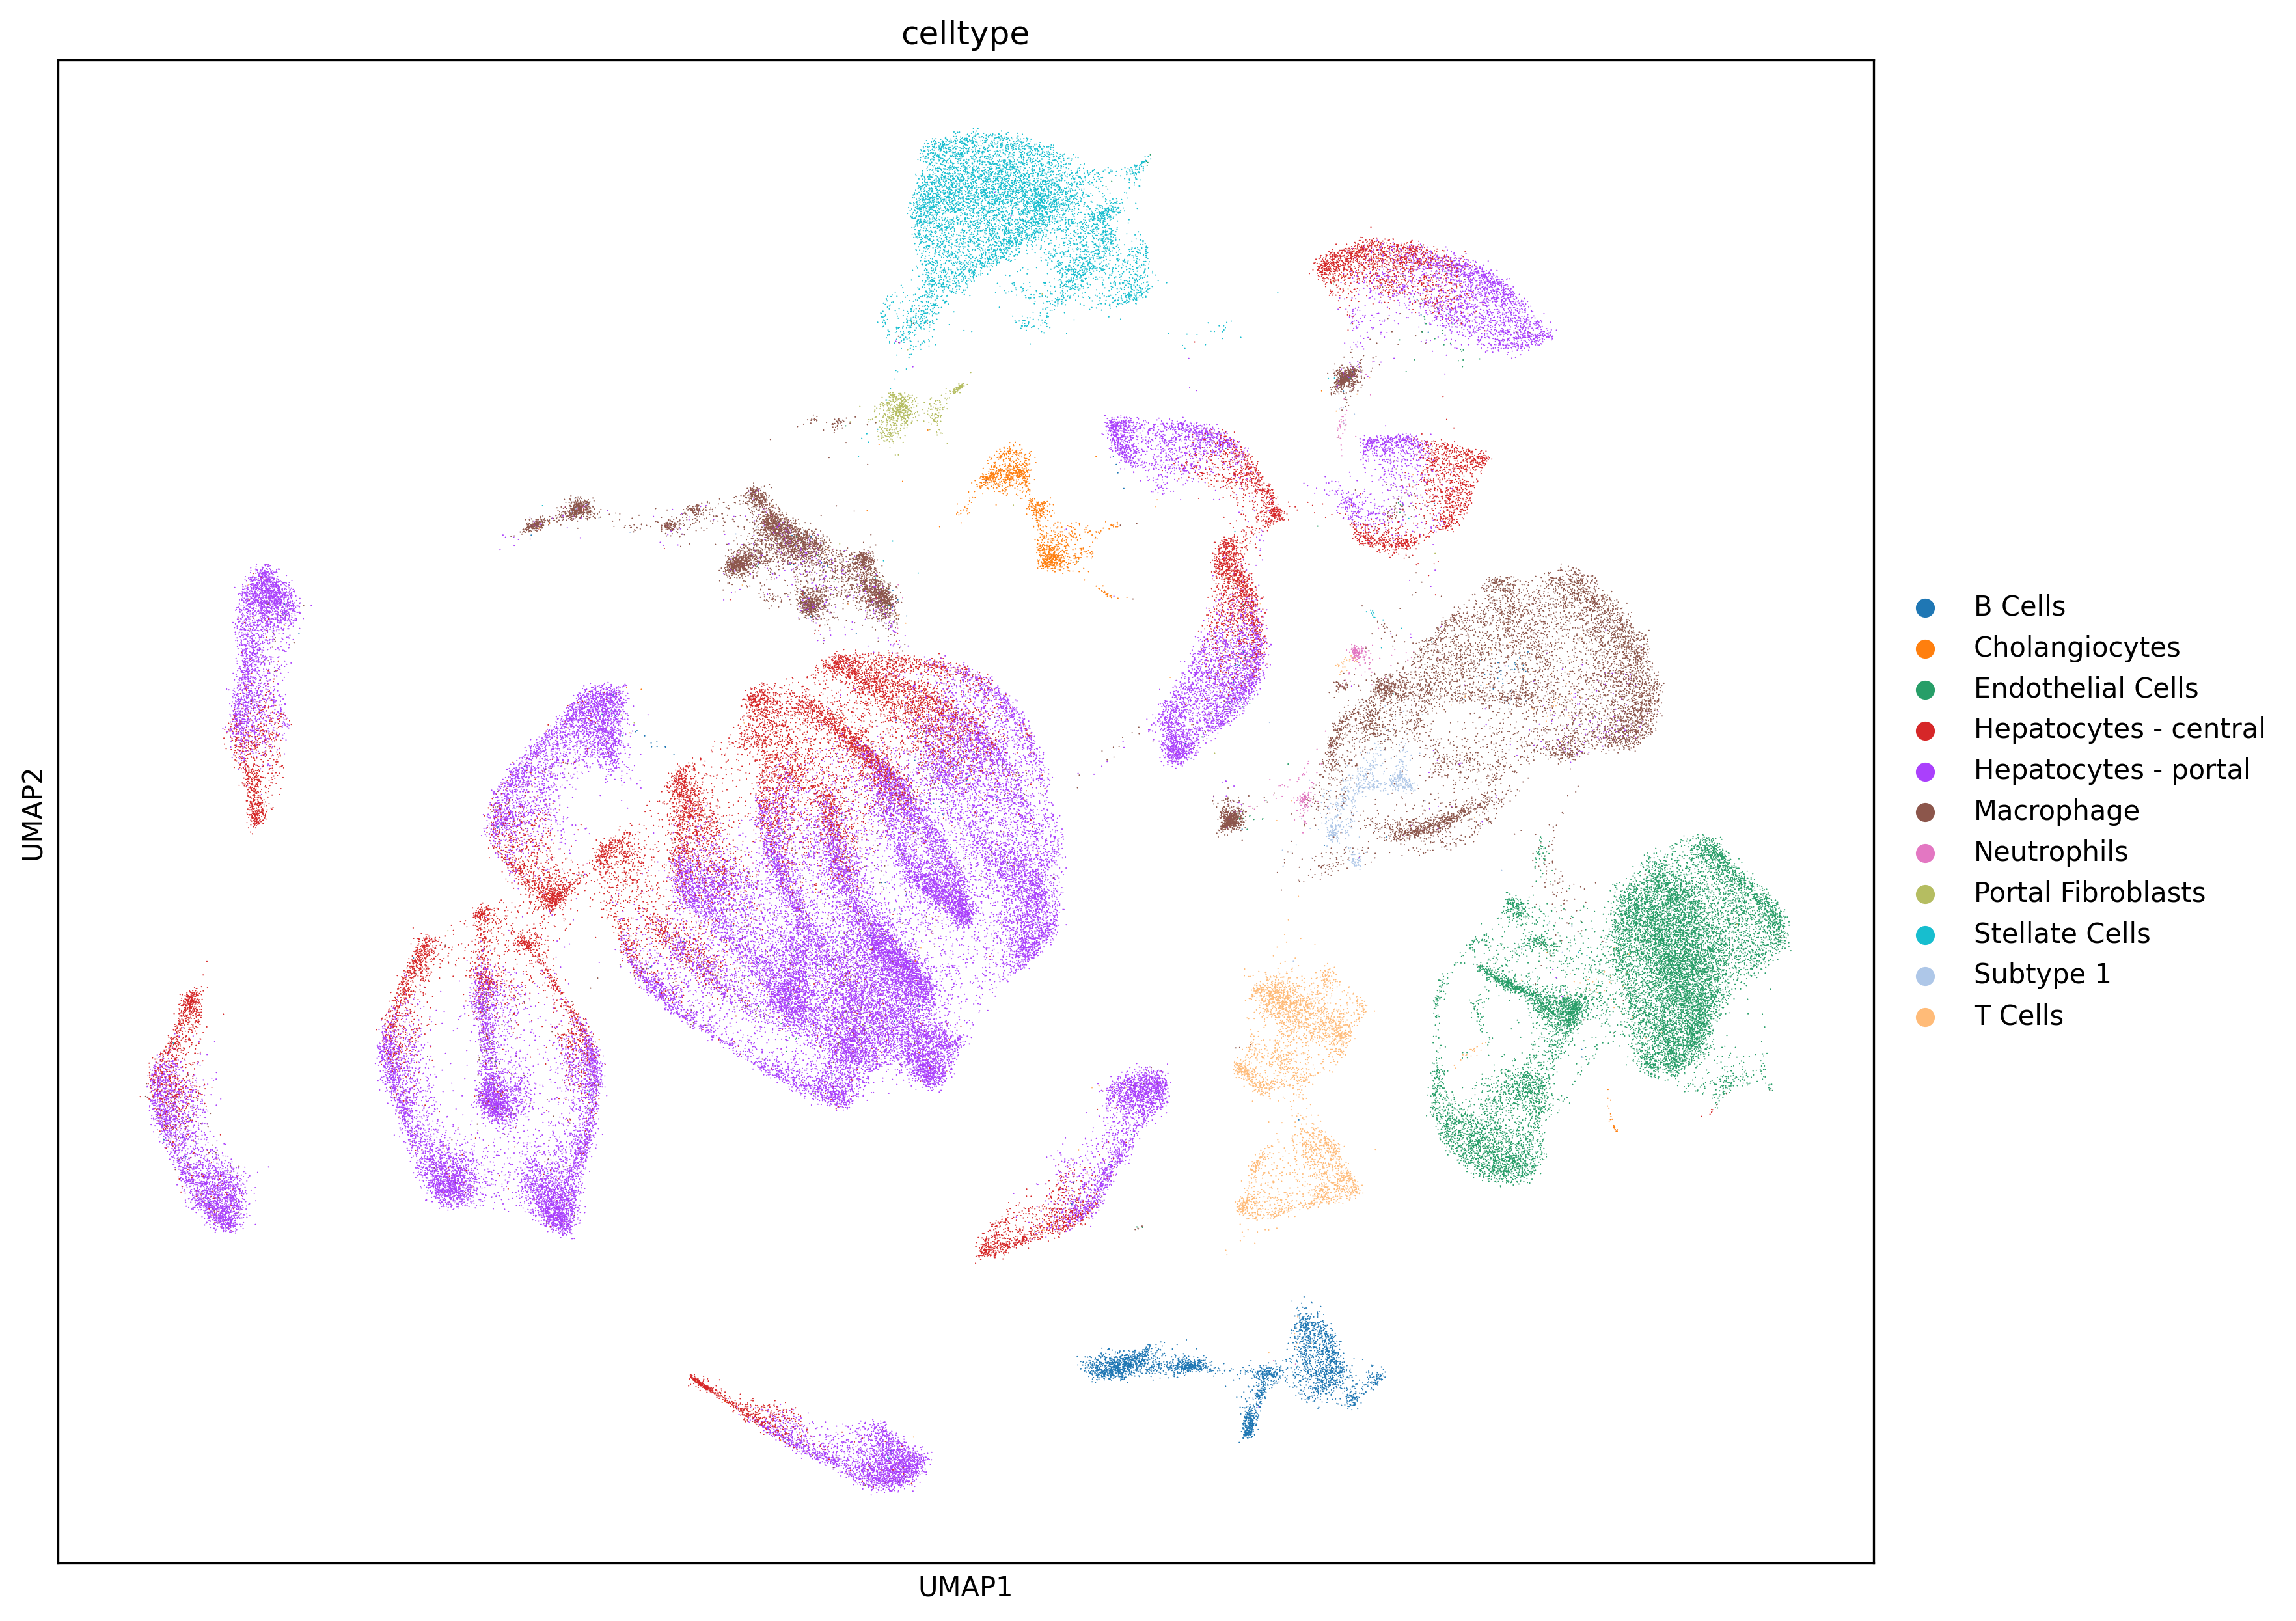
\includegraphics[width=.9\textwidth]{figures/nault_cell_umap.png}
        \caption{}
        \label{fig:figure1}.
    \end{subfigure}%
    \hfill
    \begin{subfigure}[t]{0.49\textwidth}
        \centering
        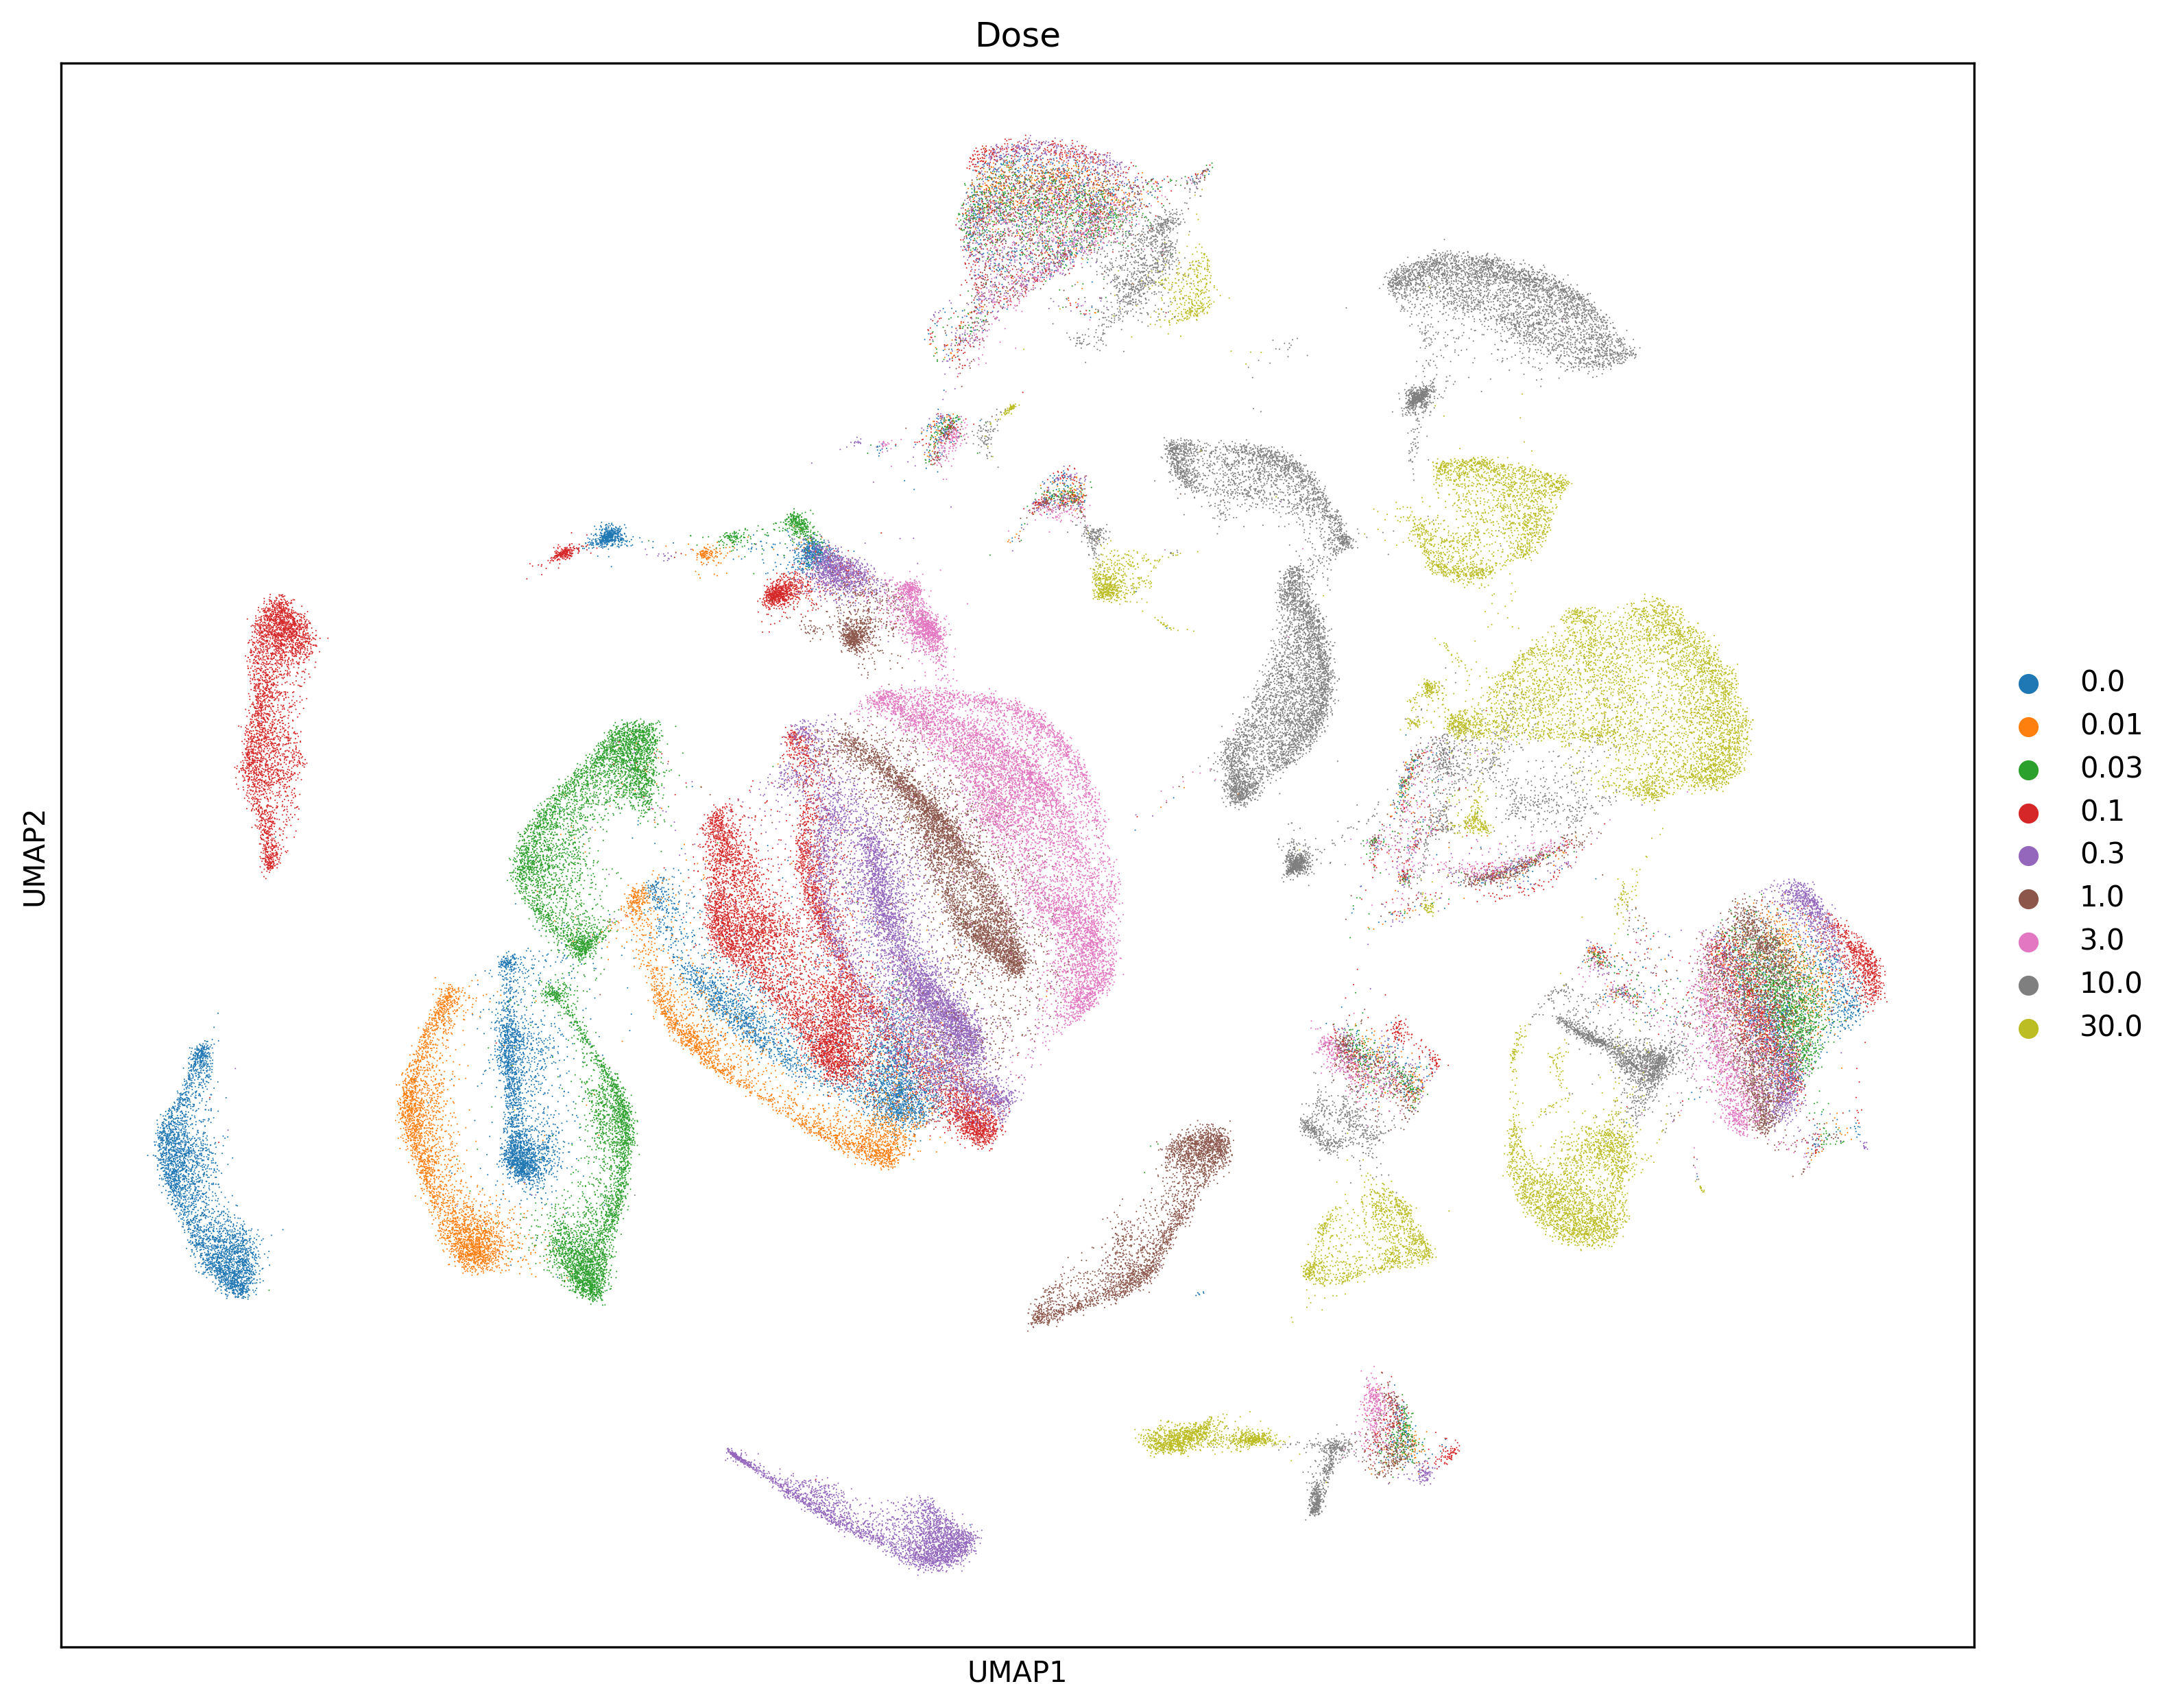
\includegraphics[width=.8\textwidth]{figures/nault_dose_umap.png}
        \caption{}
        \label{fig:figure2}
    \end{subfigure}%
    \hfill
    \begin{subfigure}[b]{\textwidth}
        \centering
        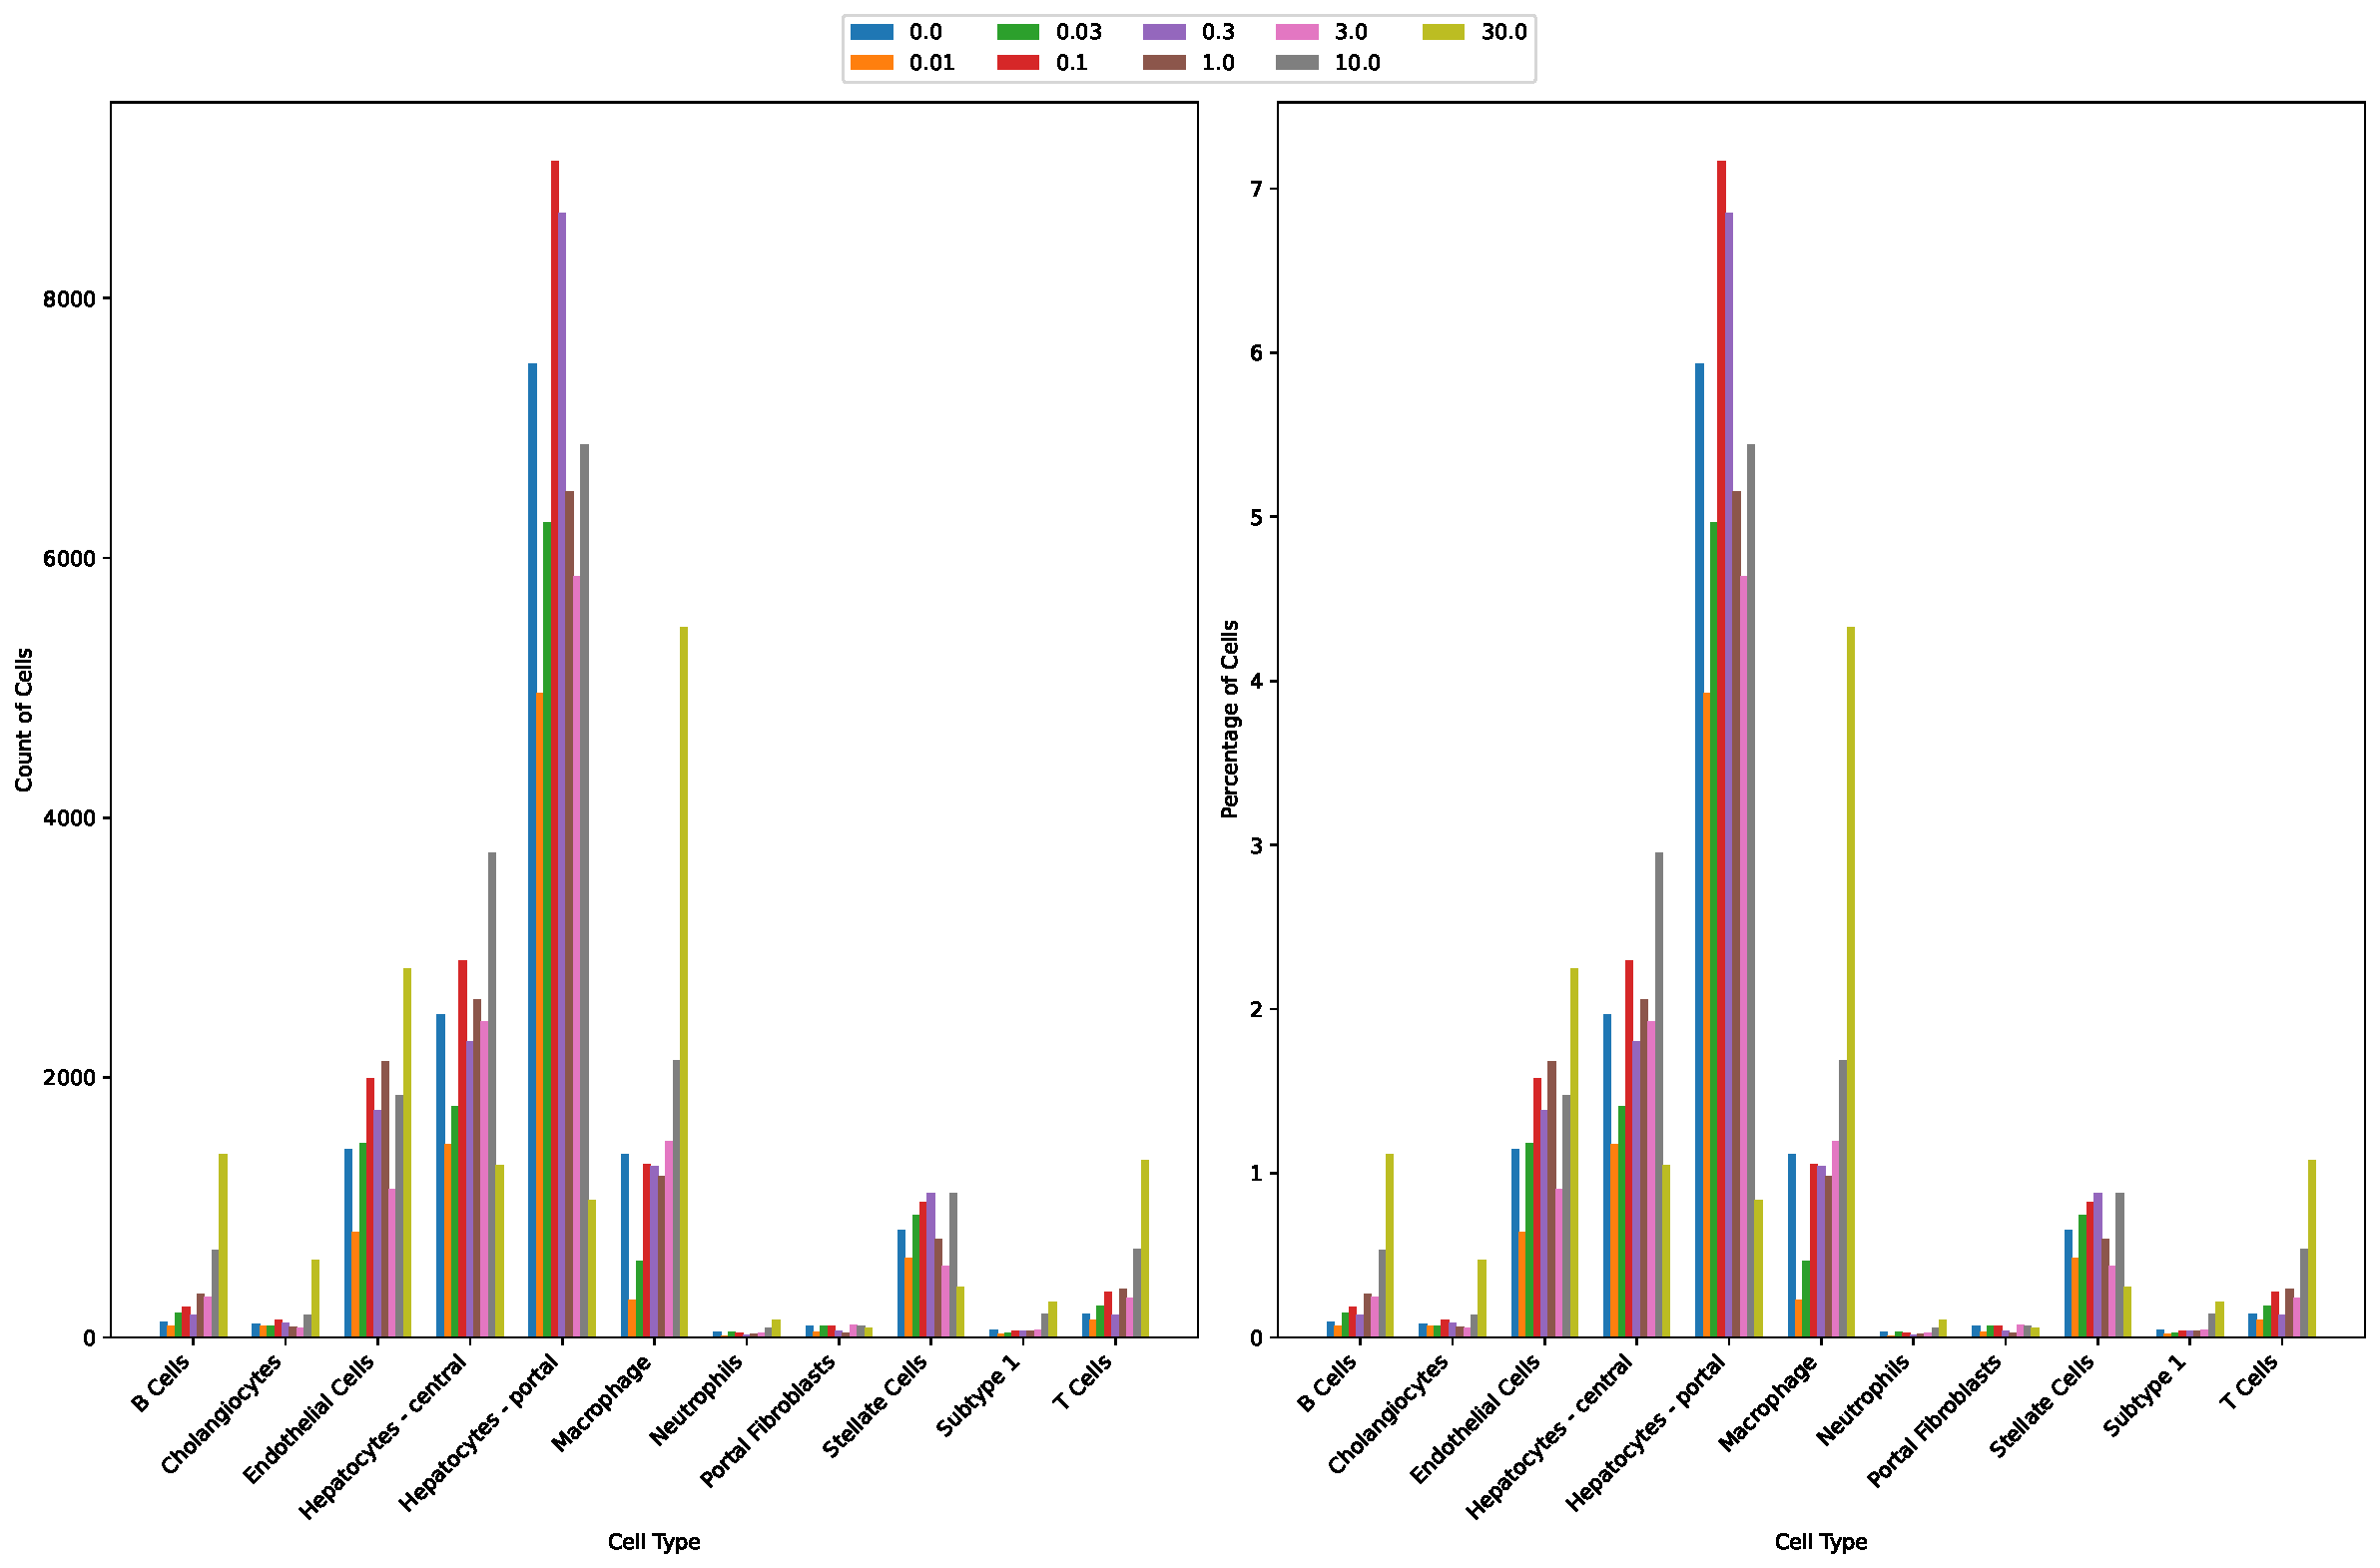
\includegraphics[width=.7\textwidth]{figures/nault_dosages_counts.pdf}
        \caption{}
        \label{fig:figure3}
    \end{subfigure}
    \hfill
    \begin{subfigure}[b]{\textwidth}
        \centering
        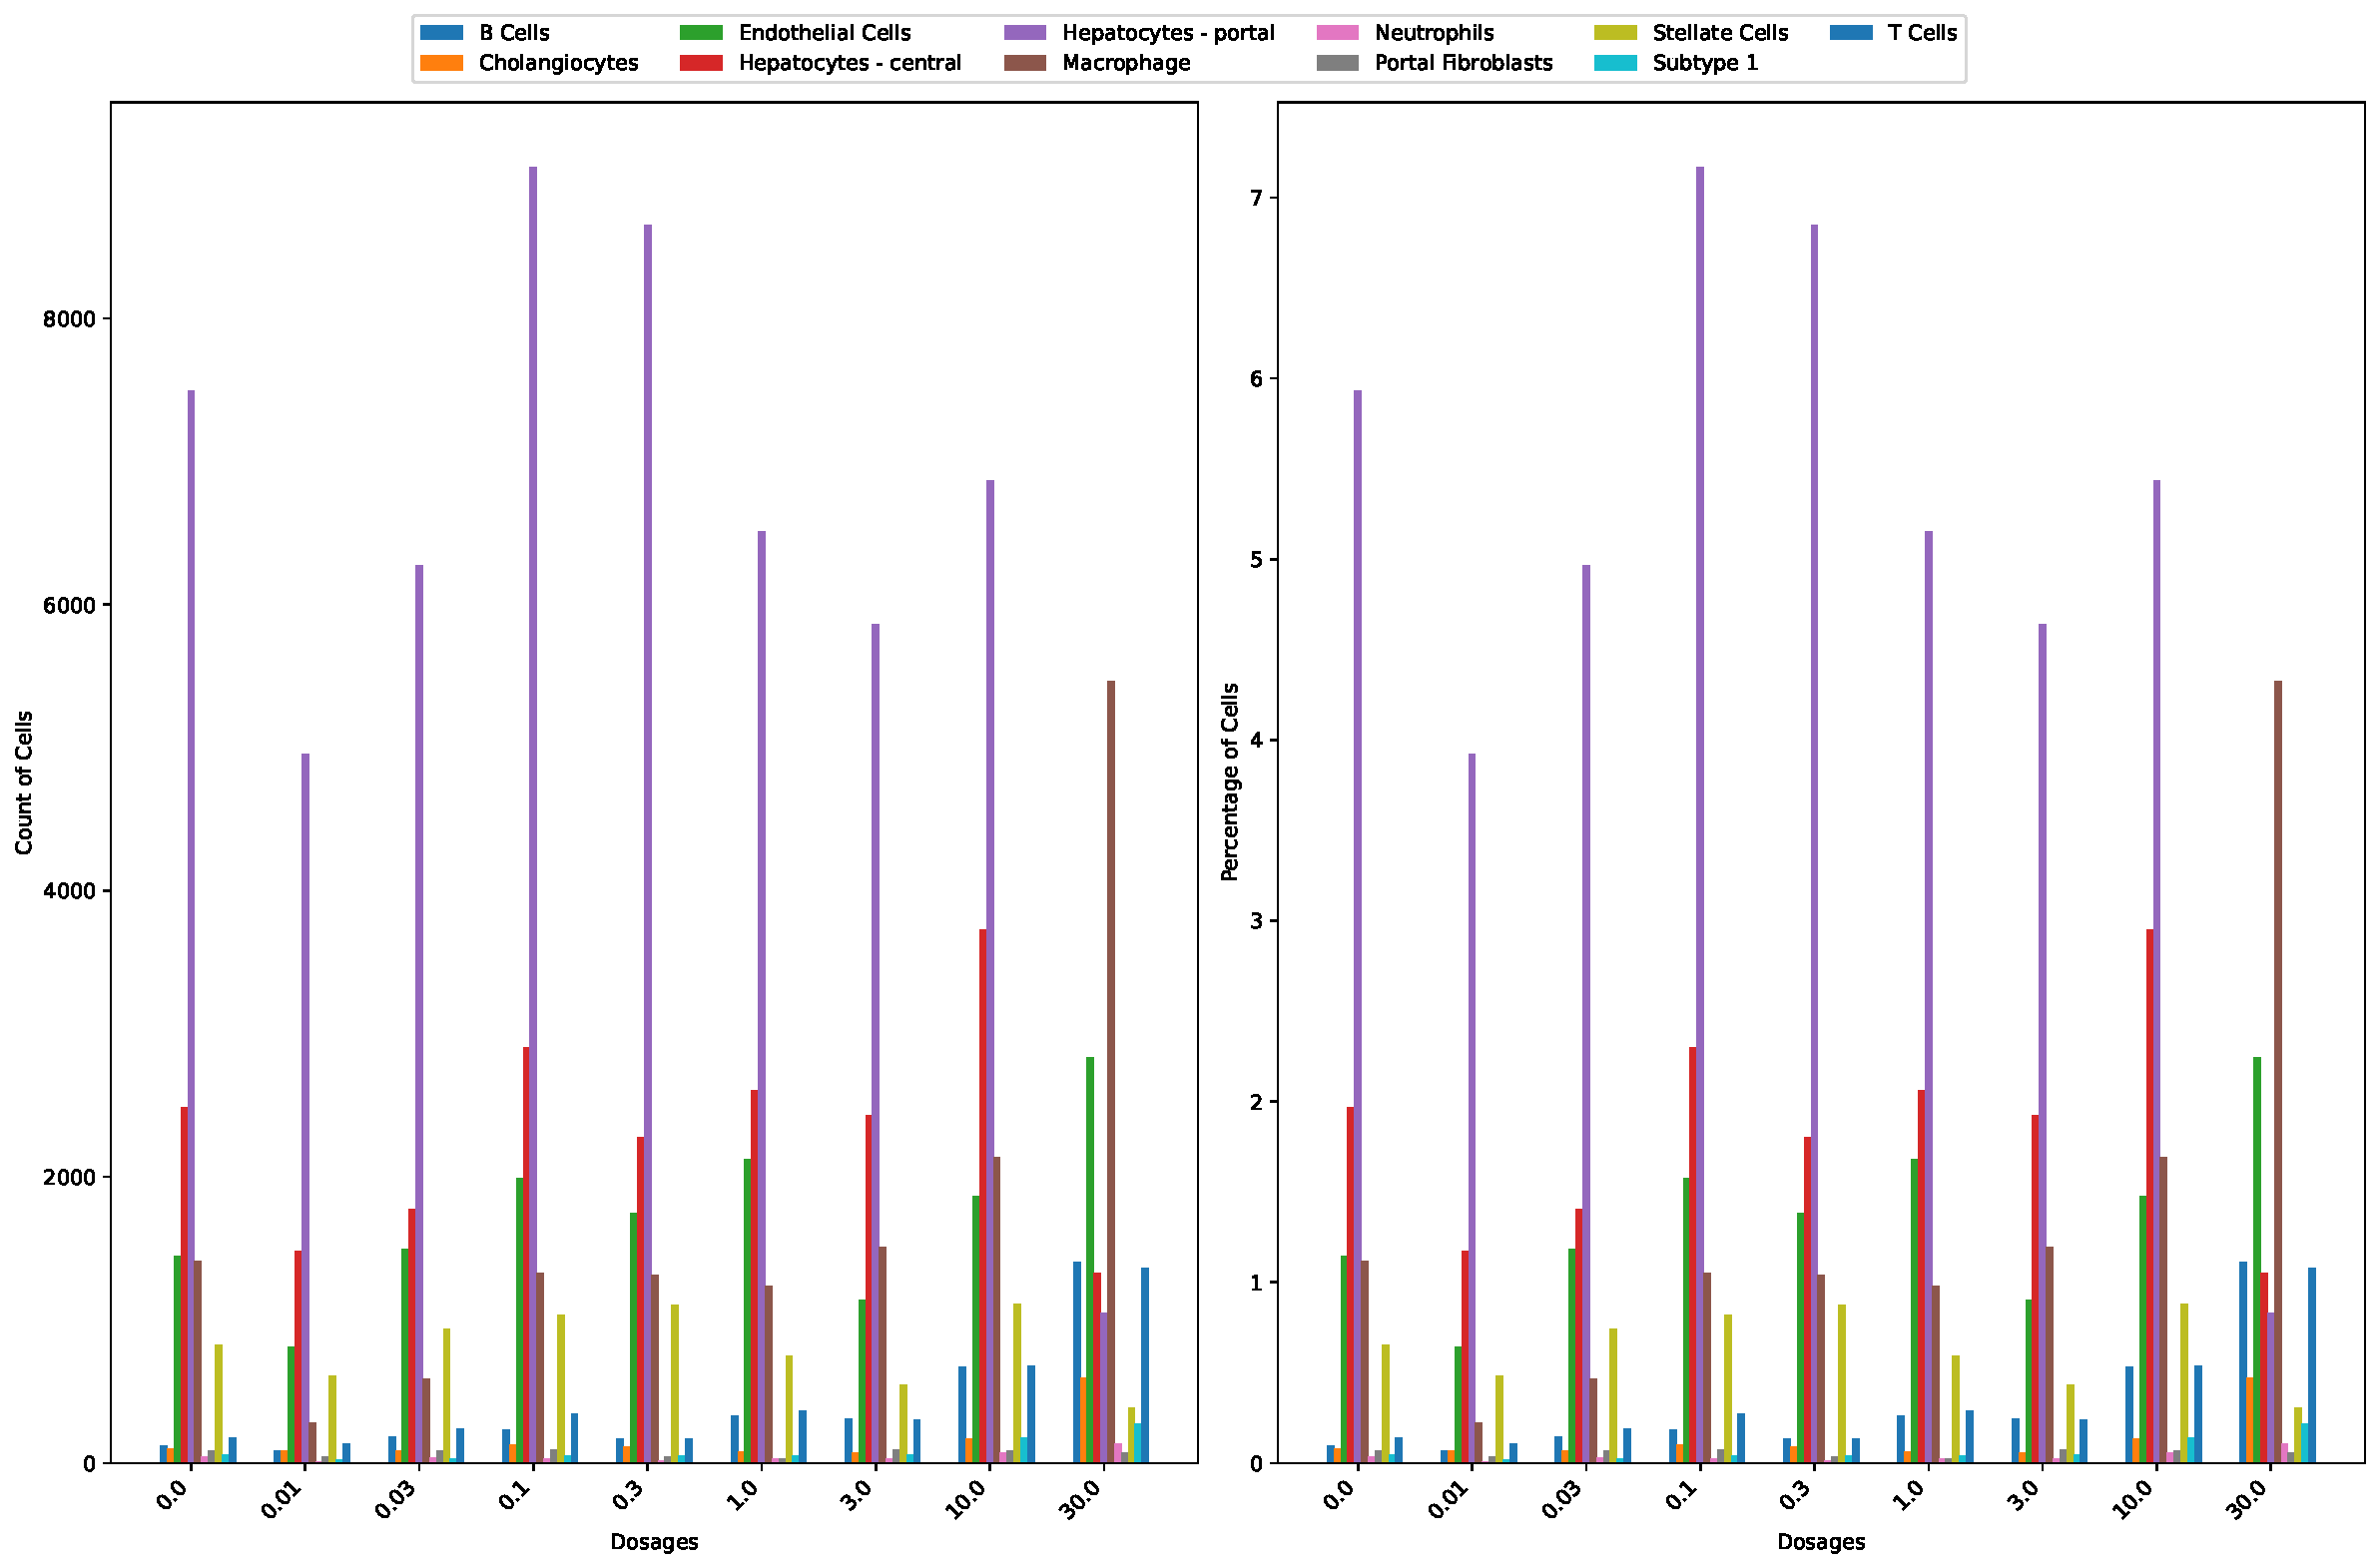
\includegraphics[width=.7\textwidth]{figures/nault_cell_types_counts.pdf}
        \caption{}
        \label{fig:figure4}
    \end{subfigure}    
    \caption{Nault overview}
    \label{fig:combined}
\end{figure}



\begin{figure}
    \centering
    \begin{minipage}{0.4\textwidth}
        \centering
        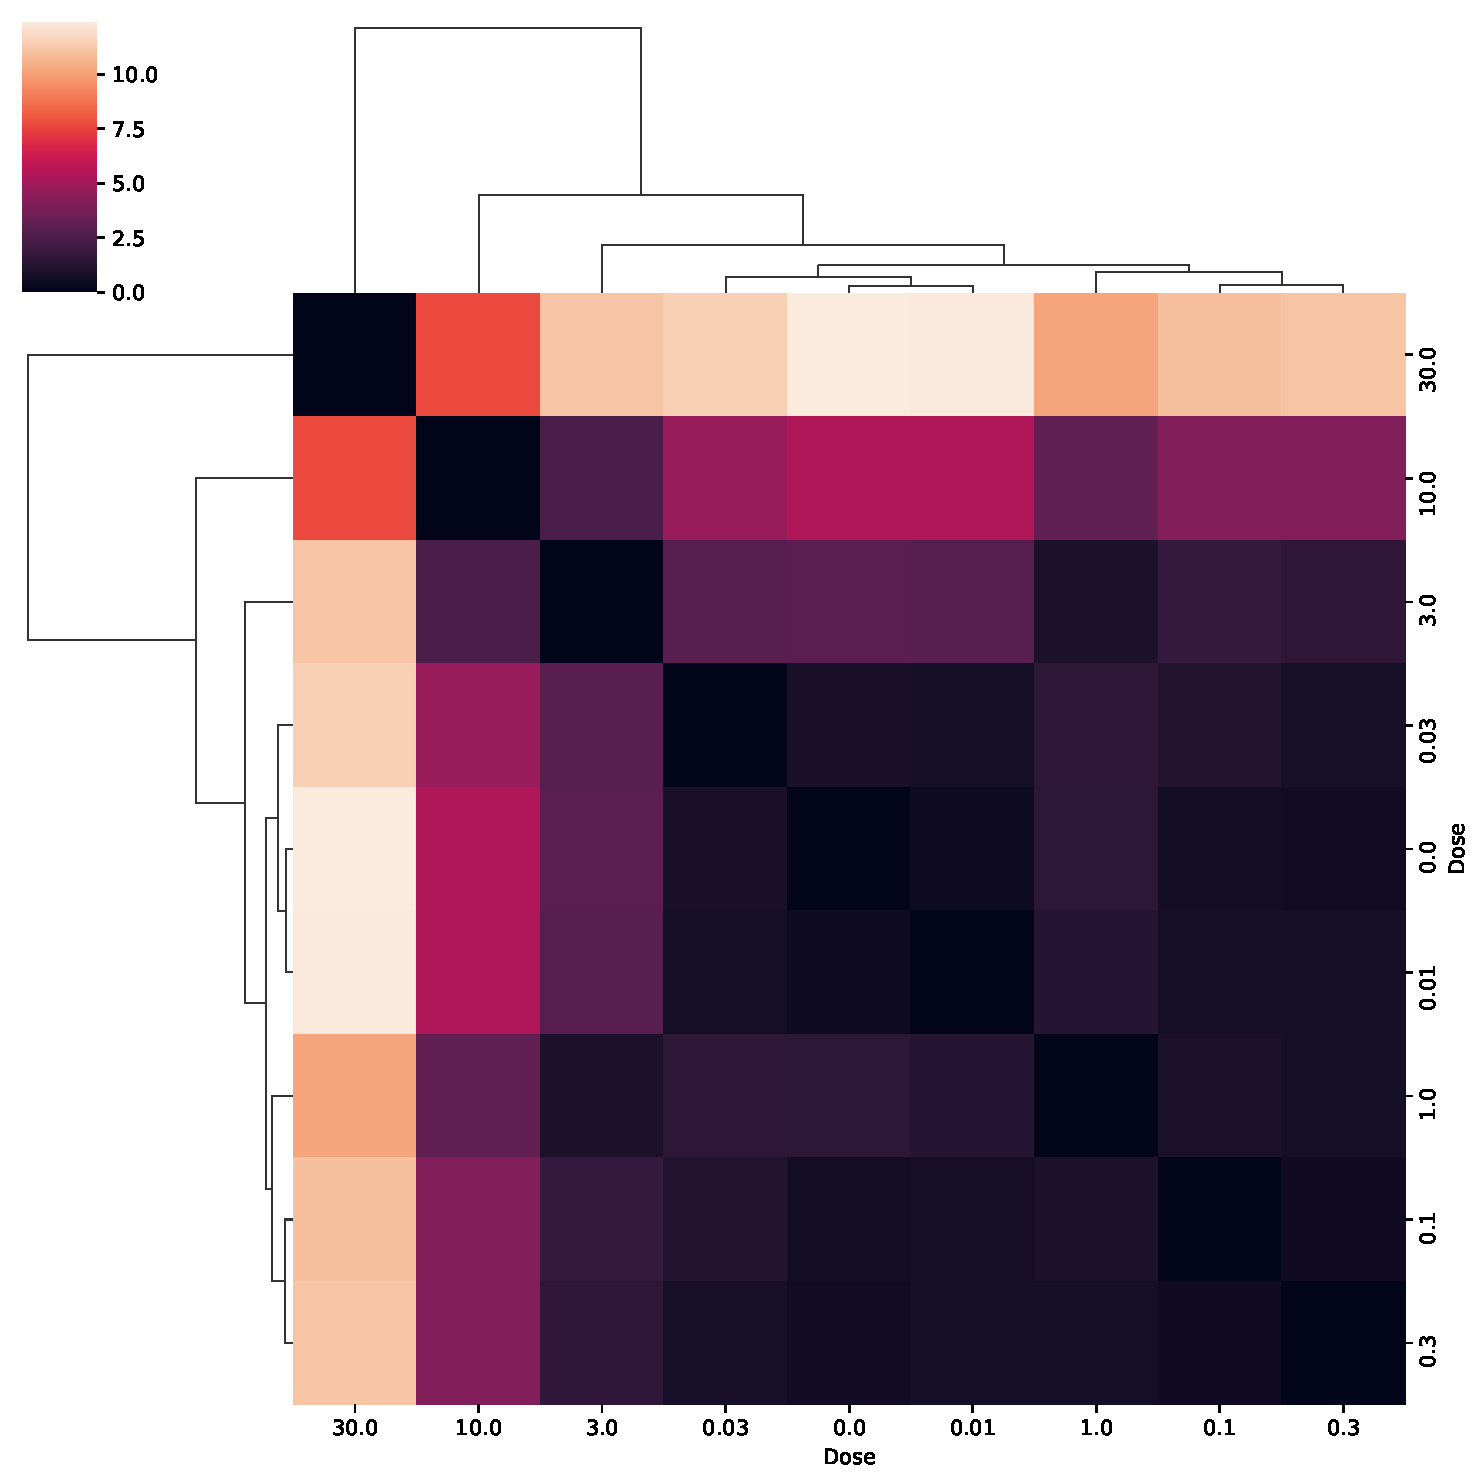
\includegraphics[width=\textwidth]{figures/nault_edistance_clustermap.pdf}
        \caption{E-distance}
    \end{minipage} \hfill
    \begin{minipage}{0.4\textwidth}
        \centering
        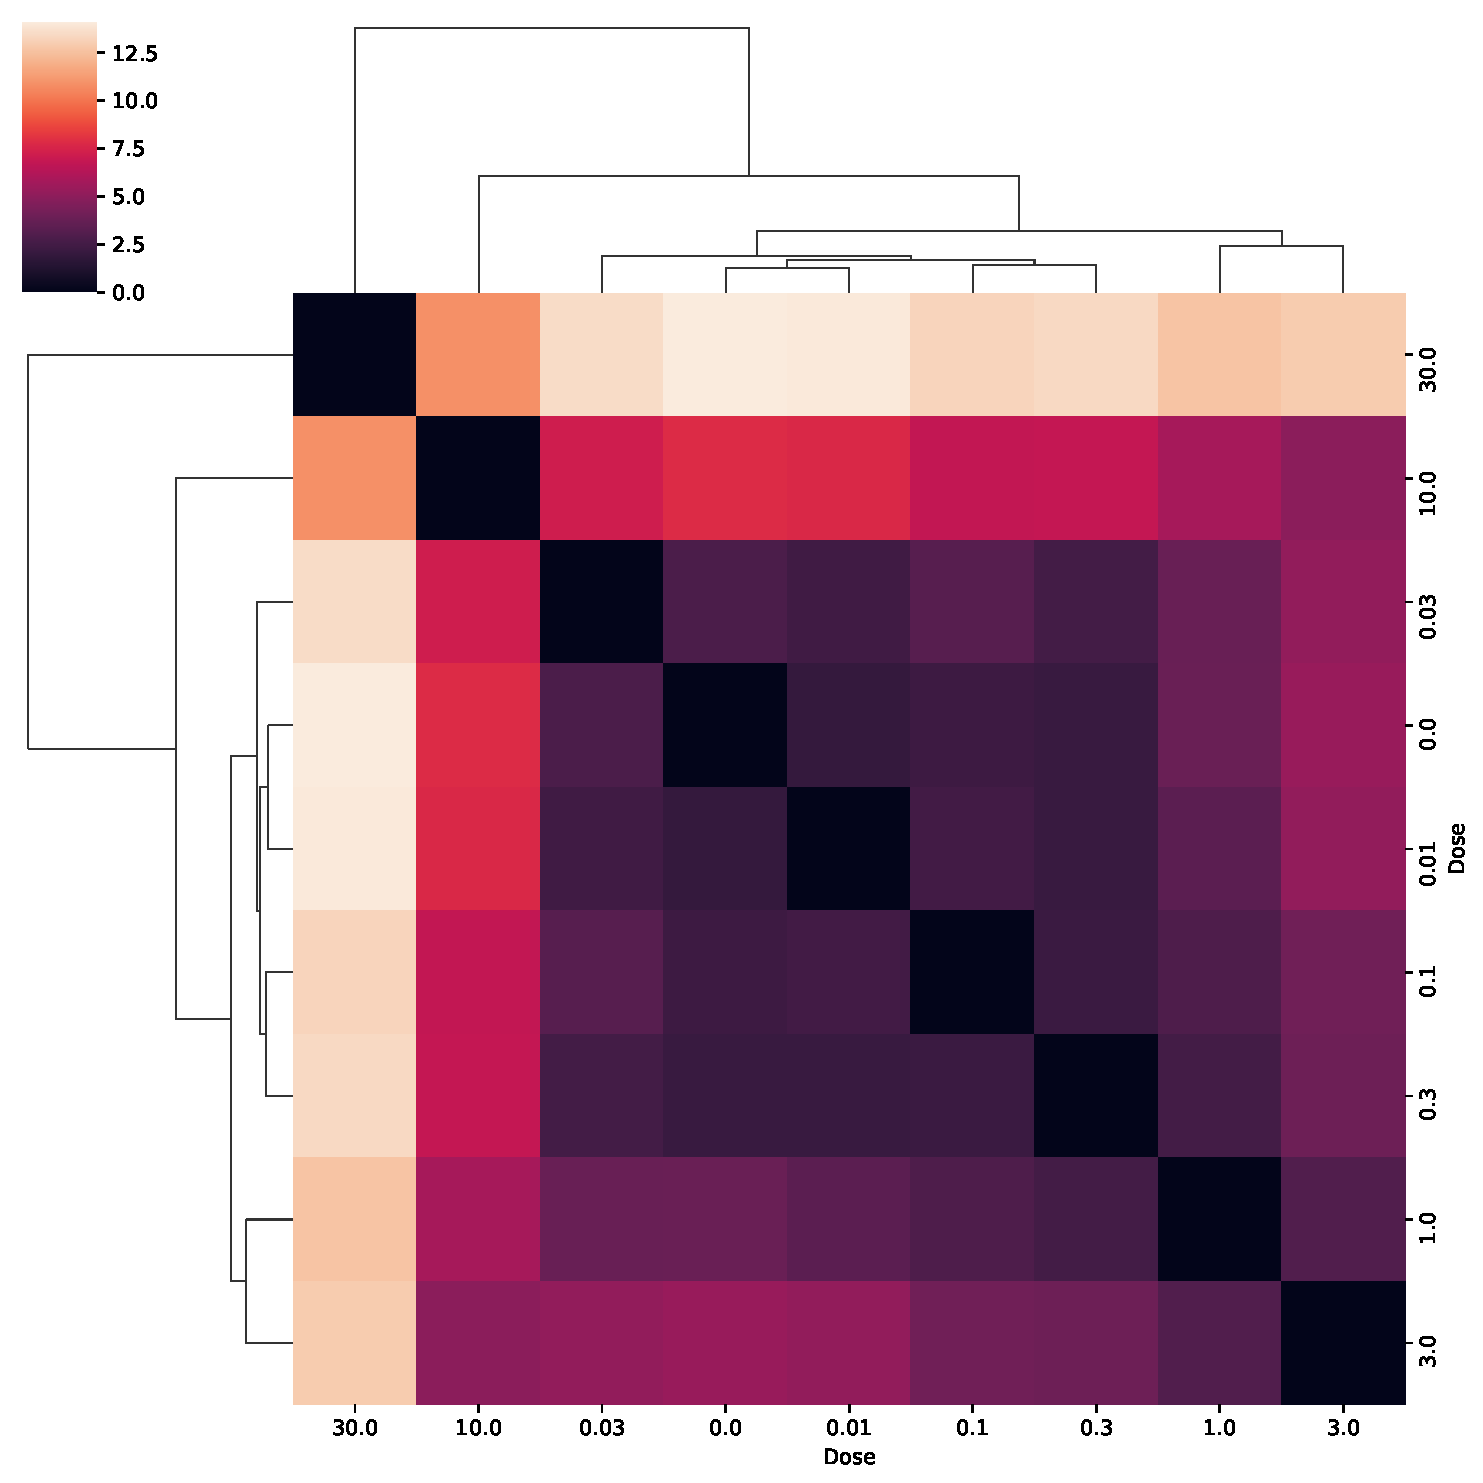
\includegraphics[width=\textwidth]{figures/nault_euclidean_clustermap.pdf}
        \caption{Euclidean}
    \end{minipage}
    \vskip\baselineskip

    \begin{minipage}{0.4\textwidth}
        \centering
        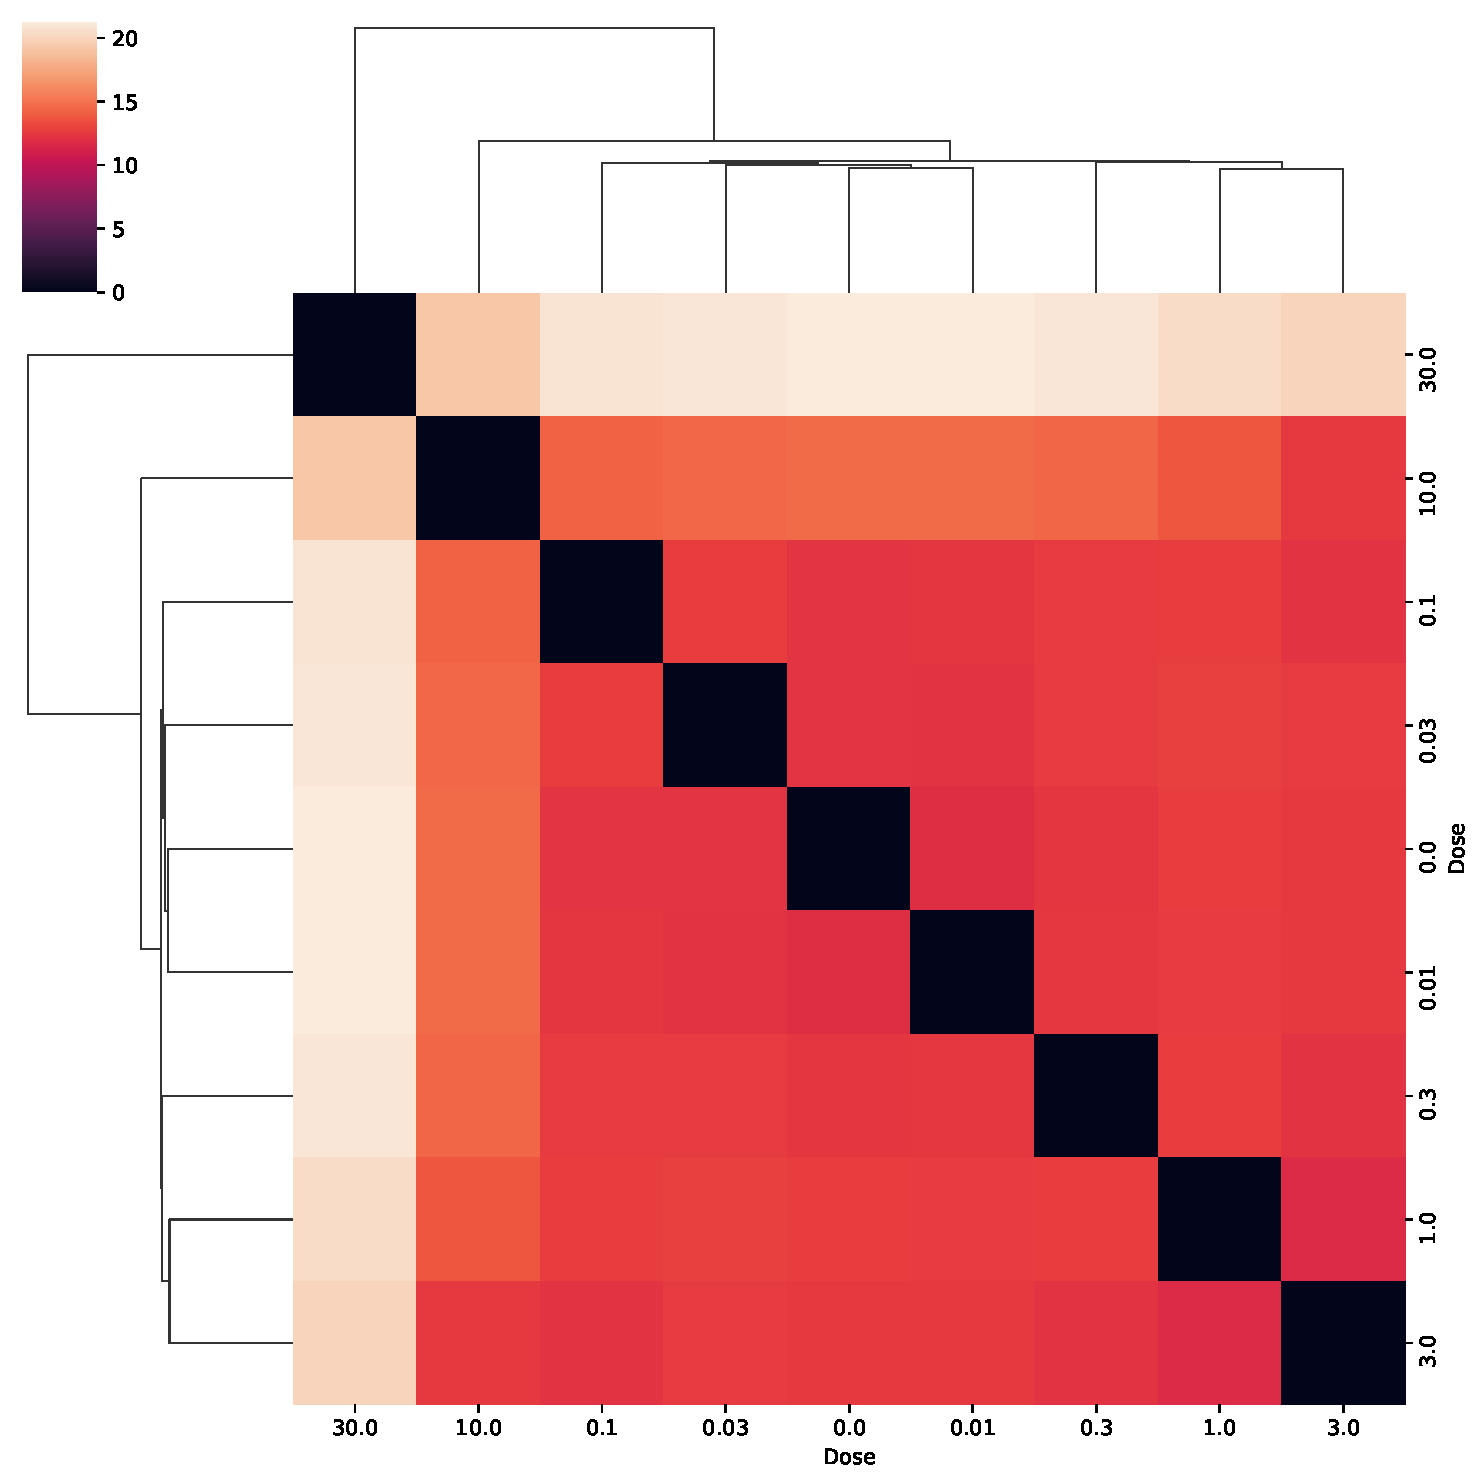
\includegraphics[width=\textwidth]{figures/nault_mean_pairwise_clustermap.pdf}
        \caption{Mean pairwise}
    \end{minipage} \hfill
    \begin{minipage}{0.4\textwidth}
        \centering
        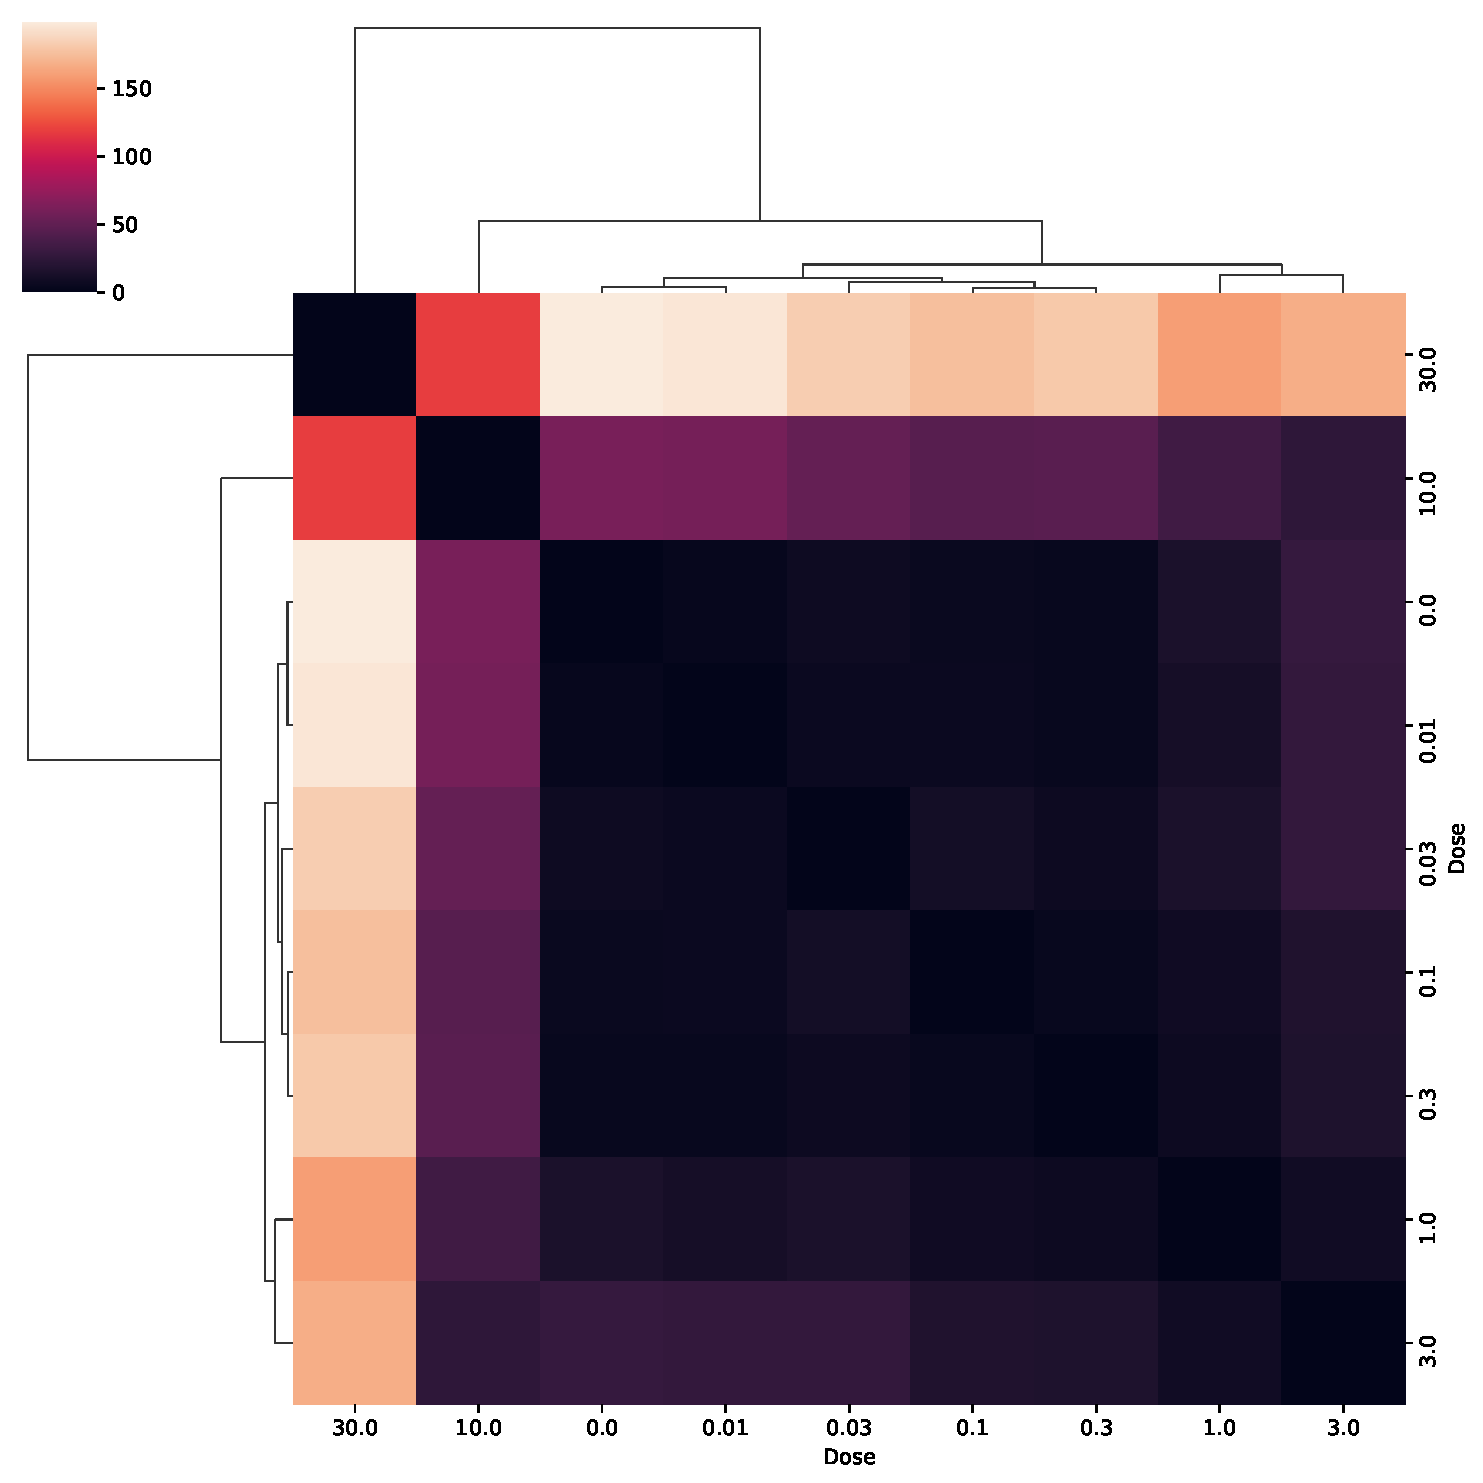
\includegraphics[width=\textwidth]{figures/nault_mmd_clustermap.pdf}
        \caption{MMD}
    \end{minipage}
    \vskip\baselineskip

    \begin{minipage}{0.4\textwidth}
        \centering
        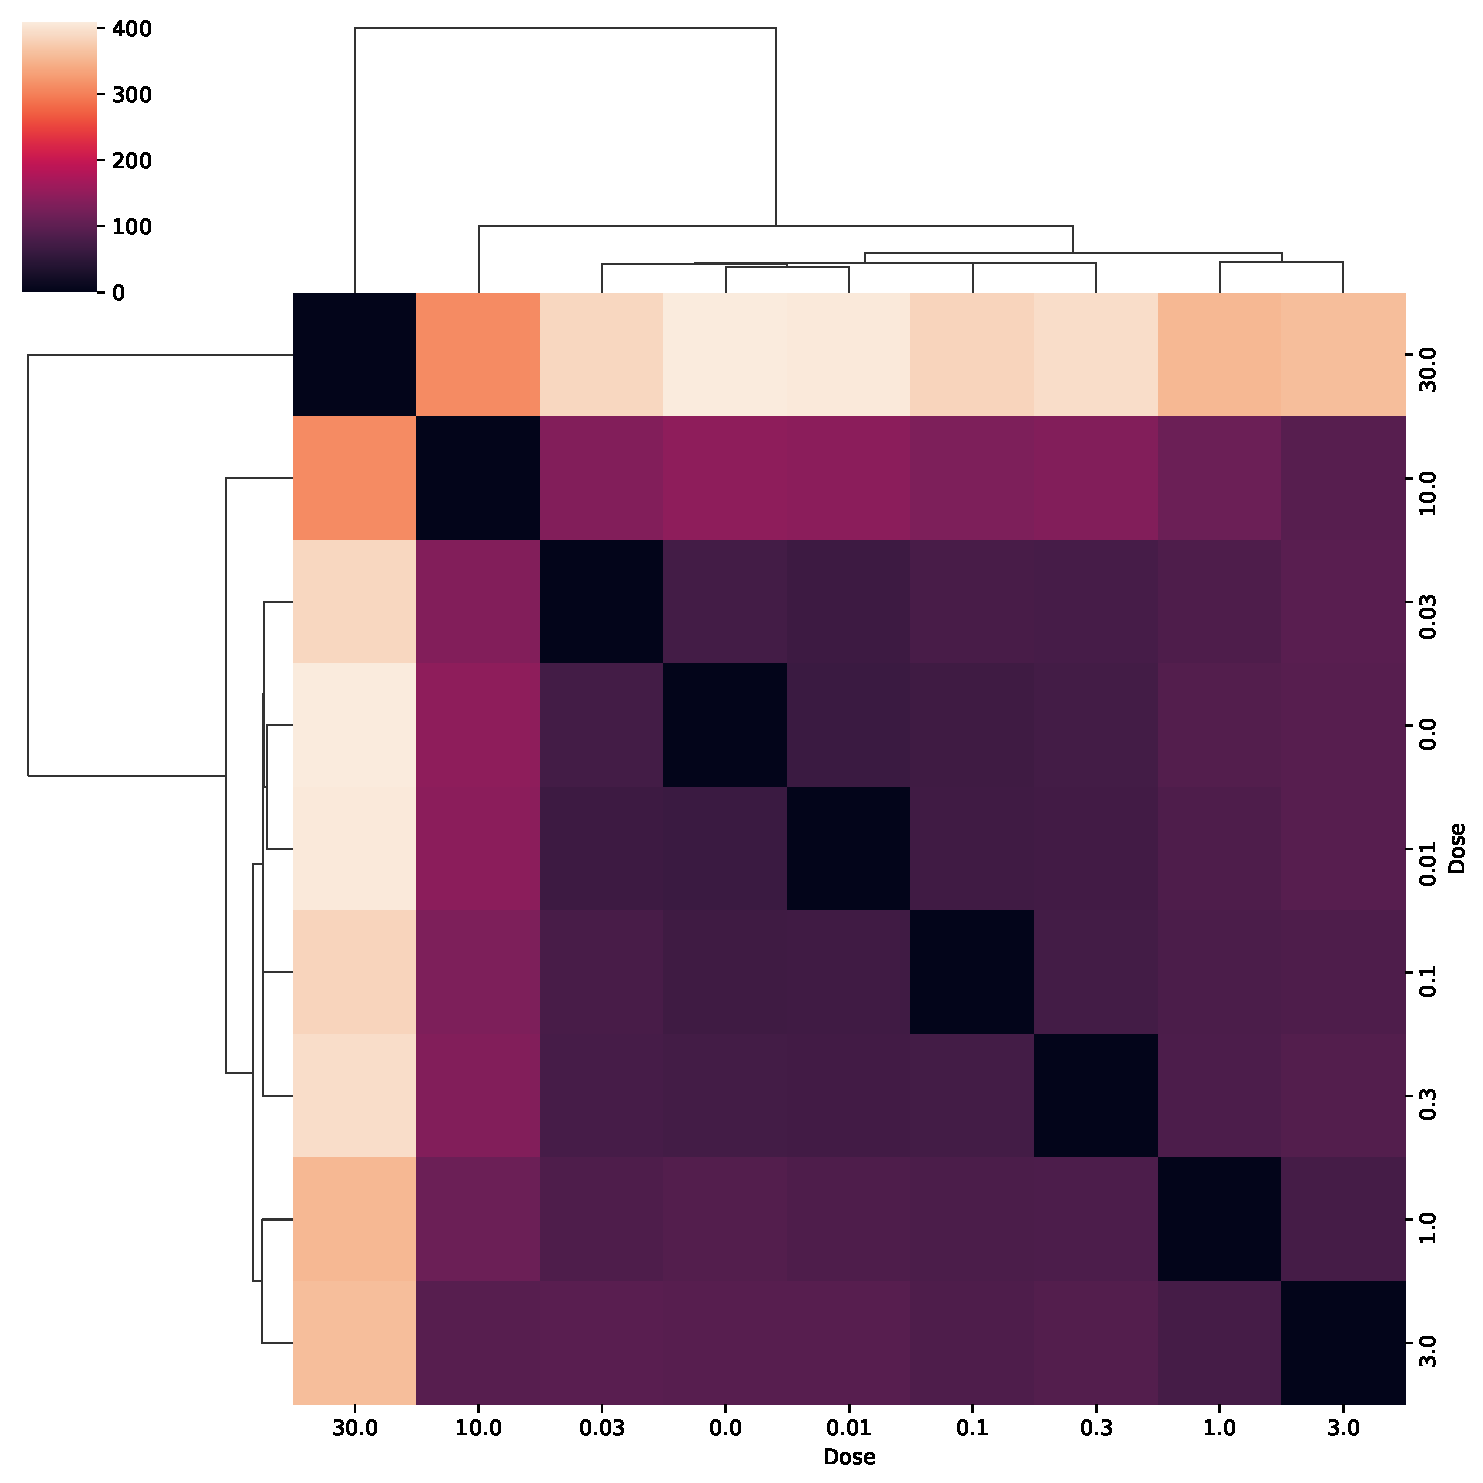
\includegraphics[width=\textwidth]{figures/nault_wasserstein_clustermap.pdf}
        \caption{Wasserstein}
    \end{minipage}
    \caption{Distance metrics across all cell types per dosage}
\end{figure}

\begin{figure}
    \centering
    \begin{minipage}{0.4\textwidth}
        \centering
        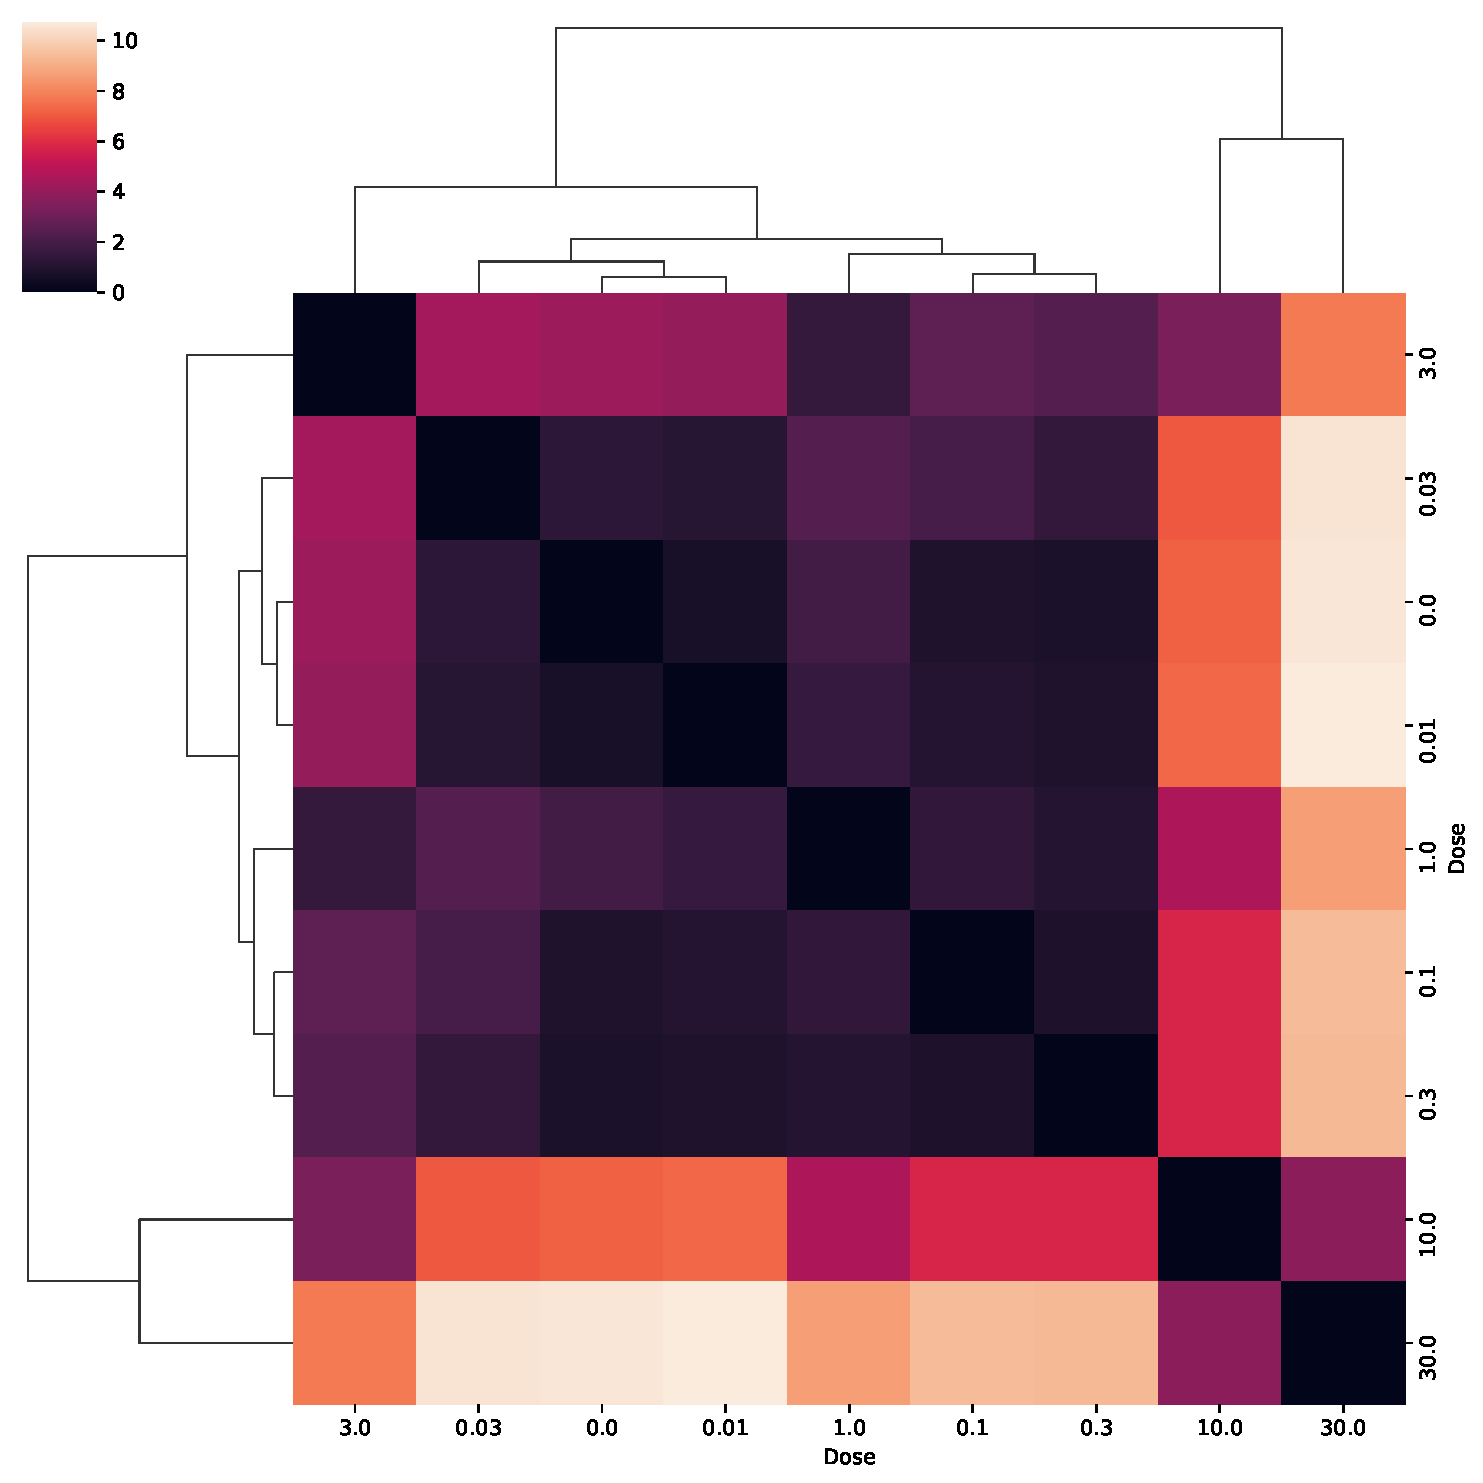
\includegraphics[width=\textwidth]{figures/hepatocytes_edistance_clustermap.pdf}
        \caption{E-distance}
    \end{minipage} \hfill
    \begin{minipage}{0.4\textwidth}
        \centering
        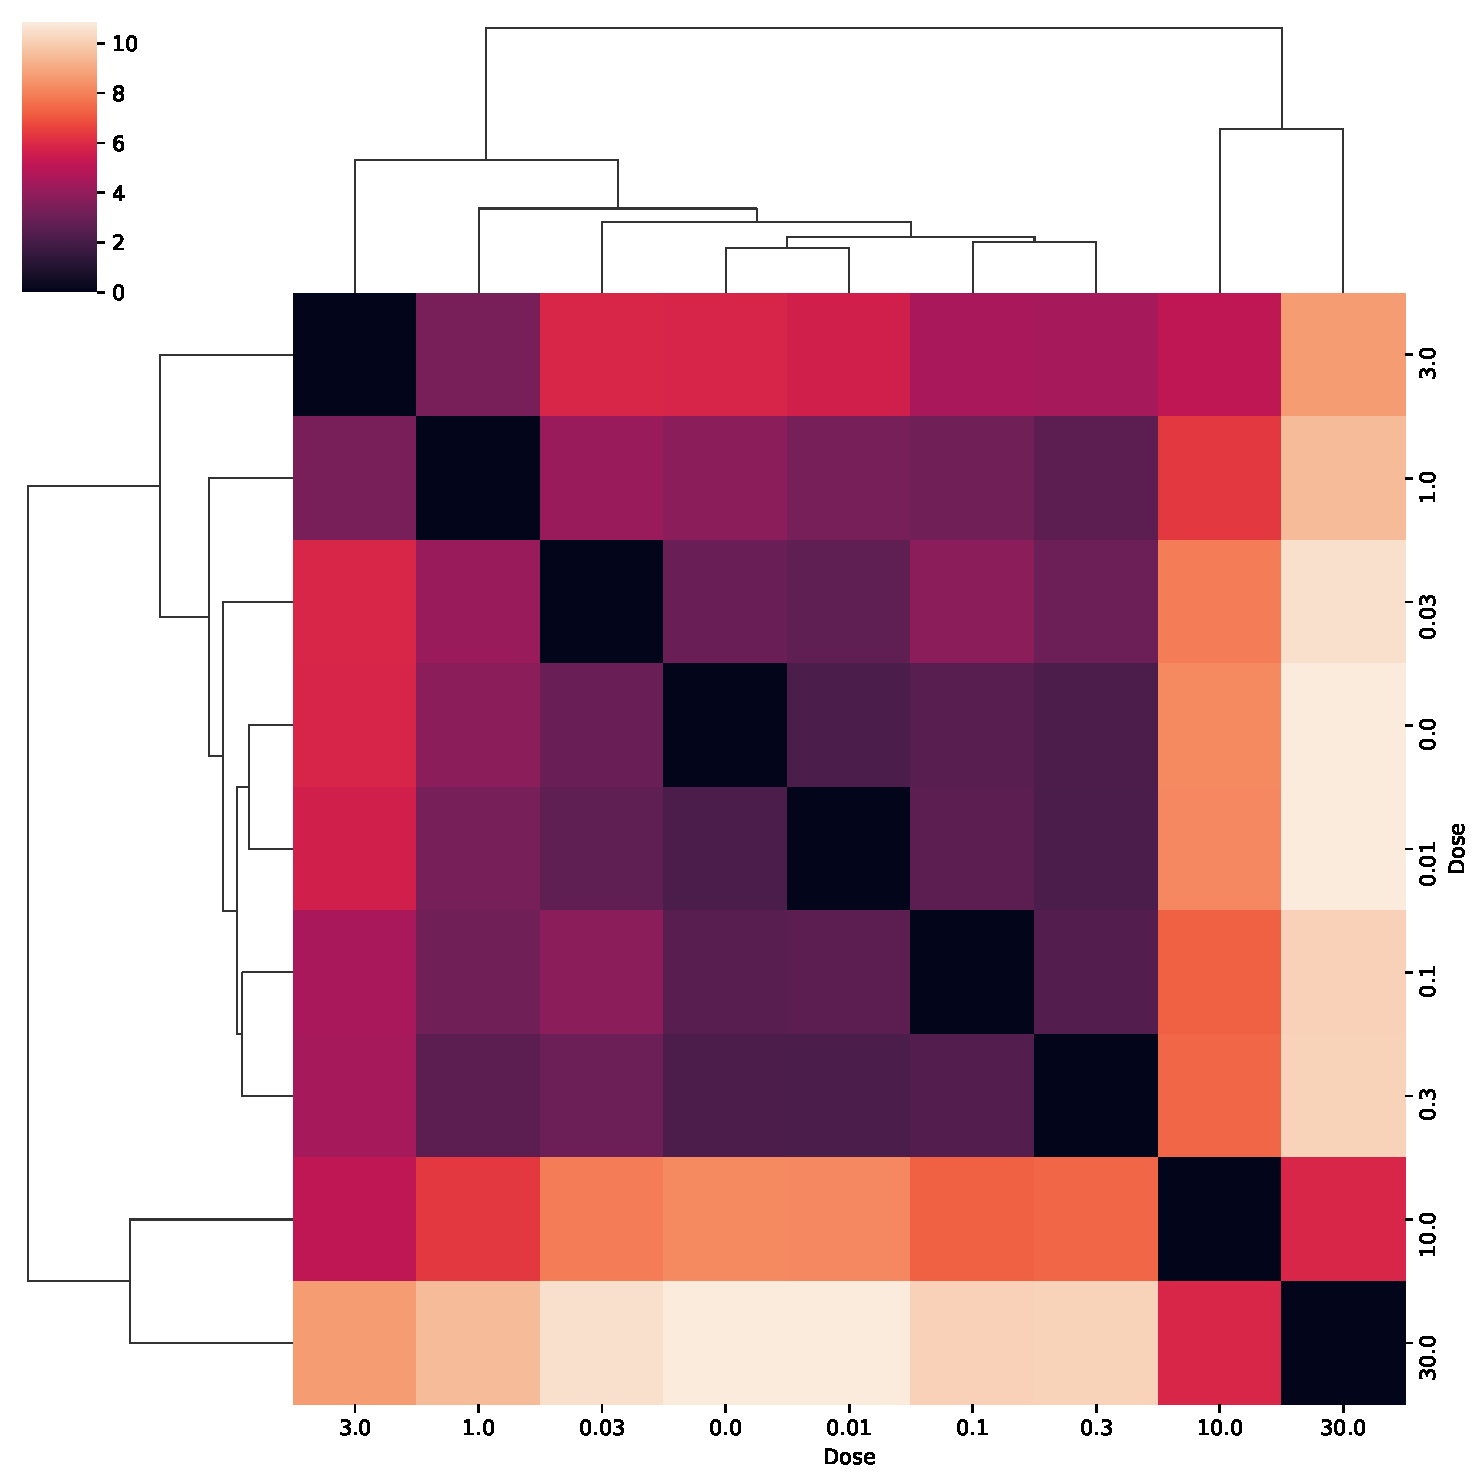
\includegraphics[width=\textwidth]{figures/hepatocytes_euclidean_clustermap.pdf}
        \caption{Euclidean}
    \end{minipage}
    \vskip\baselineskip

    \begin{minipage}{0.4\textwidth}
        \centering
        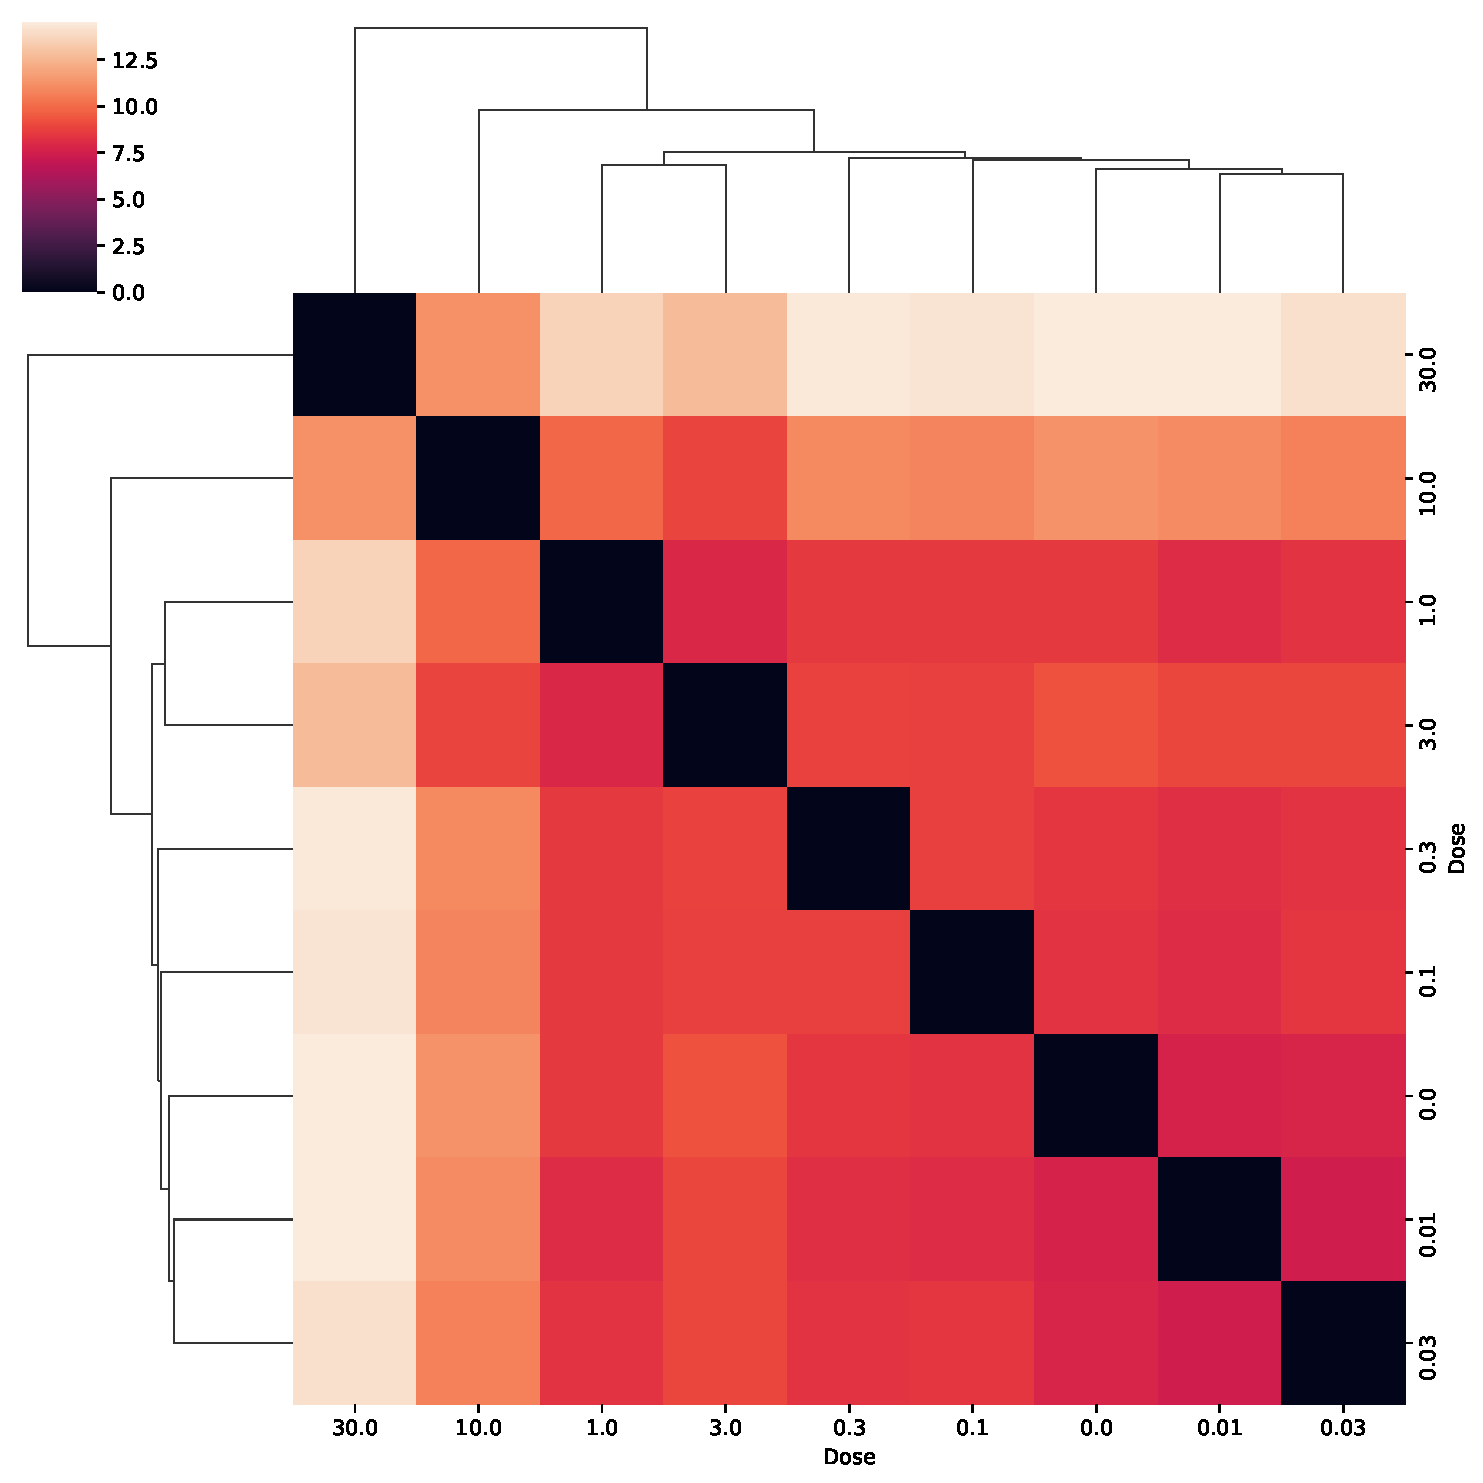
\includegraphics[width=\textwidth]{figures/hepatocytes_mean_pairwise_clustermap.pdf}
        \caption{Mean pairwise}
    \end{minipage} \hfill
    \begin{minipage}{0.4\textwidth}
        \centering
        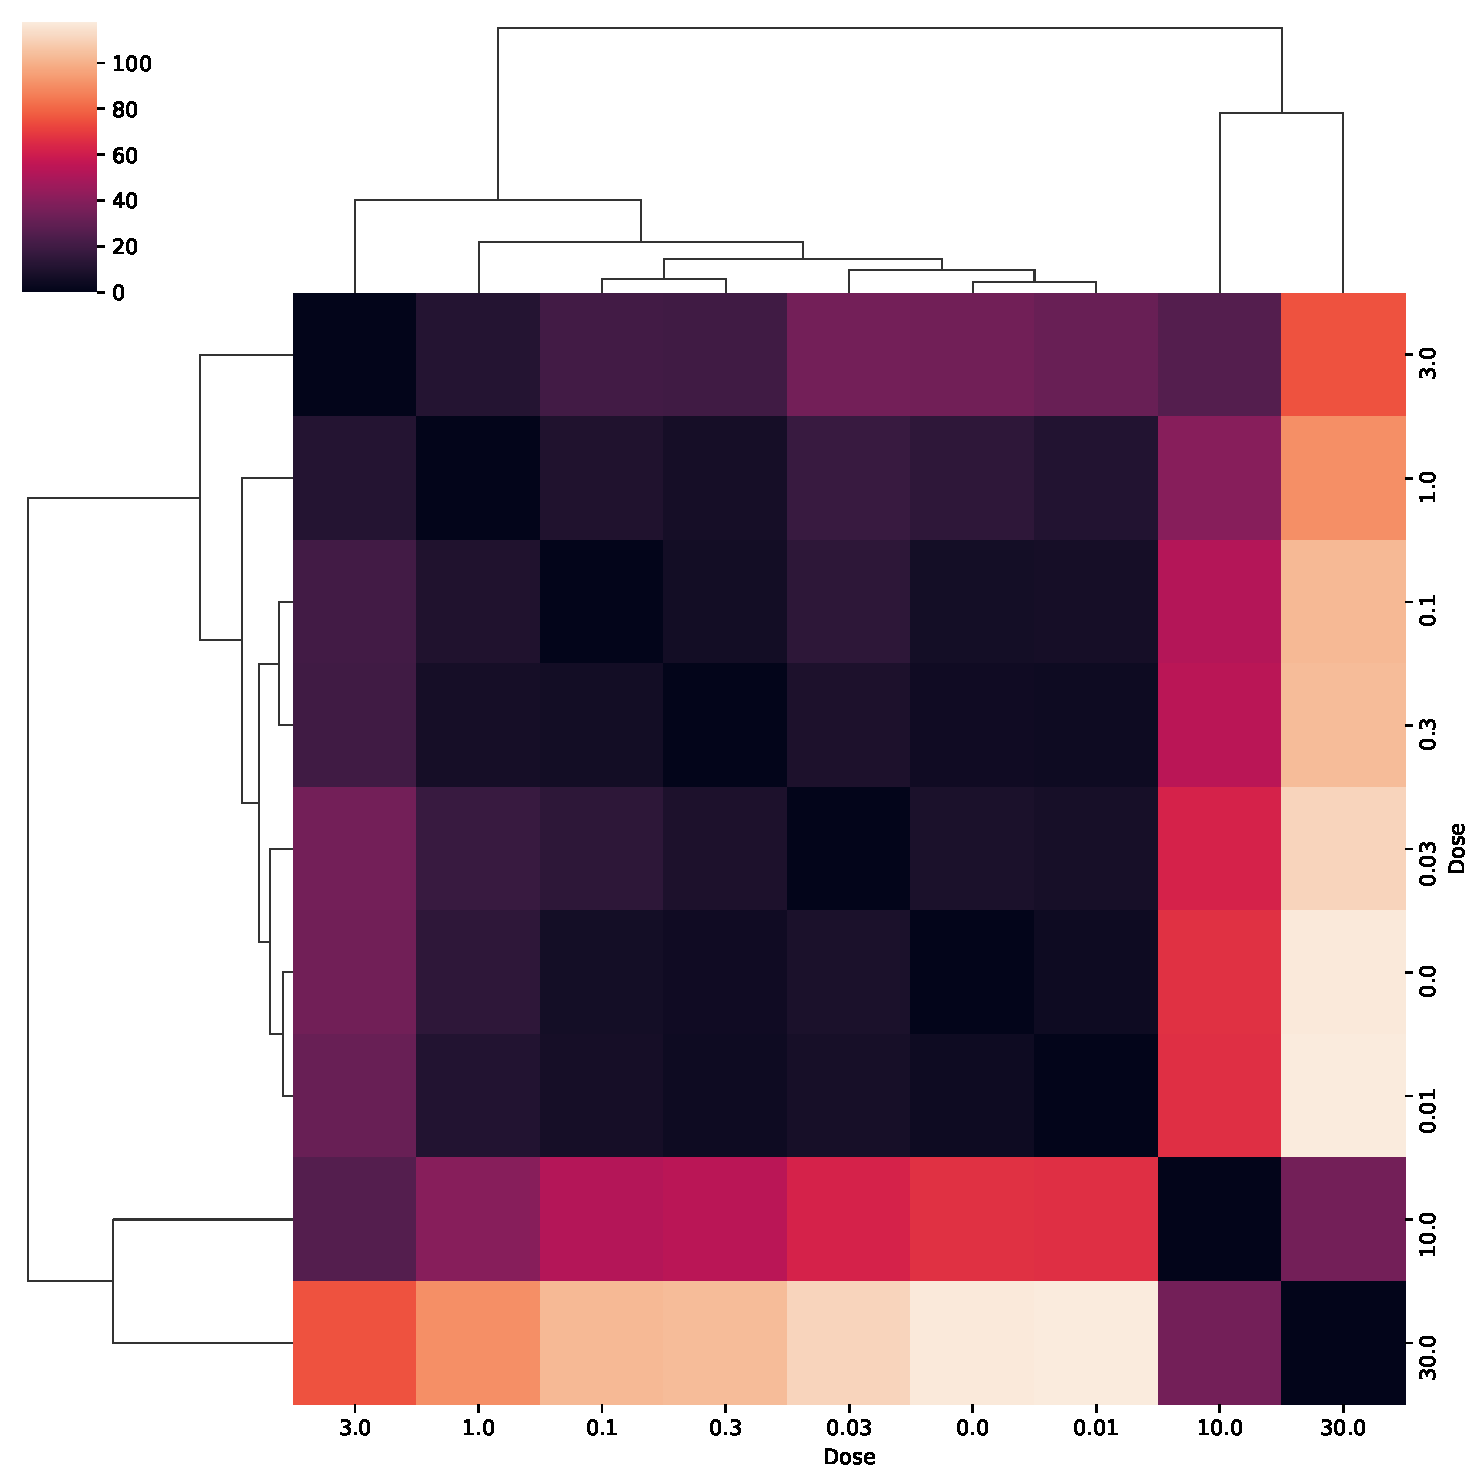
\includegraphics[width=\textwidth]{figures/hepatocytes_mmd_clustermap.pdf}
        \caption{MMD}
    \end{minipage}
    \vskip\baselineskip

    \begin{minipage}{0.4\textwidth}
        \centering
        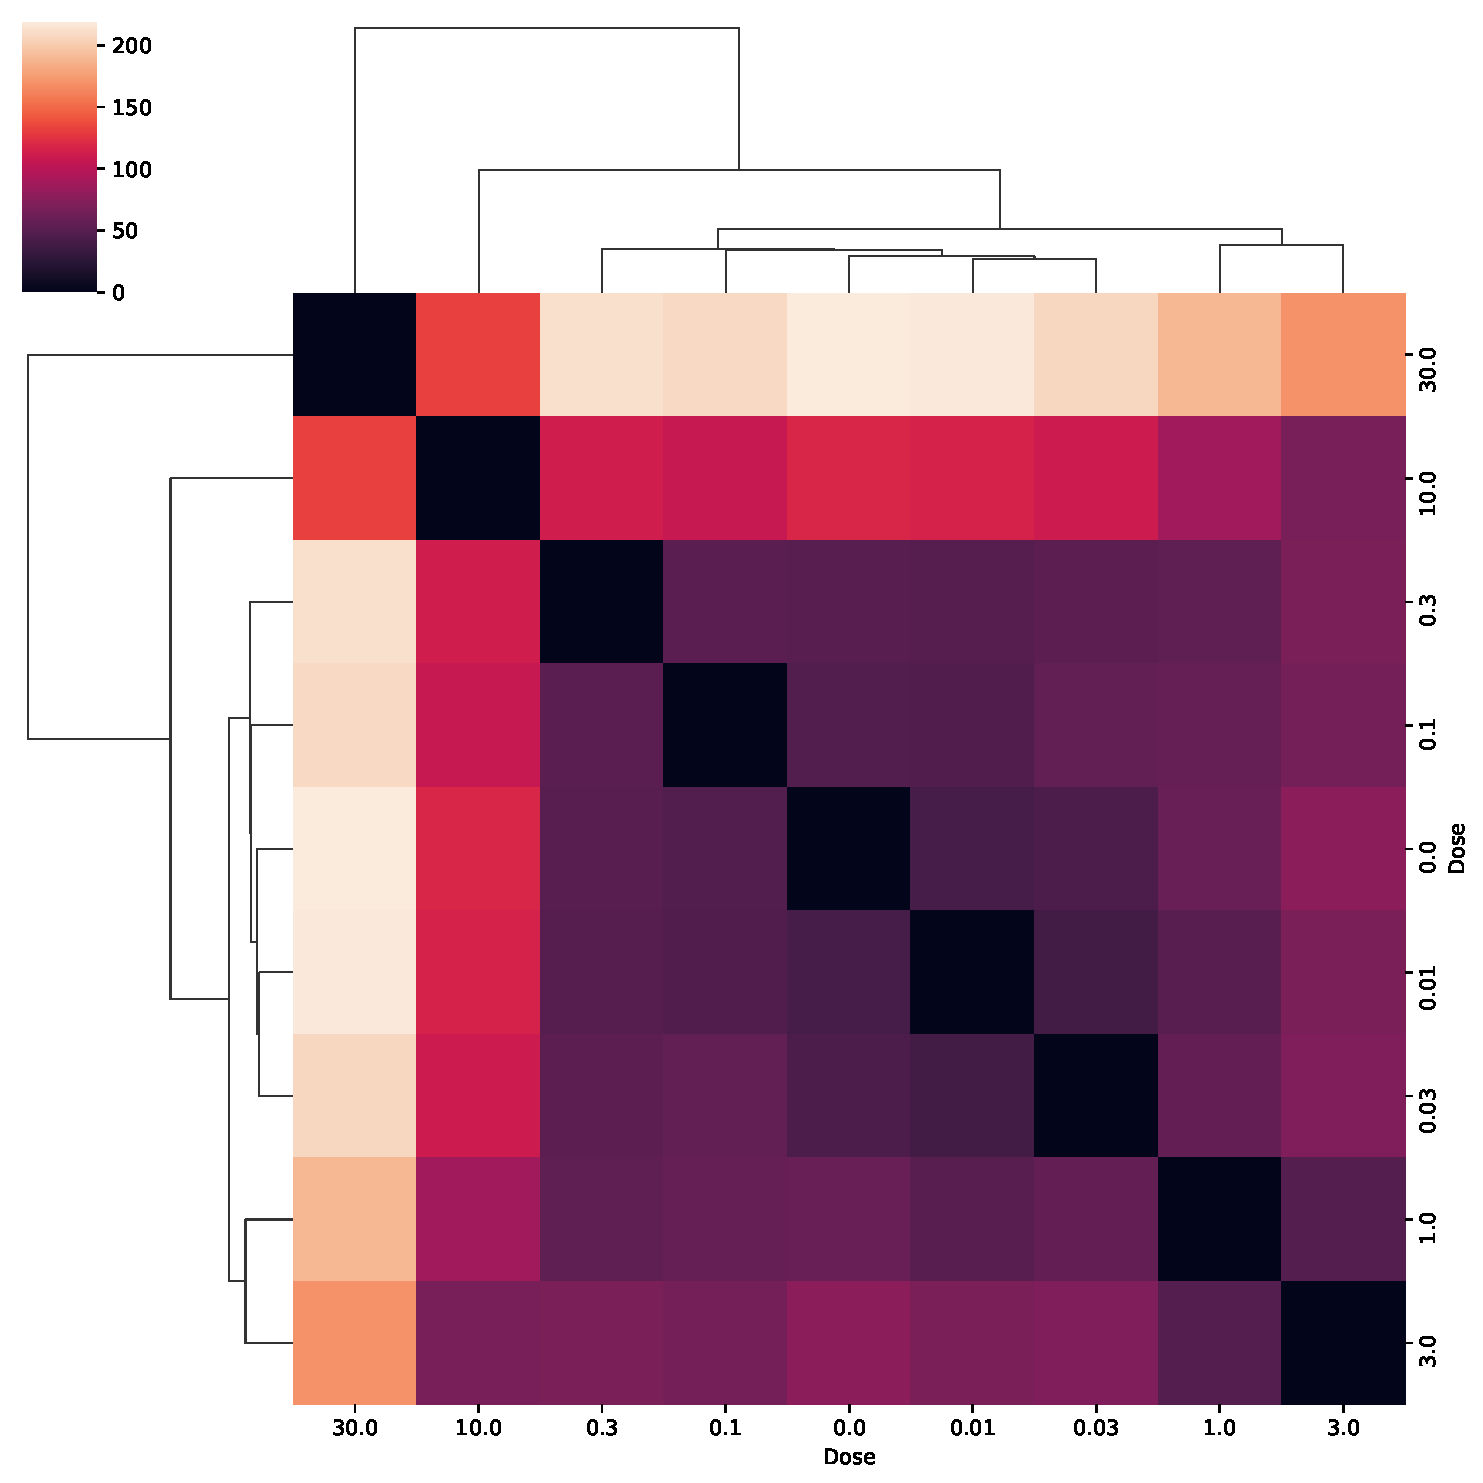
\includegraphics[width=\textwidth]{figures/hepatocytes_wasserstein_clustermap.pdf}
        \caption{Wasserstein}
    \end{minipage}
    \caption{Distance metrics for cell type Hepatocytes - portal per dosage}
\end{figure}

\begin{figure}
    \centering
    \begin{minipage}{0.4\textwidth}
        \centering
        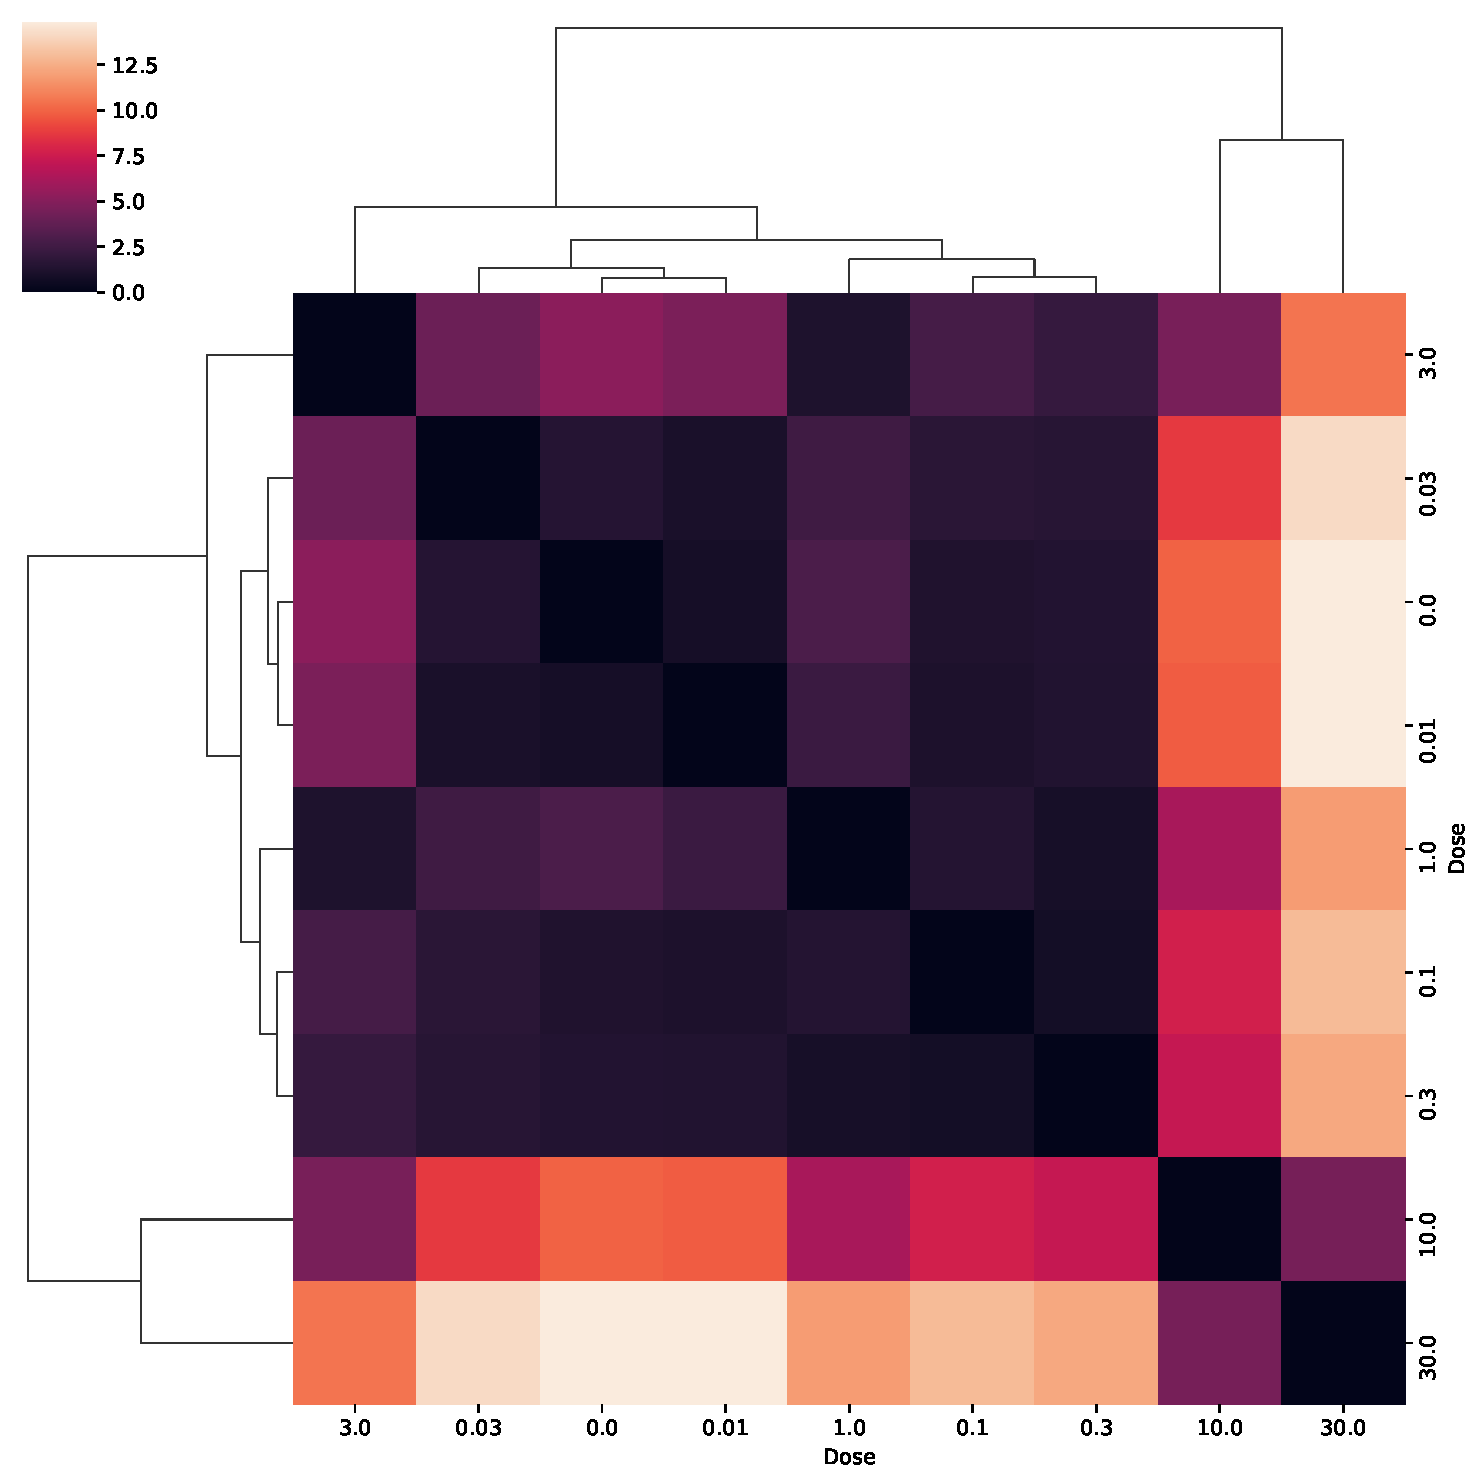
\includegraphics[width=\textwidth]{figures/hepatocytes_central_edistance_clustermap.pdf}
        \caption{E-distance}
    \end{minipage} \hfill
    \begin{minipage}{0.4\textwidth}
        \centering
        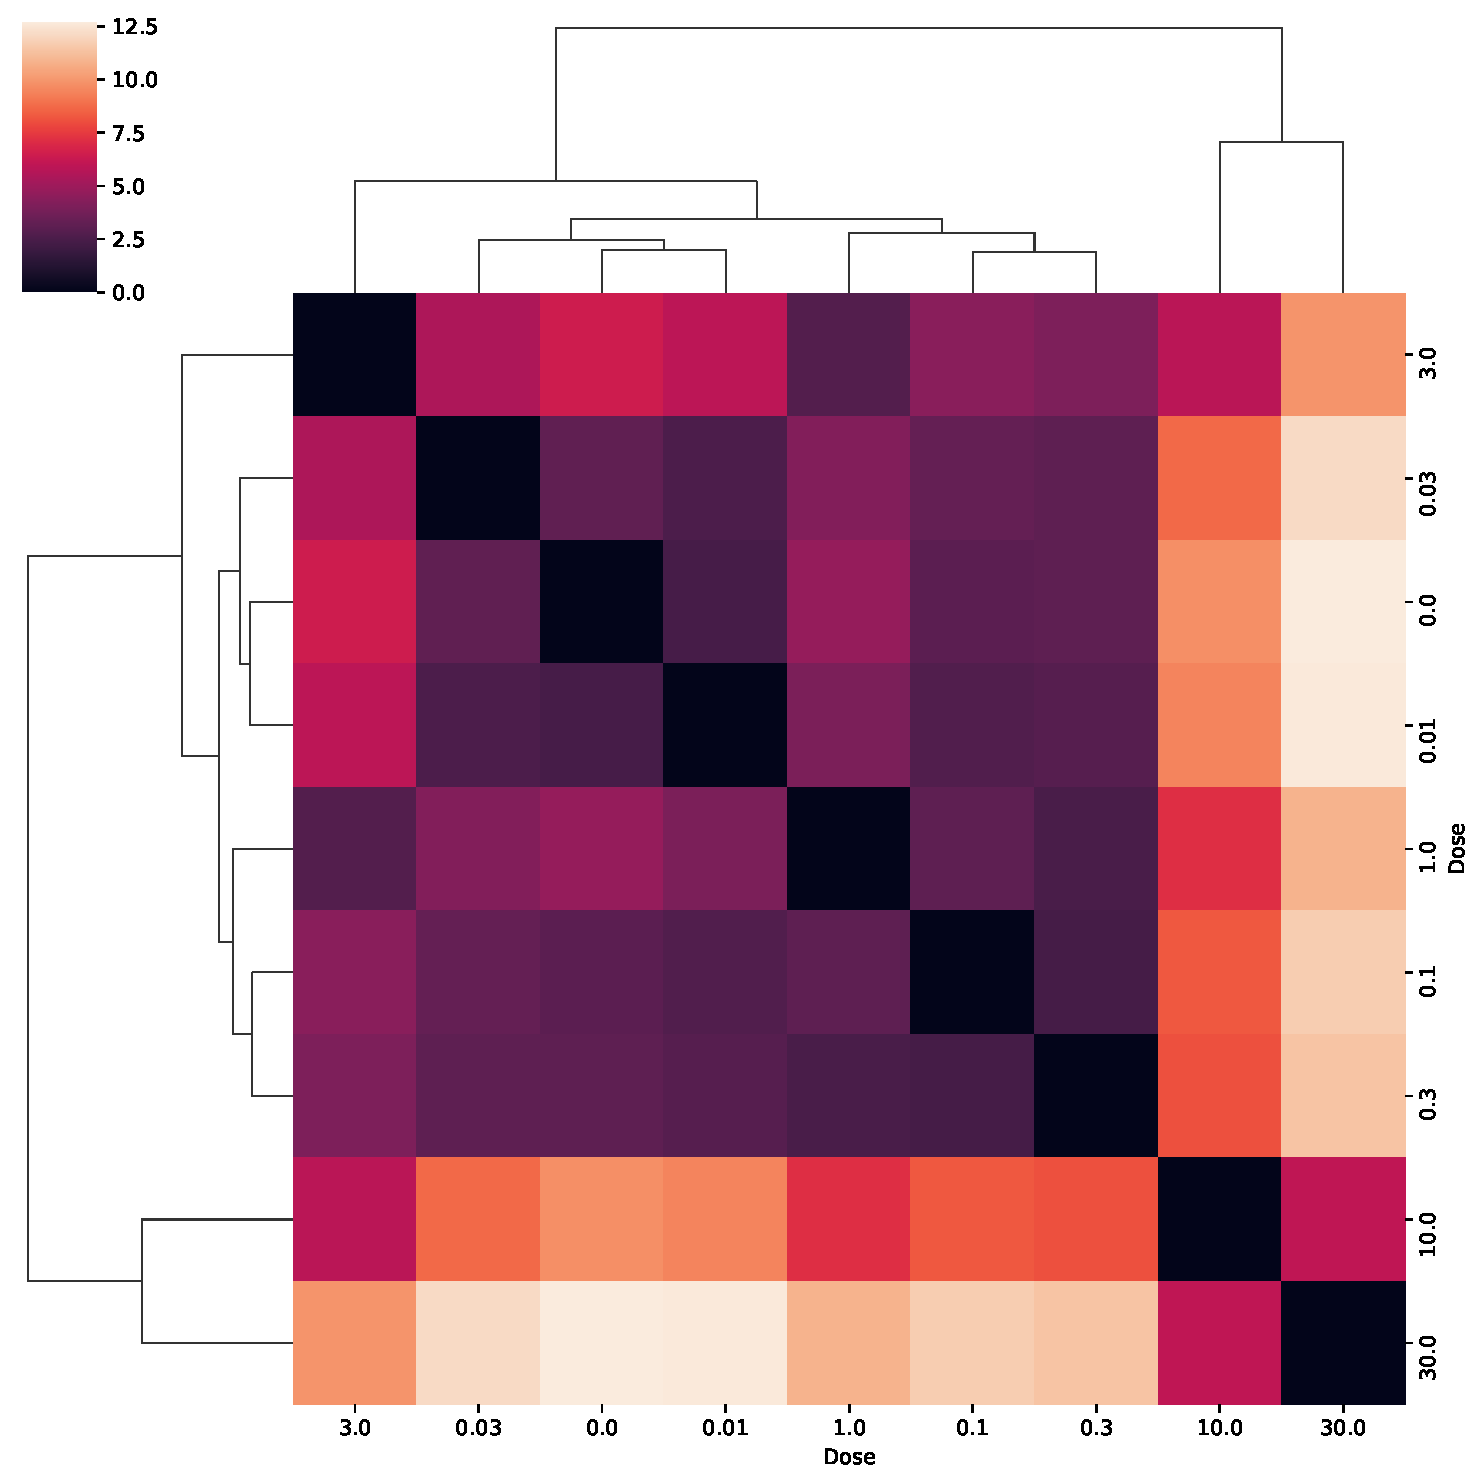
\includegraphics[width=\textwidth]{figures/hepatocytes_central_euclidean_clustermap.pdf}
        \caption{Euclidean}
    \end{minipage}
    \vskip\baselineskip

    \begin{minipage}{0.4\textwidth}
        \centering
        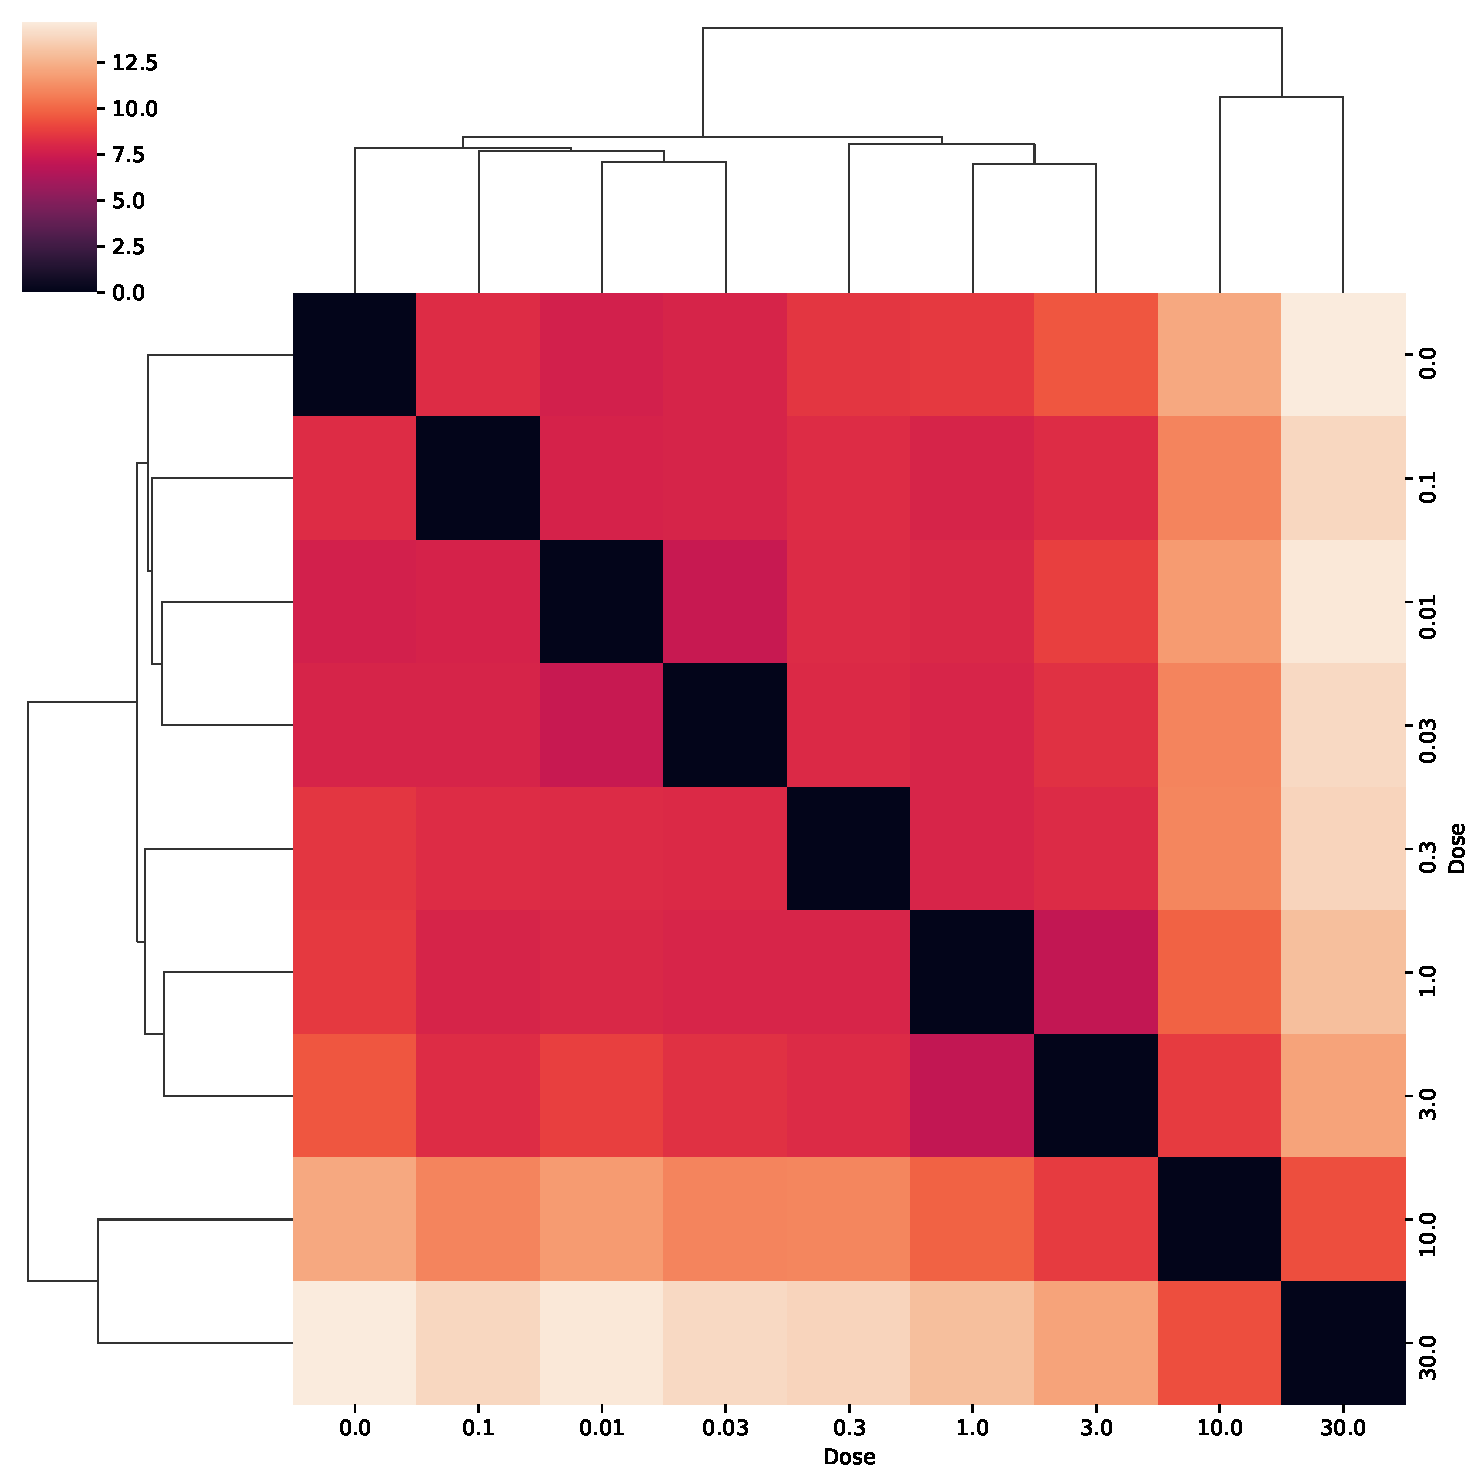
\includegraphics[width=\textwidth]{figures/hepatocytes_central_mean_pairwise_clustermap.pdf}
        \caption{Mean pairwise}
    \end{minipage} \hfill
    \begin{minipage}{0.4\textwidth}
        \centering
        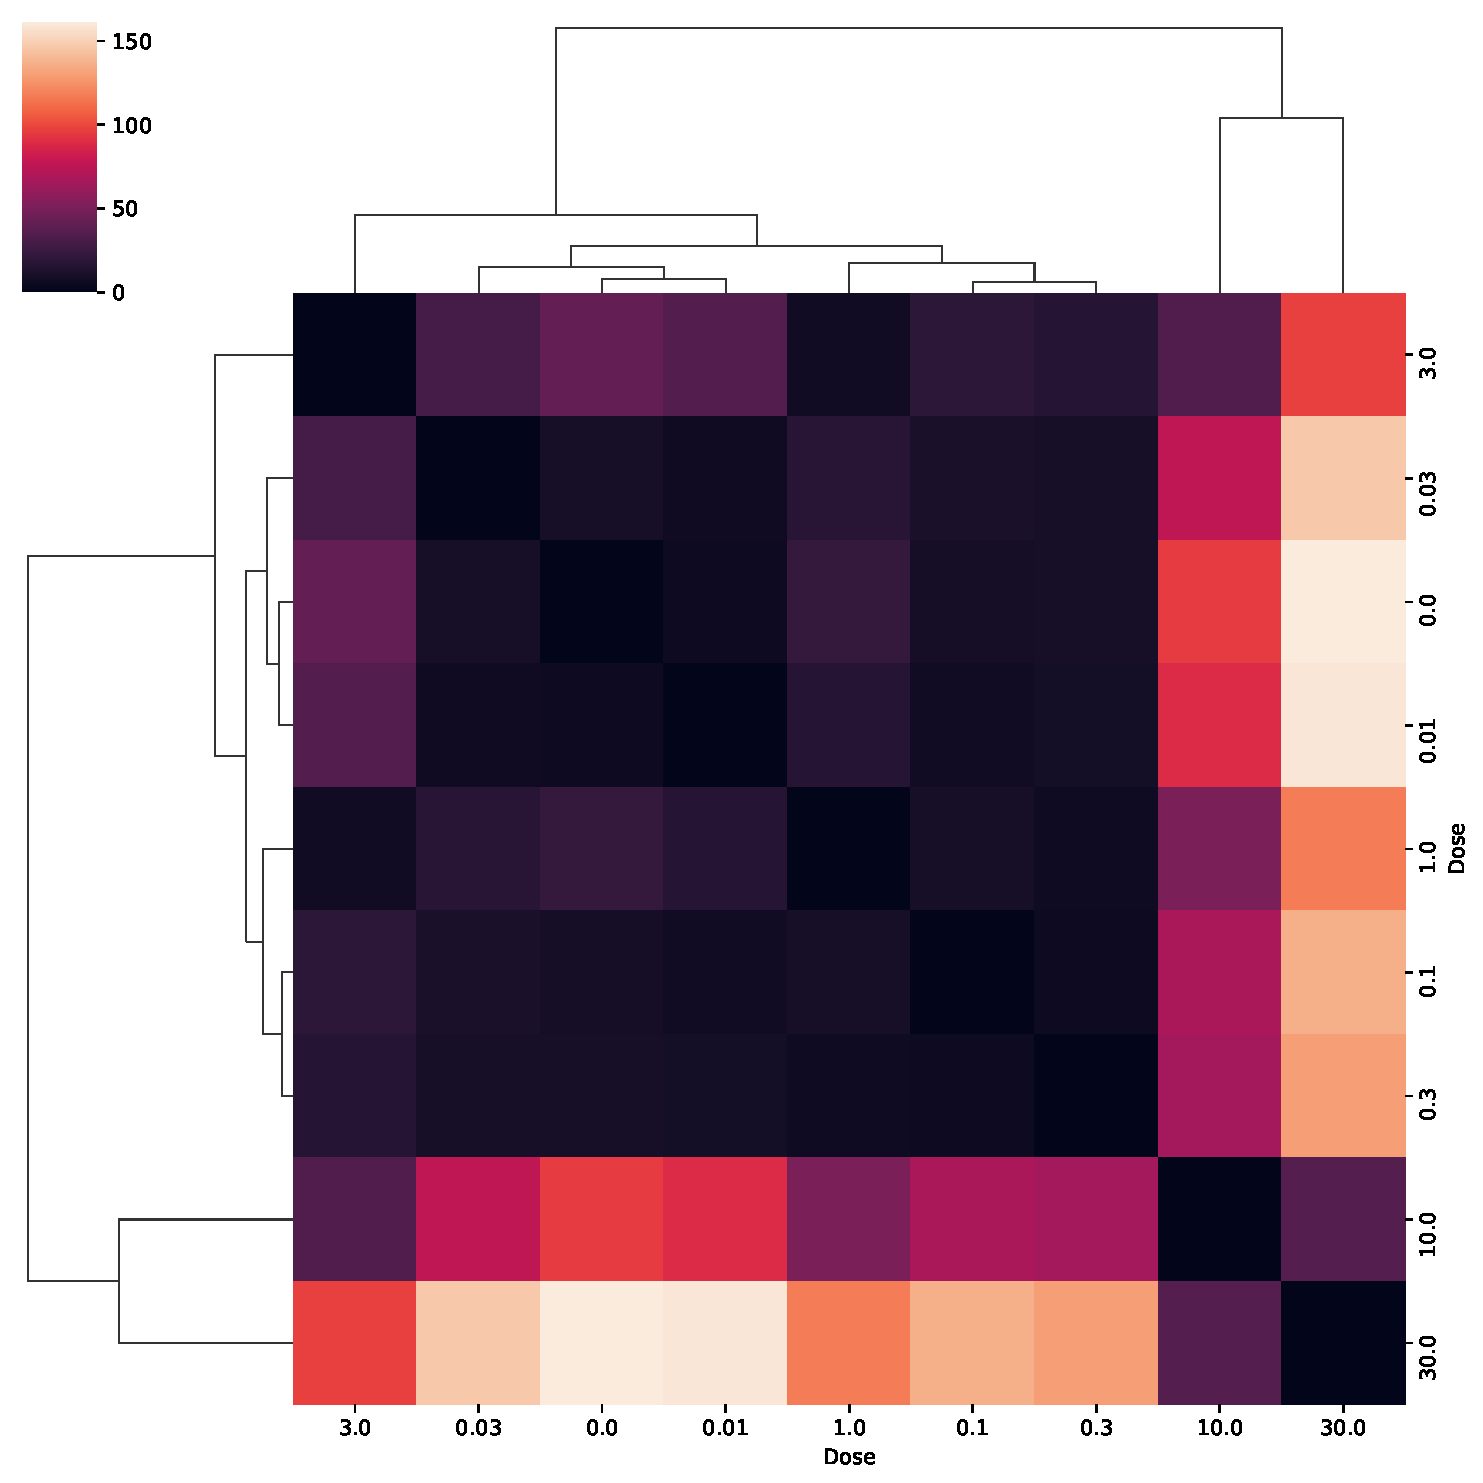
\includegraphics[width=\textwidth]{figures/hepatocytes_central_mmd_clustermap.pdf}
        \caption{MMD}
    \end{minipage}
    \vskip\baselineskip

    \begin{minipage}{0.4\textwidth}
        \centering
        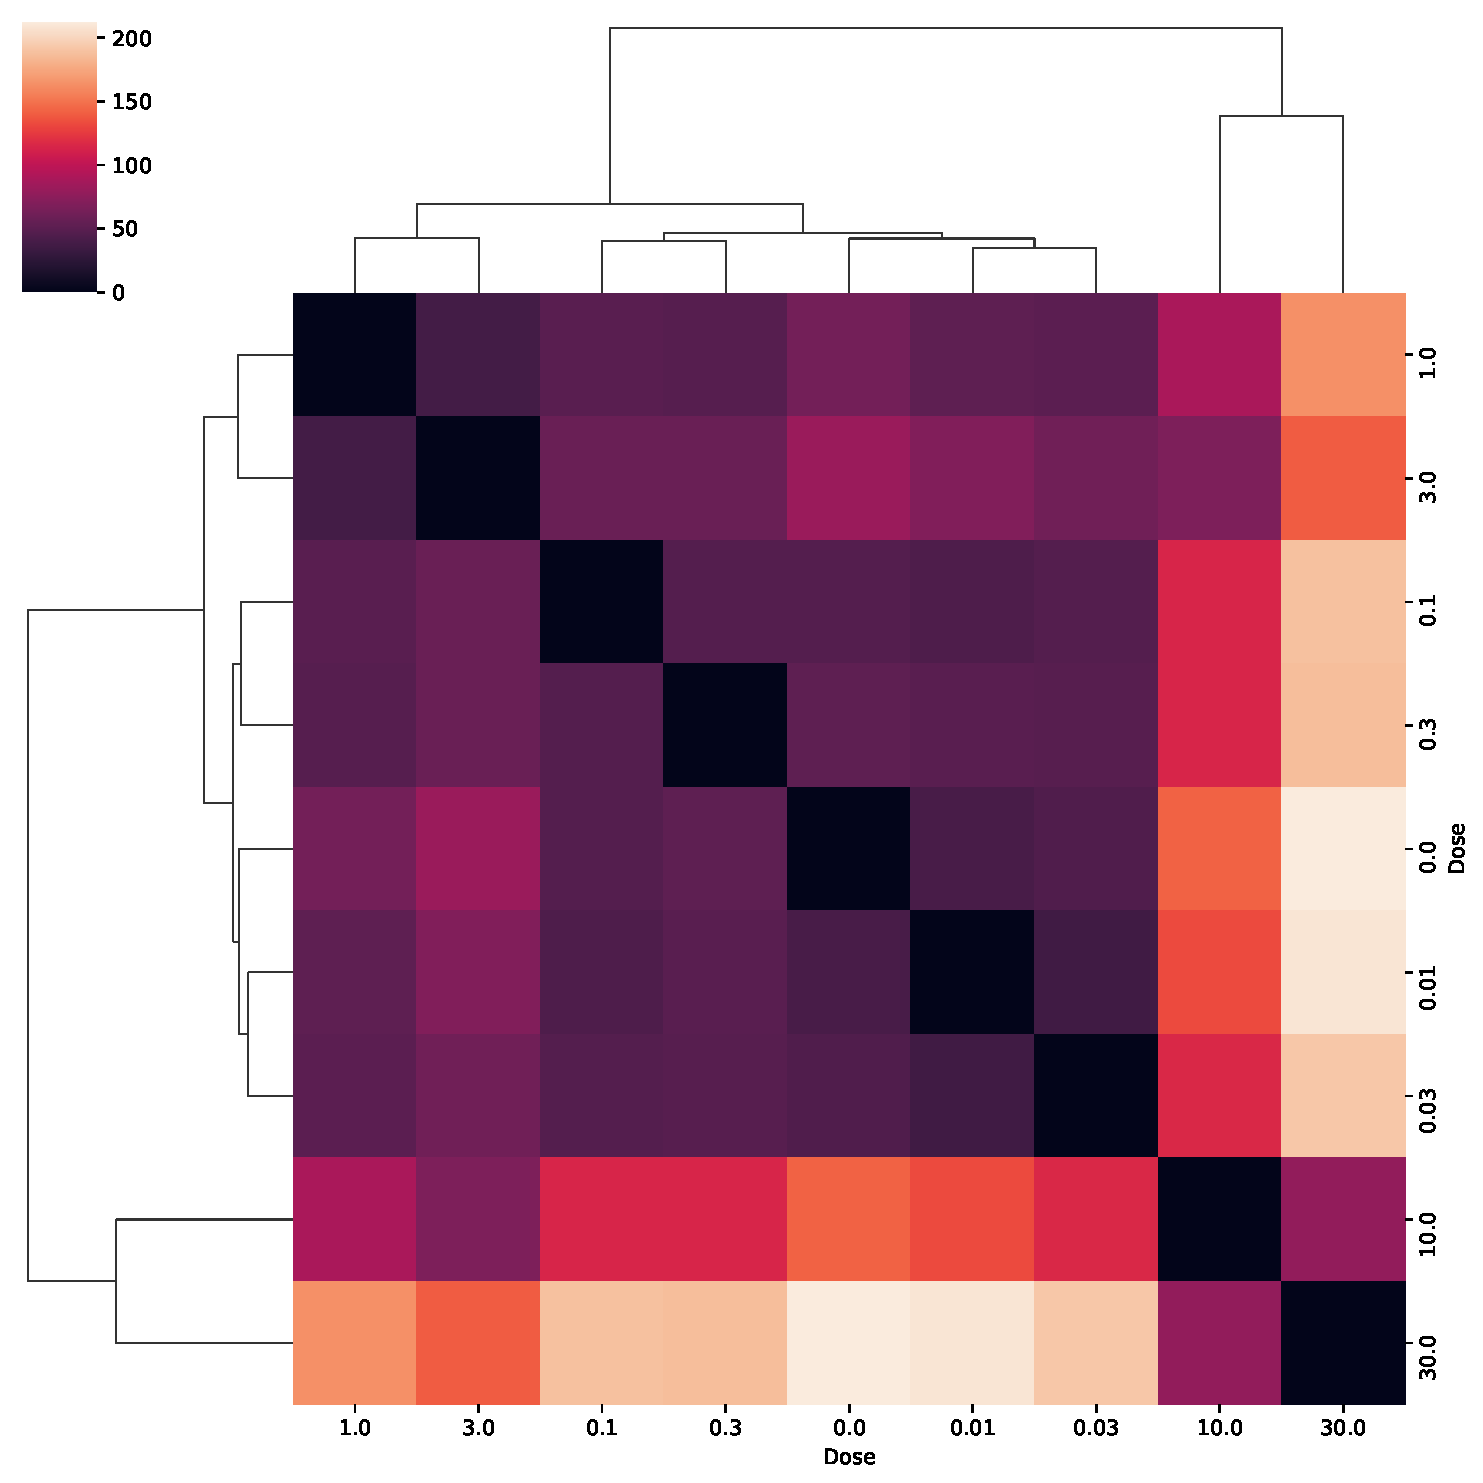
\includegraphics[width=\textwidth]{figures/hepatocytes_central_wasserstein_clustermap.pdf}
        \caption{Wasserstein}
    \end{minipage}
    \caption{Distance metrics for cell type Hepatocytes - central per dosage}
\end{figure}

\begin{figure}
    \centering
    \begin{minipage}{0.4\textwidth}
        \centering
        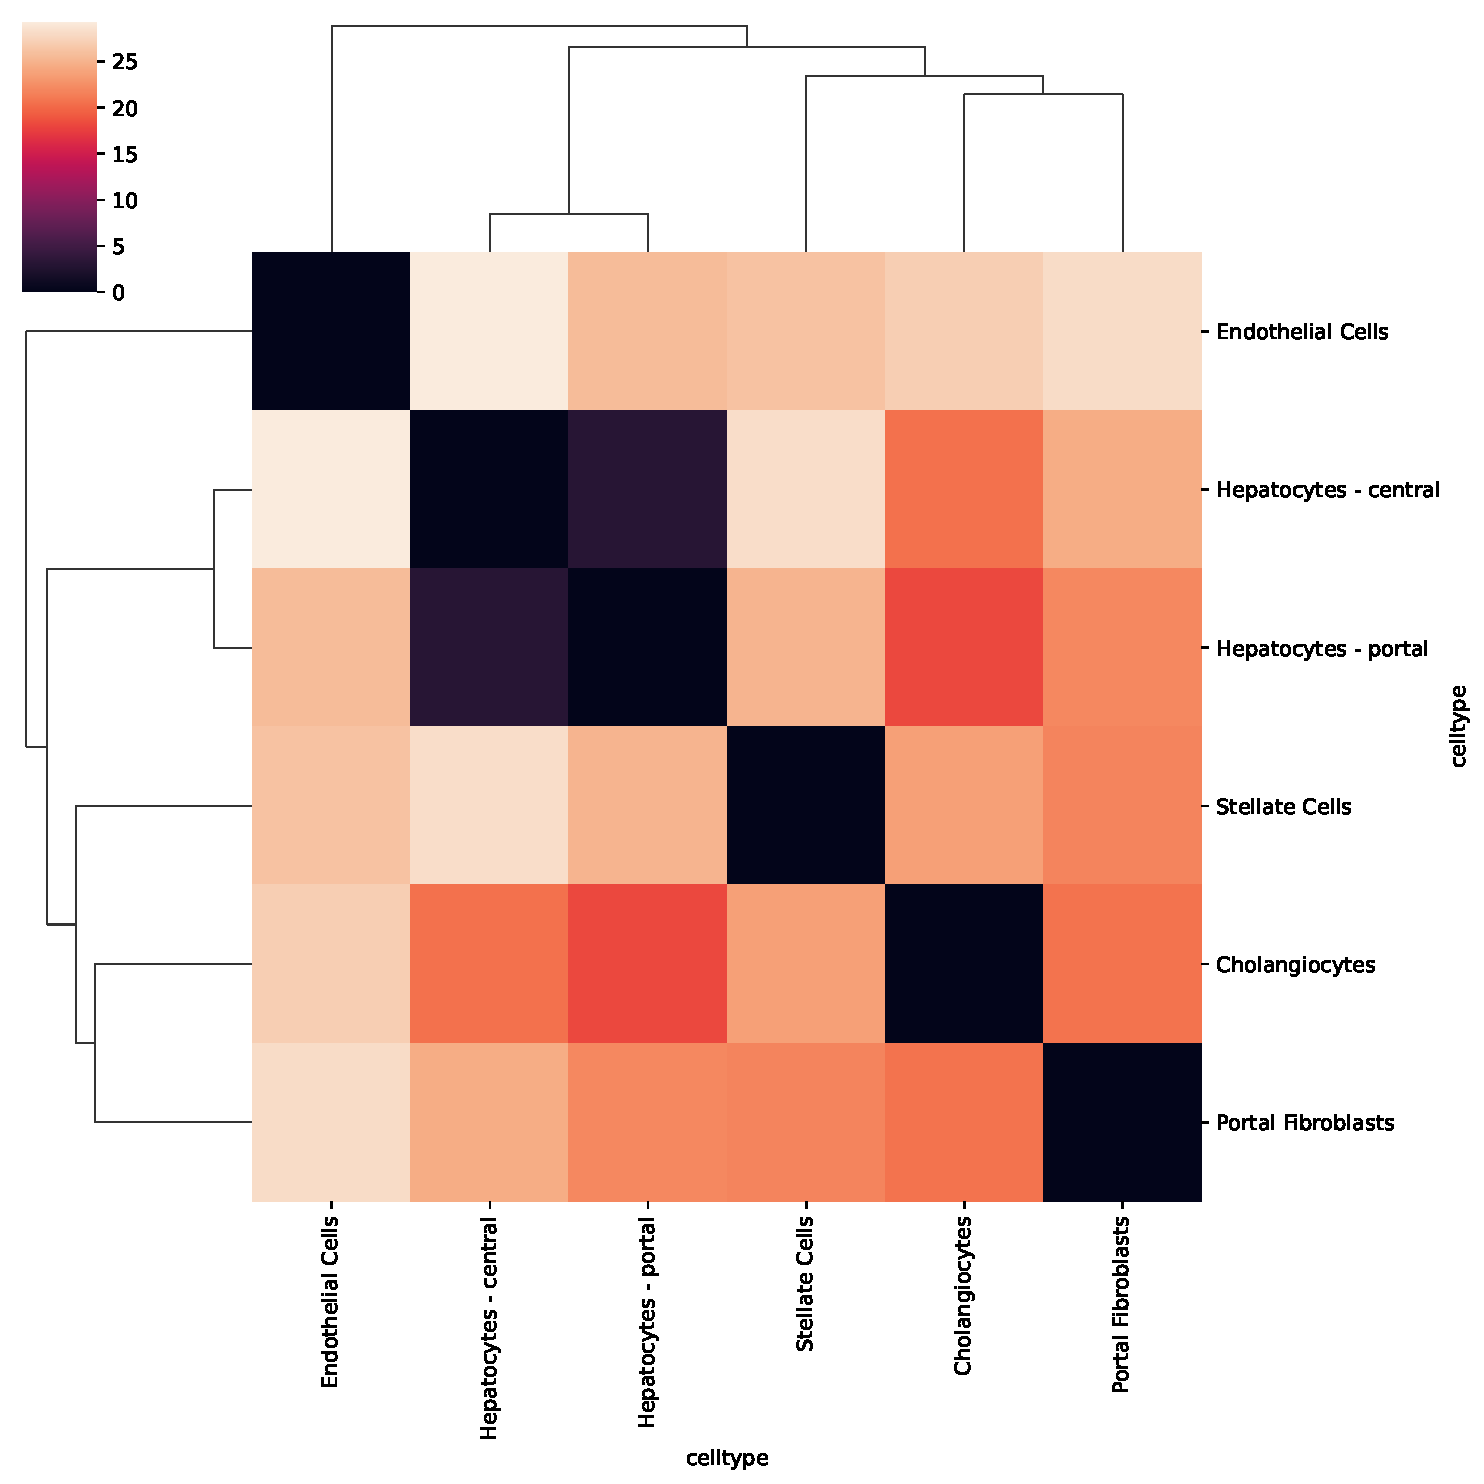
\includegraphics[width=\textwidth]{figures/dose_highest_edistance_clustermap.pdf}
        \caption{E-distance}
    \end{minipage} \hfill
    \begin{minipage}{0.4\textwidth}
        \centering
        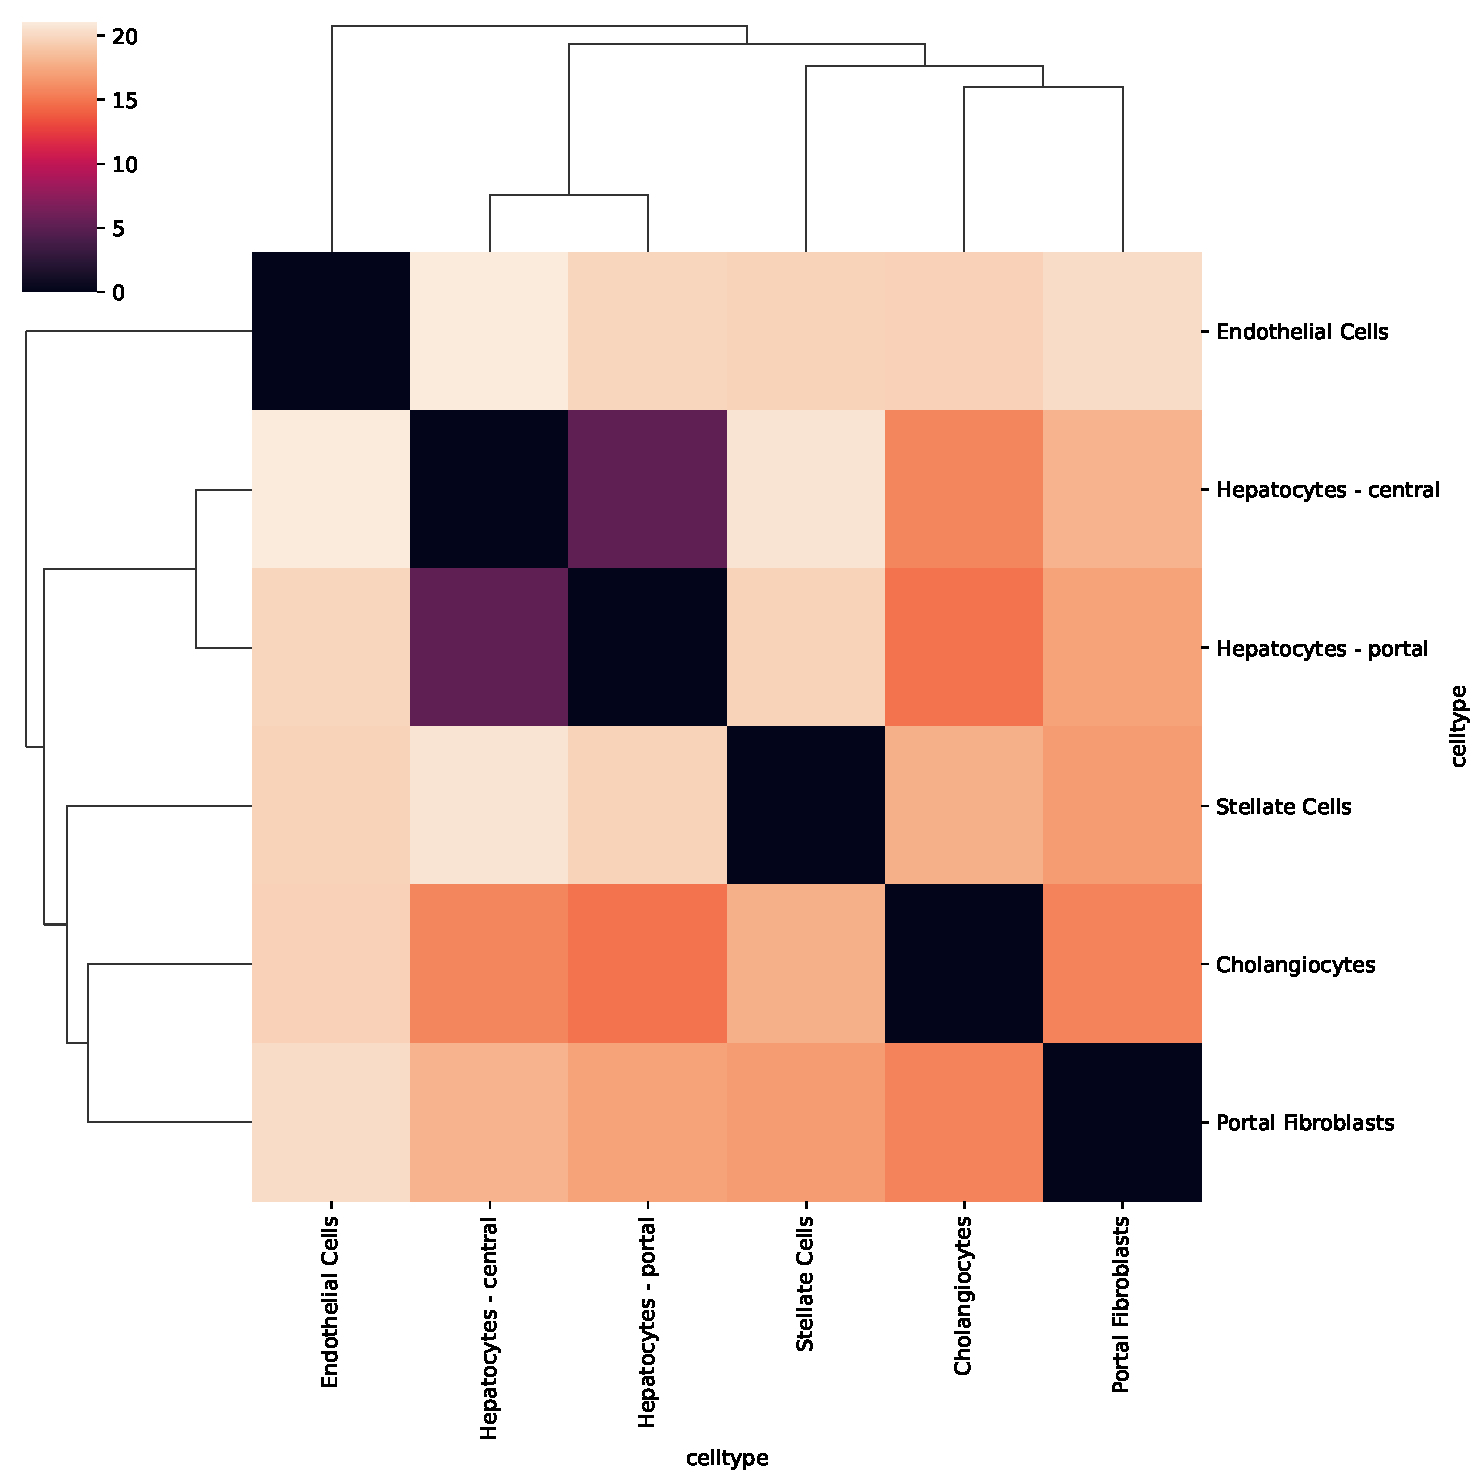
\includegraphics[width=\textwidth]{figures/dose_highest_euclidean_clustermap.pdf}
        \caption{Euclidean}
    \end{minipage}
    \vskip\baselineskip

    \begin{minipage}{0.4\textwidth}
        \centering
        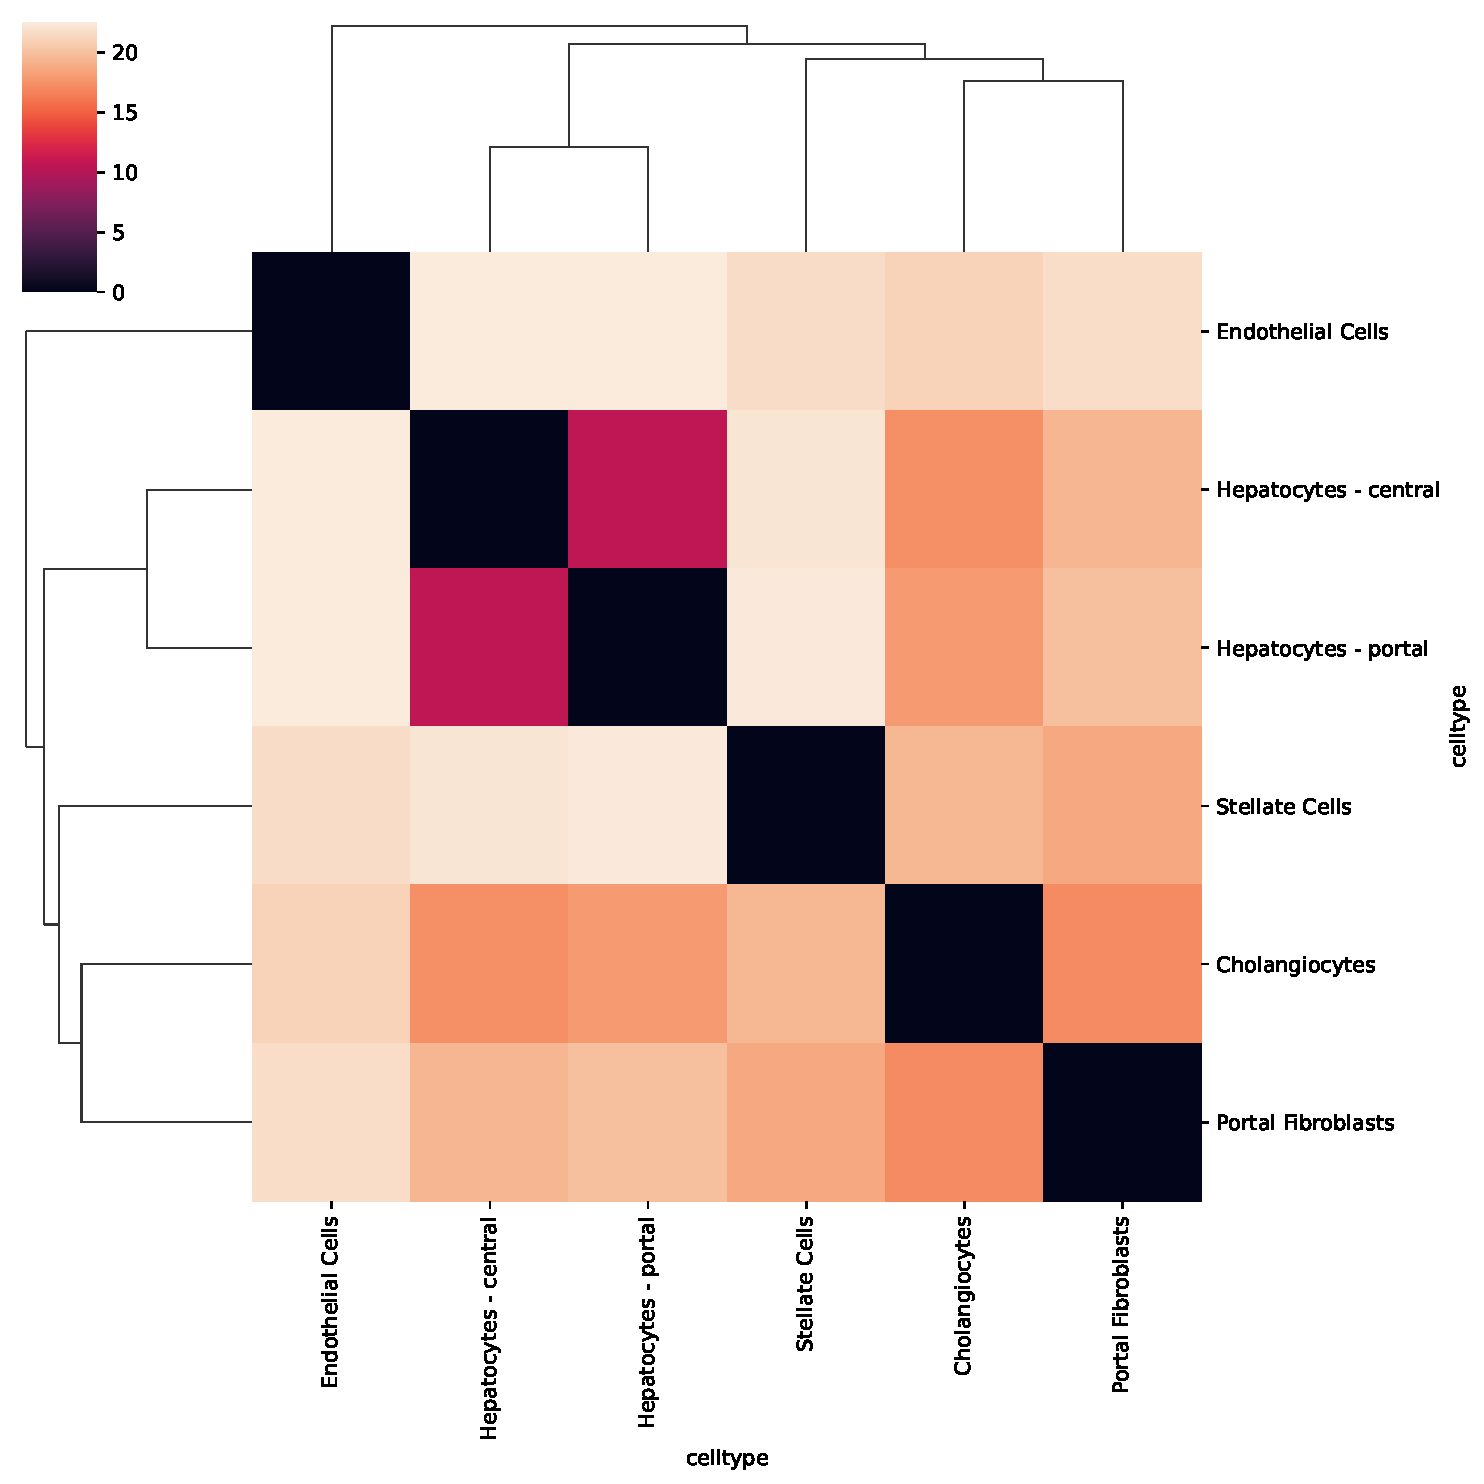
\includegraphics[width=\textwidth]{figures/dose_highest_mean_pairwise_clustermap.pdf}
        \caption{Mean pairwise}
    \end{minipage} \hfill
    \begin{minipage}{0.4\textwidth}
        \centering
        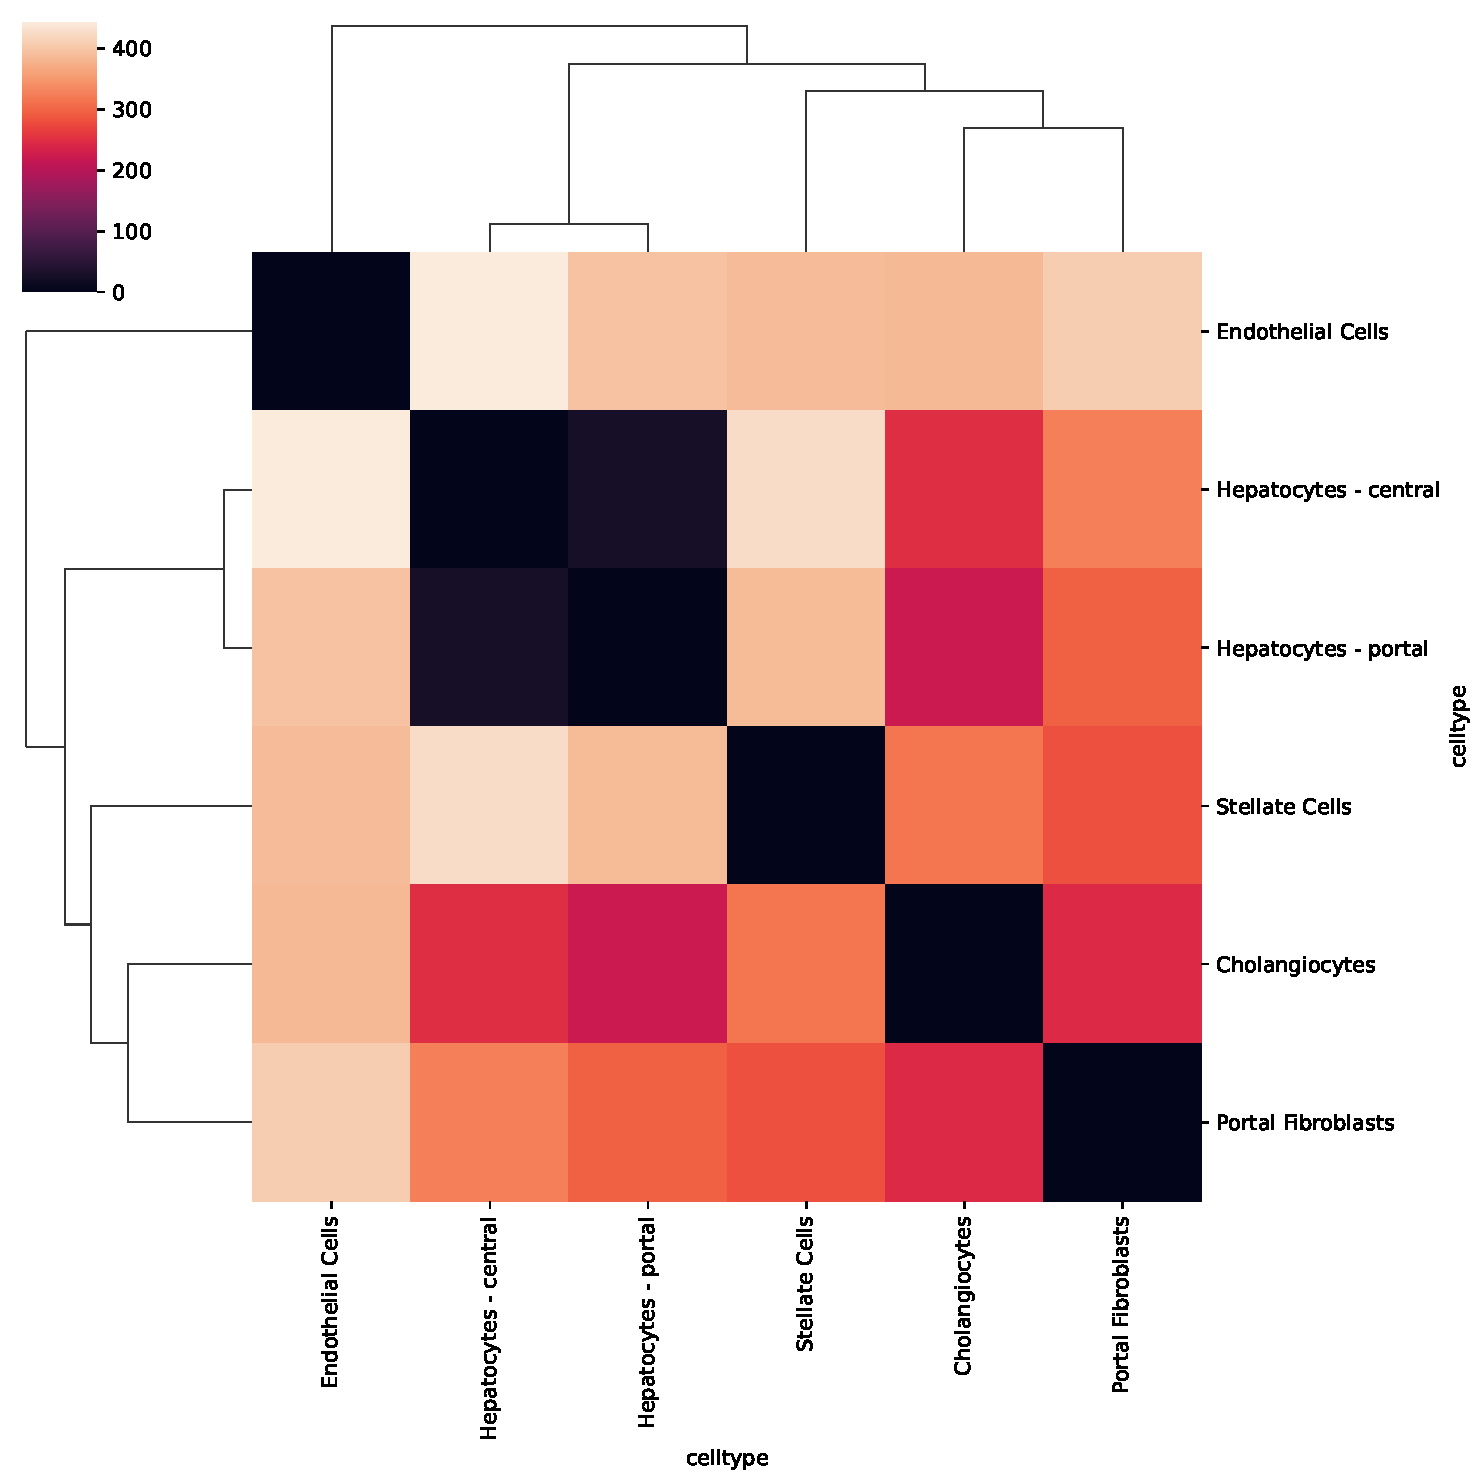
\includegraphics[width=\textwidth]{figures/dose_highest_mmd_clustermap.pdf}
        \caption{MMD}
    \end{minipage}
    \vskip\baselineskip

    \begin{minipage}{0.4\textwidth}
        \centering
        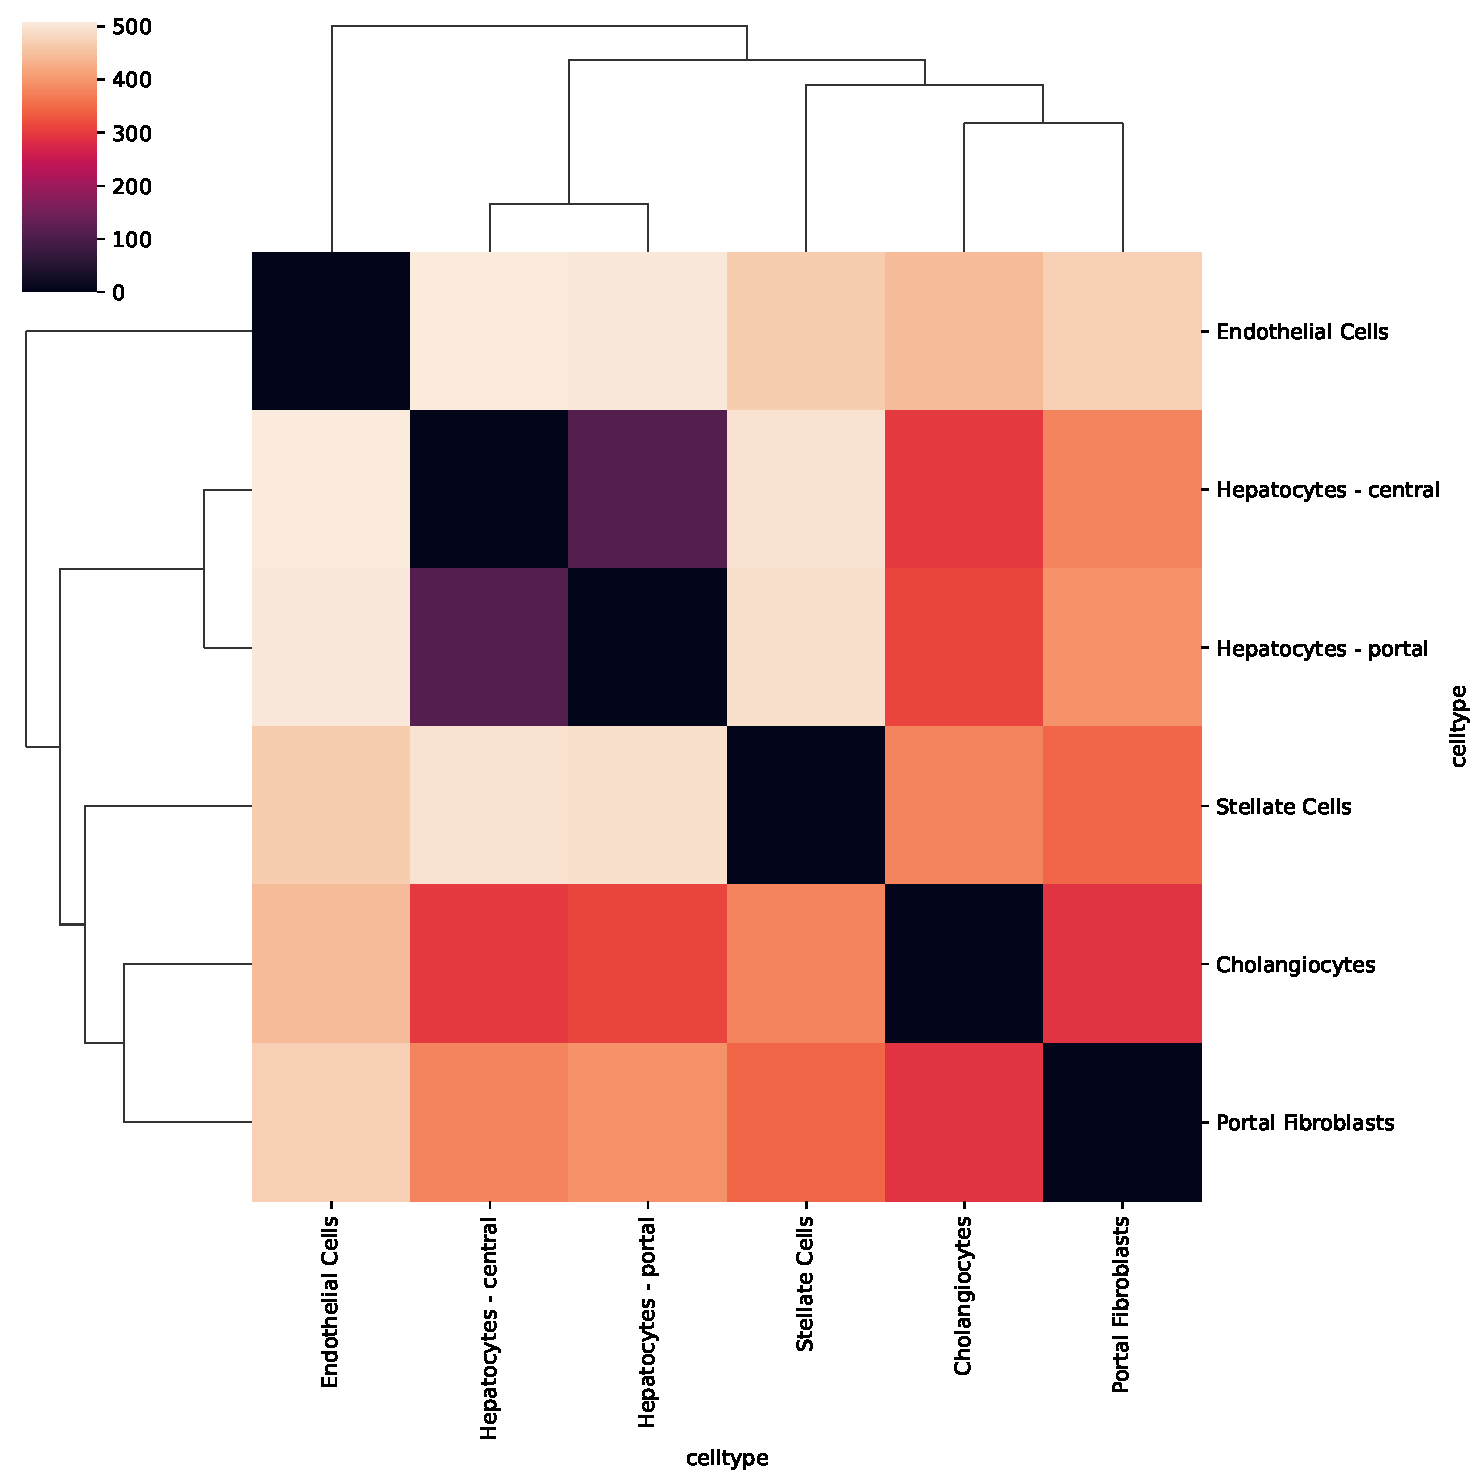
\includegraphics[width=\textwidth]{figures/dose_highest_wasserstein_clustermap.pdf}
        \caption{Wasserstein}
    \end{minipage}
    \caption{Distance metrics for dosage highest 30 $\mu g/kg$ per cell type}
\end{figure}

\begin{figure}
    \centering
    \begin{minipage}{0.4\textwidth}
        \centering
        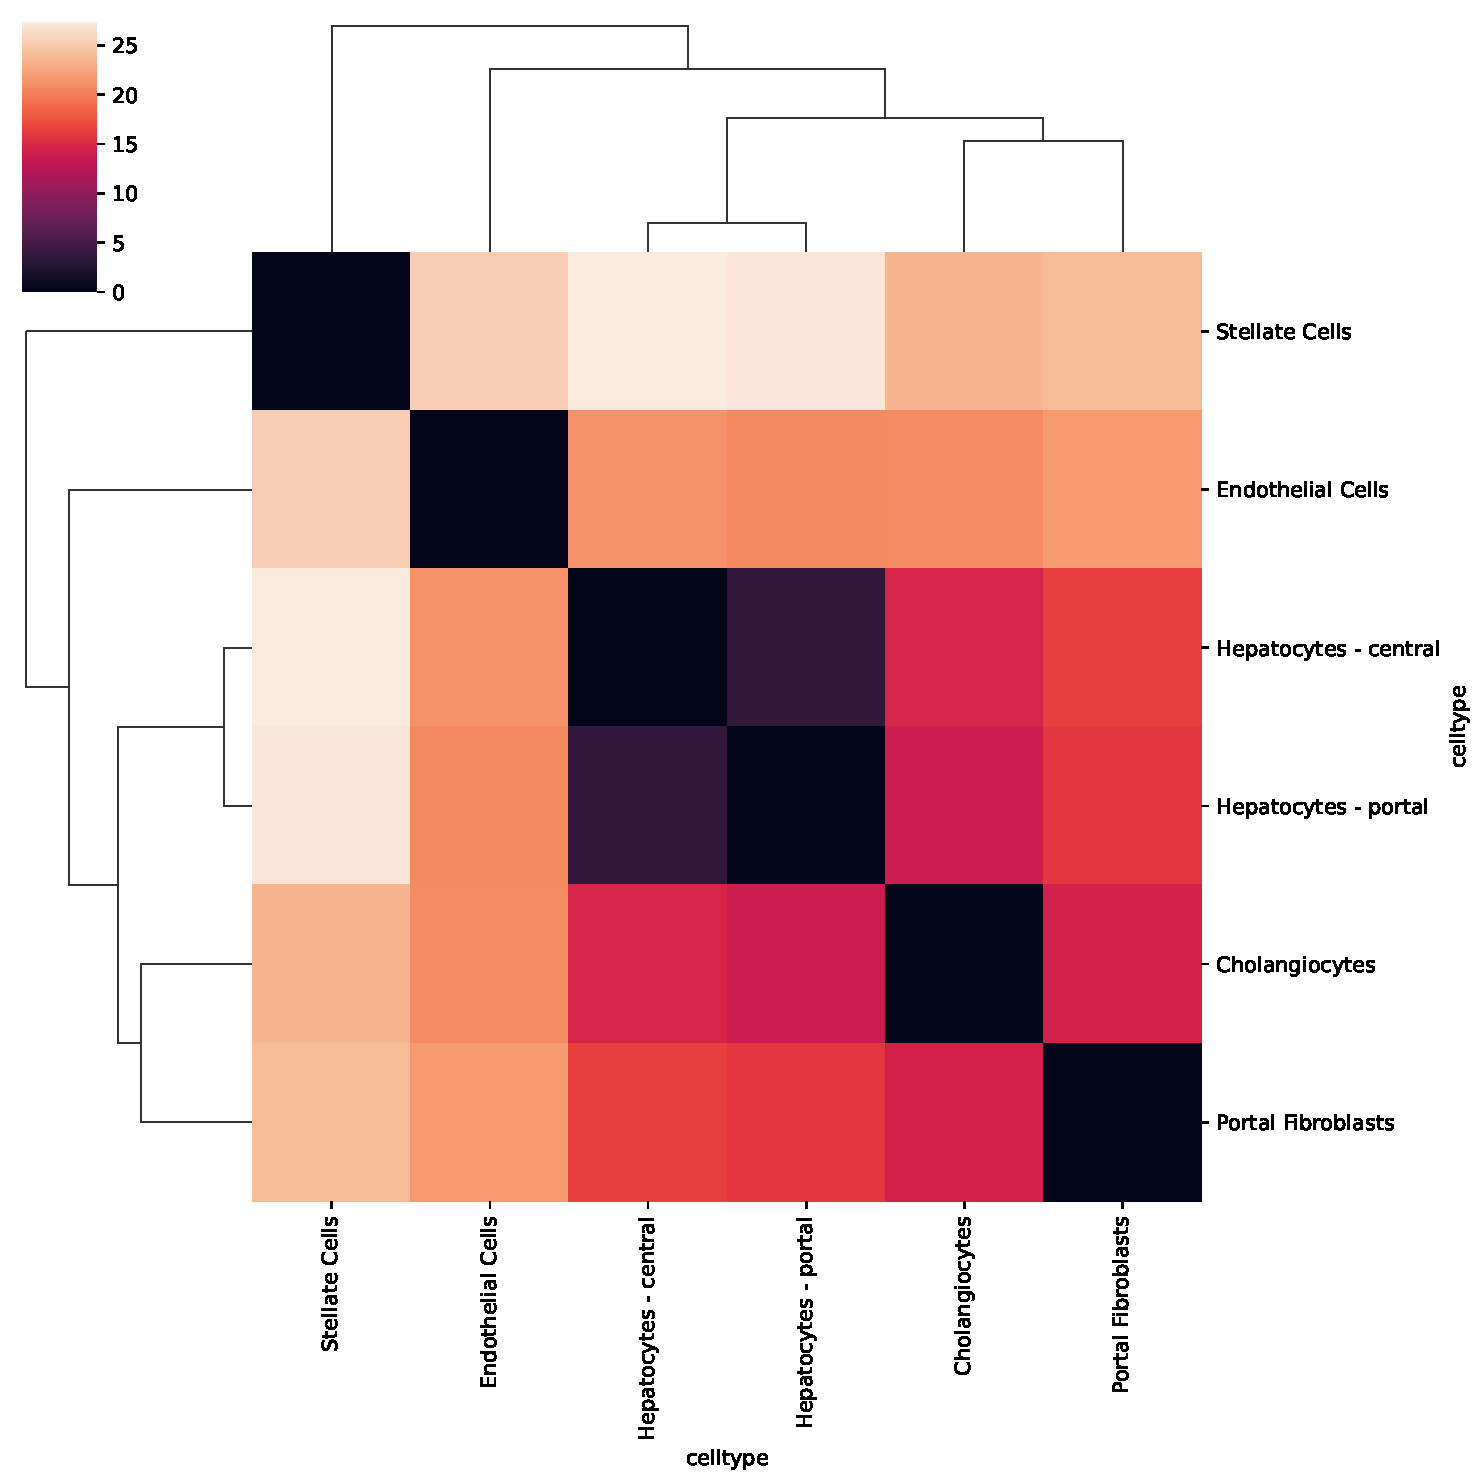
\includegraphics[width=\textwidth]{figures/dose_lowest_edistance_clustermap.pdf}
        \caption{E-distance}
    \end{minipage} \hfill
    \begin{minipage}{0.4\textwidth}
        \centering
        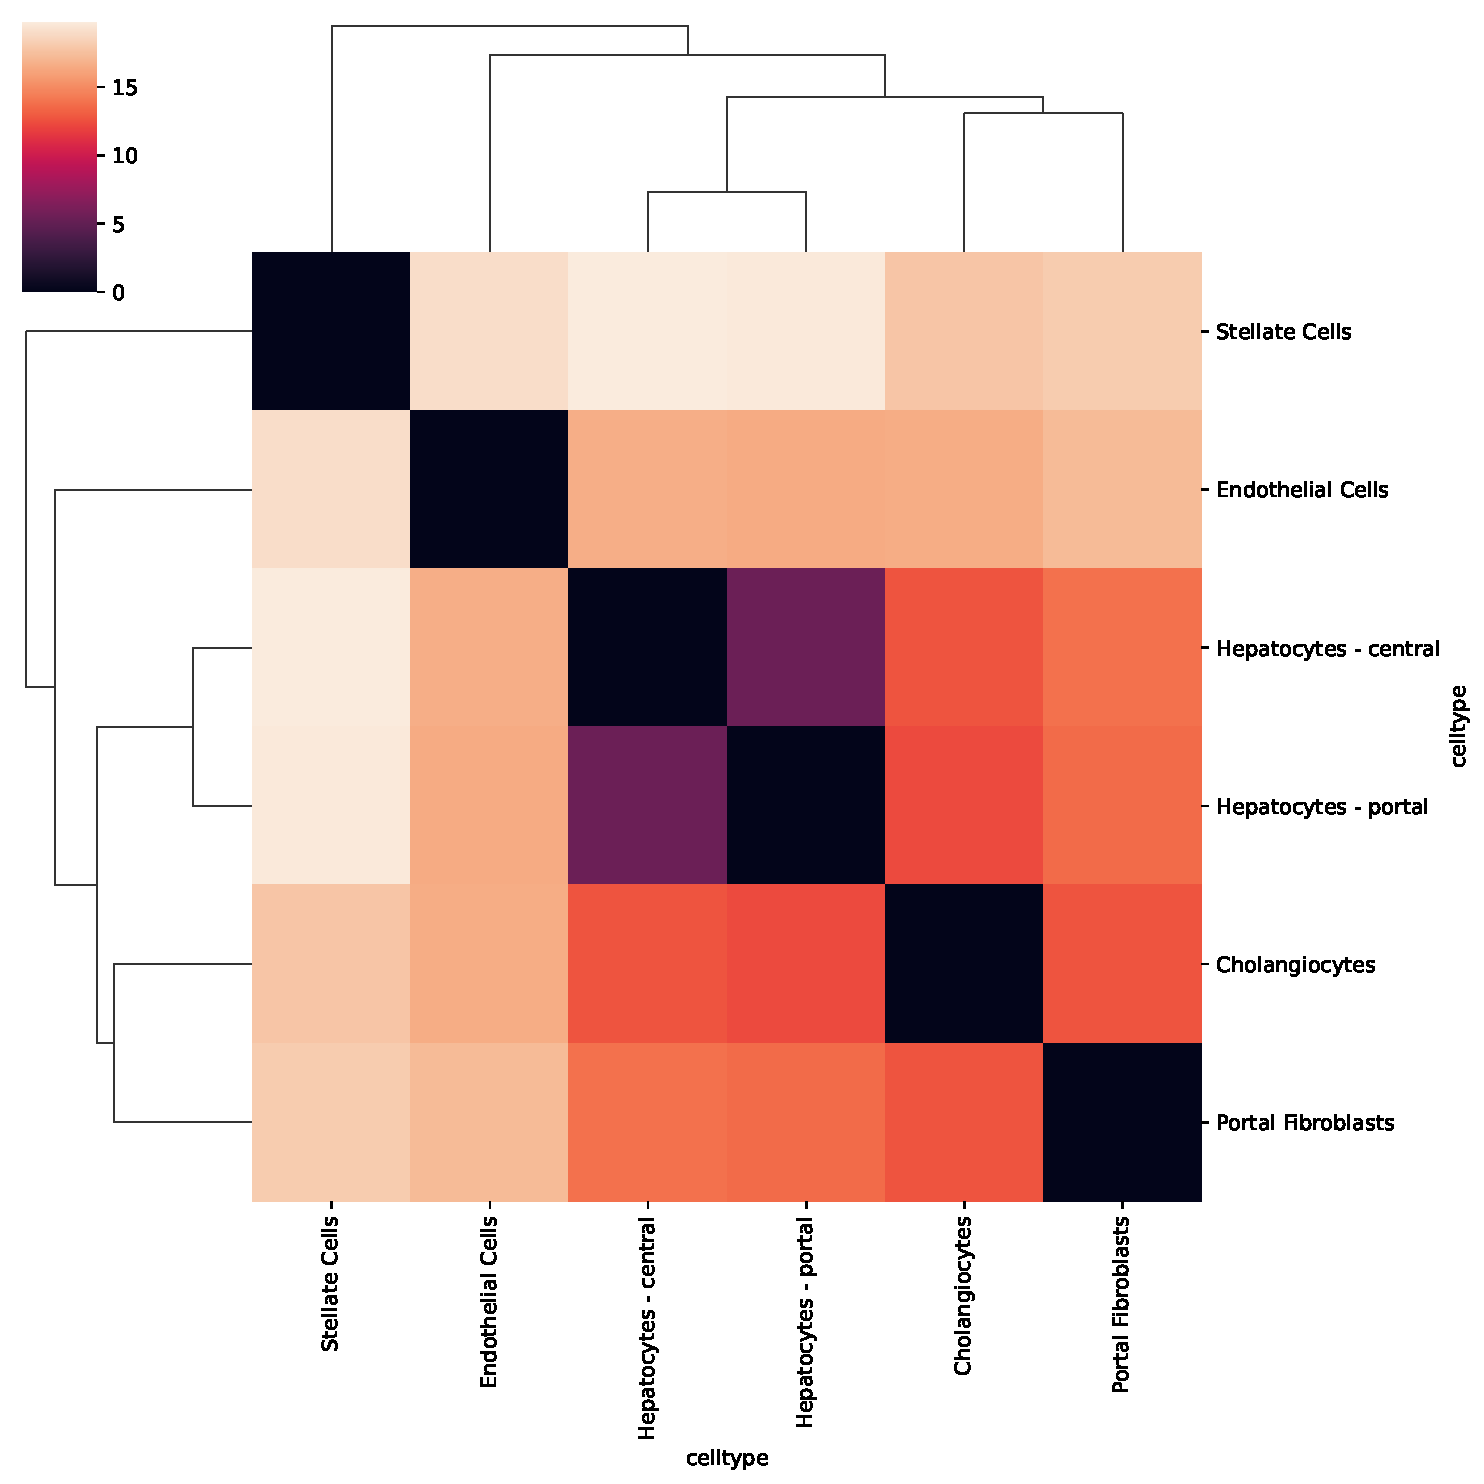
\includegraphics[width=\textwidth]{figures/dose_lowest_euclidean_clustermap.pdf}
        \caption{Euclidean}
    \end{minipage}
    \vskip\baselineskip

    \begin{minipage}{0.4\textwidth}
        \centering
        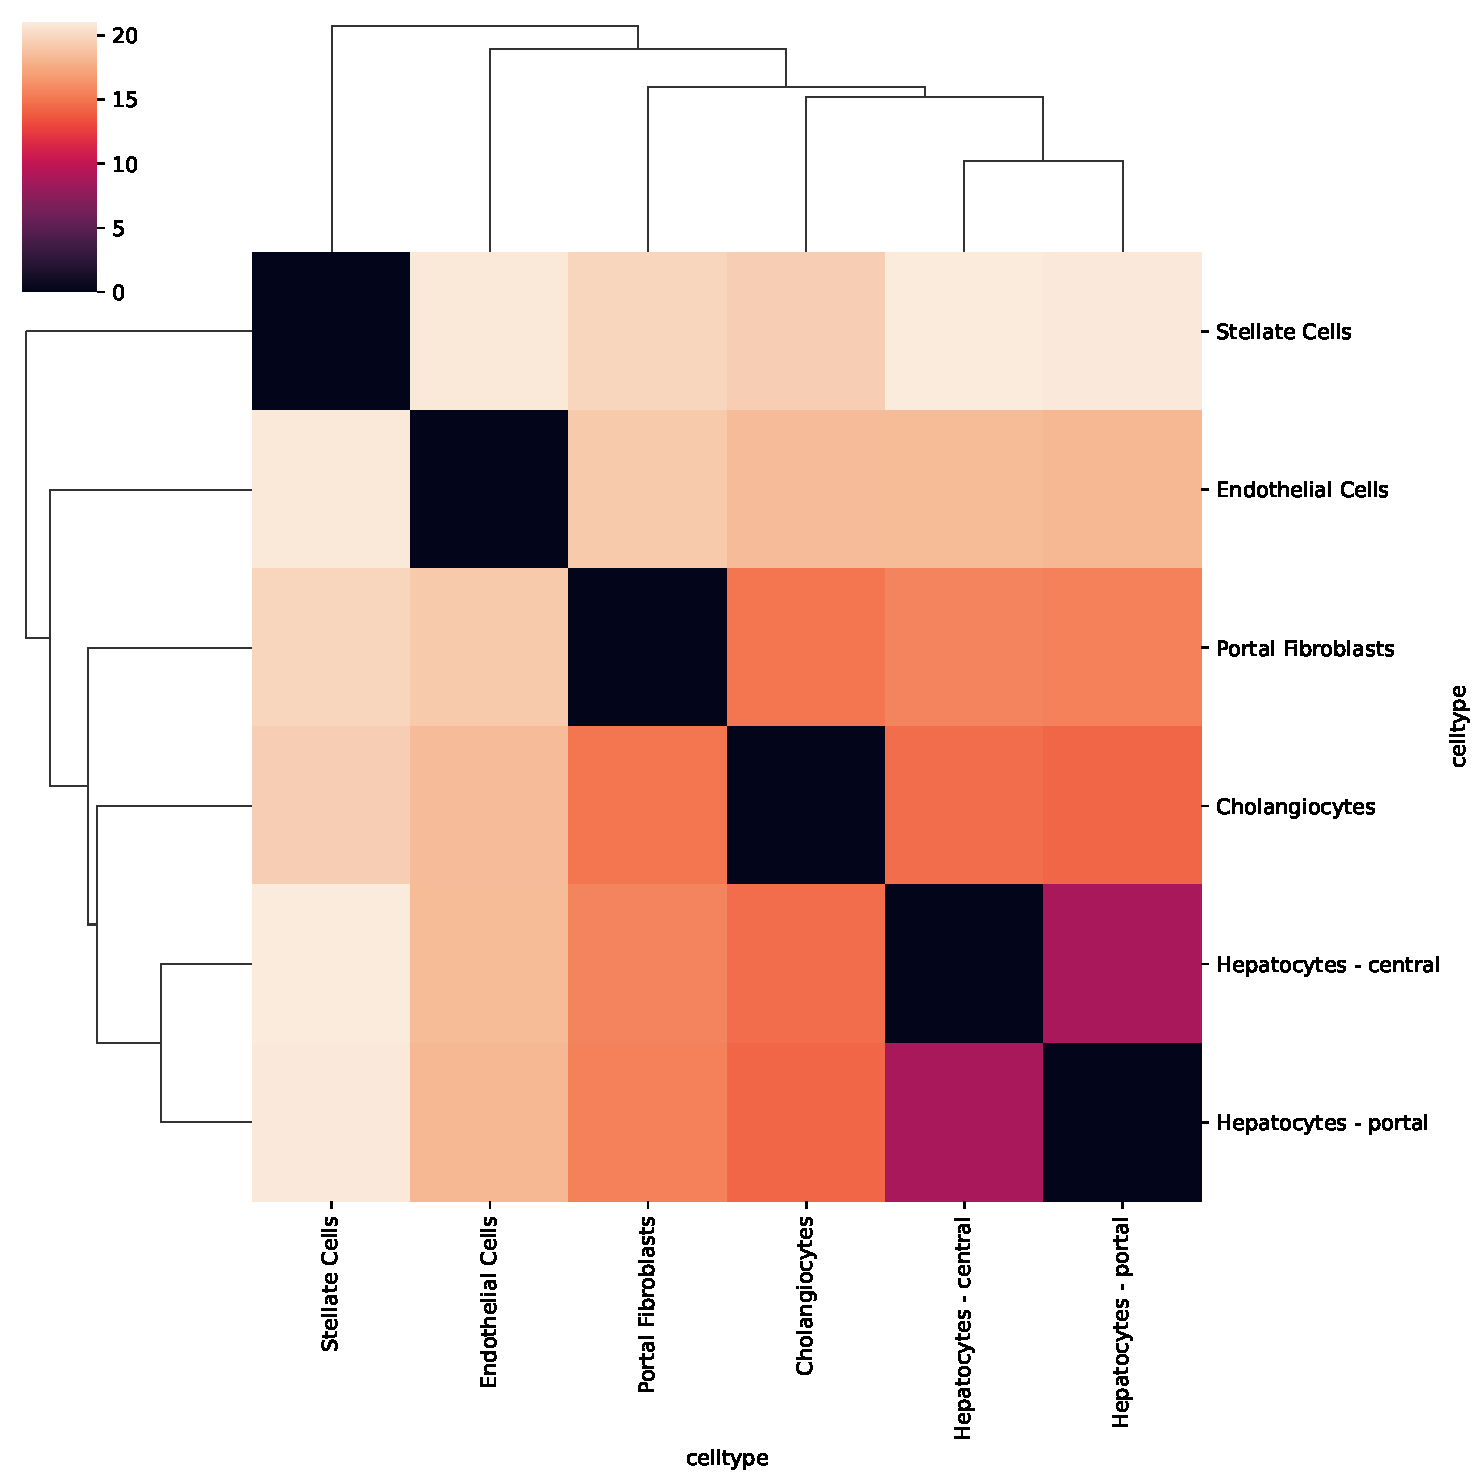
\includegraphics[width=\textwidth]{figures/dose_lowest_mean_pairwise_clustermap.pdf}
        \caption{Mean pairwise}
    \end{minipage} \hfill
    \begin{minipage}{0.4\textwidth}
        \centering
        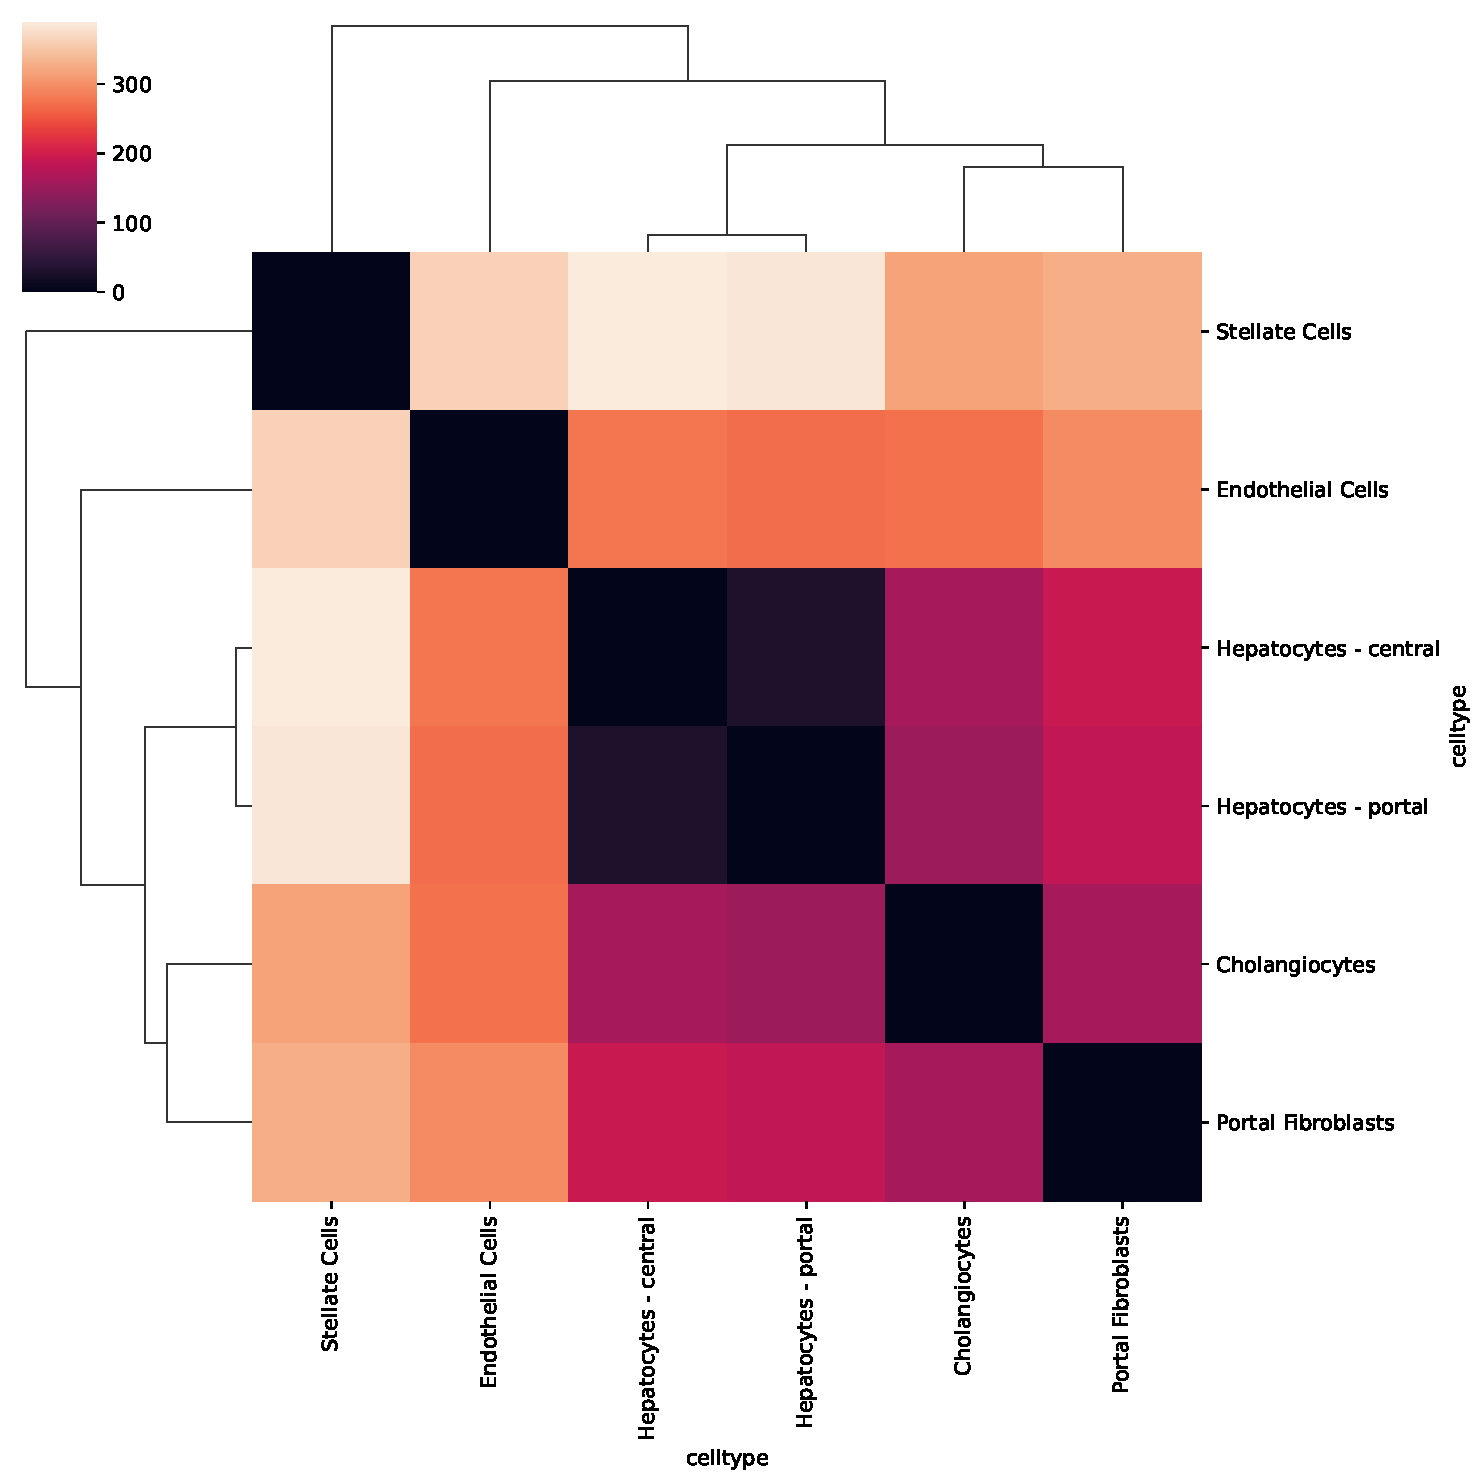
\includegraphics[width=\textwidth]{figures/dose_lowest_mmd_clustermap.pdf}
        \caption{MMD}
    \end{minipage}
    \vskip\baselineskip

    \begin{minipage}{0.4\textwidth}
        \centering
        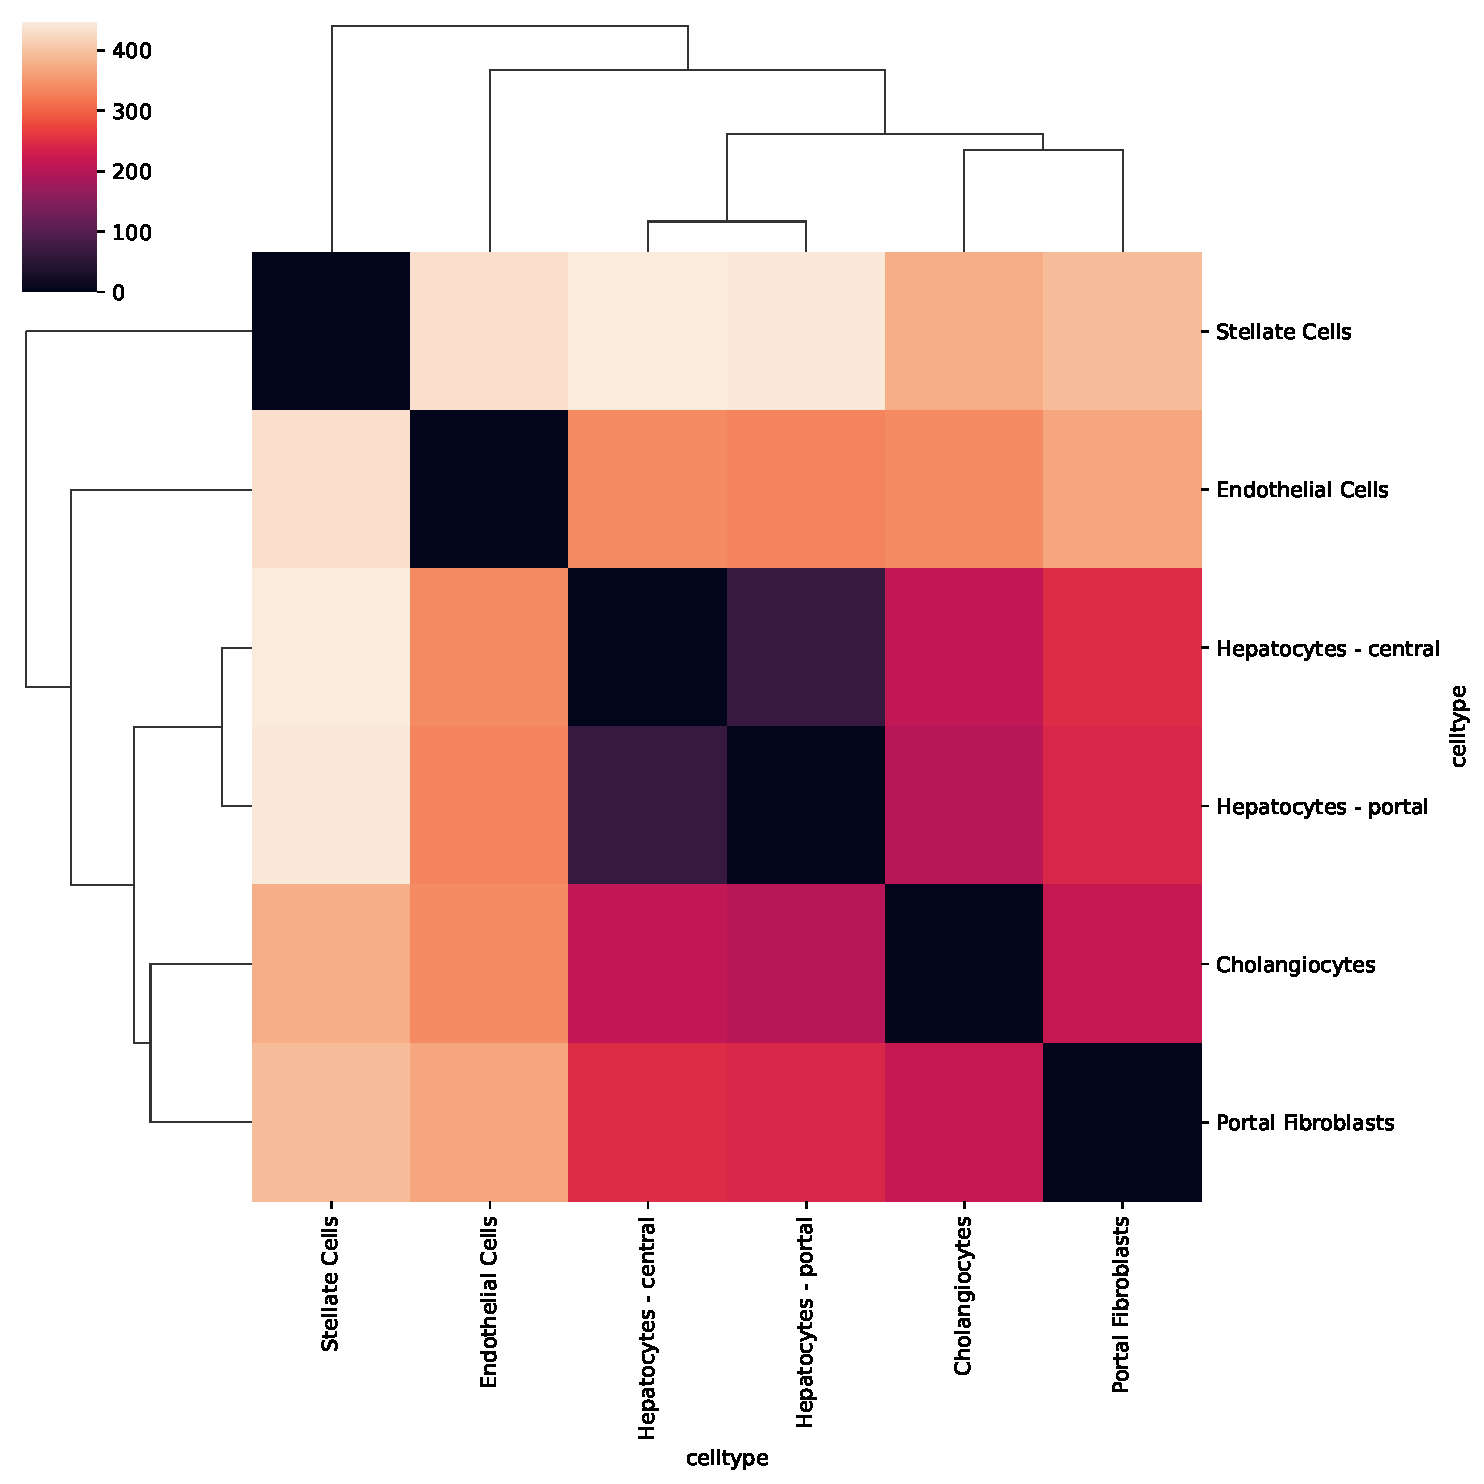
\includegraphics[width=\textwidth]{figures/dose_lowest_wasserstein_clustermap.pdf}
        \caption{Wasserstein}
    \end{minipage}
    \caption{Distance metrics for lowest dosage 0.01 $\mu g/kg$ per cell type}
\end{figure}

\clearpage


\subsection{PBMC dataset}


\begin{figure}[h]
    \centering
    \begin{subfigure}[t]{0.49\textwidth}
        \centering
        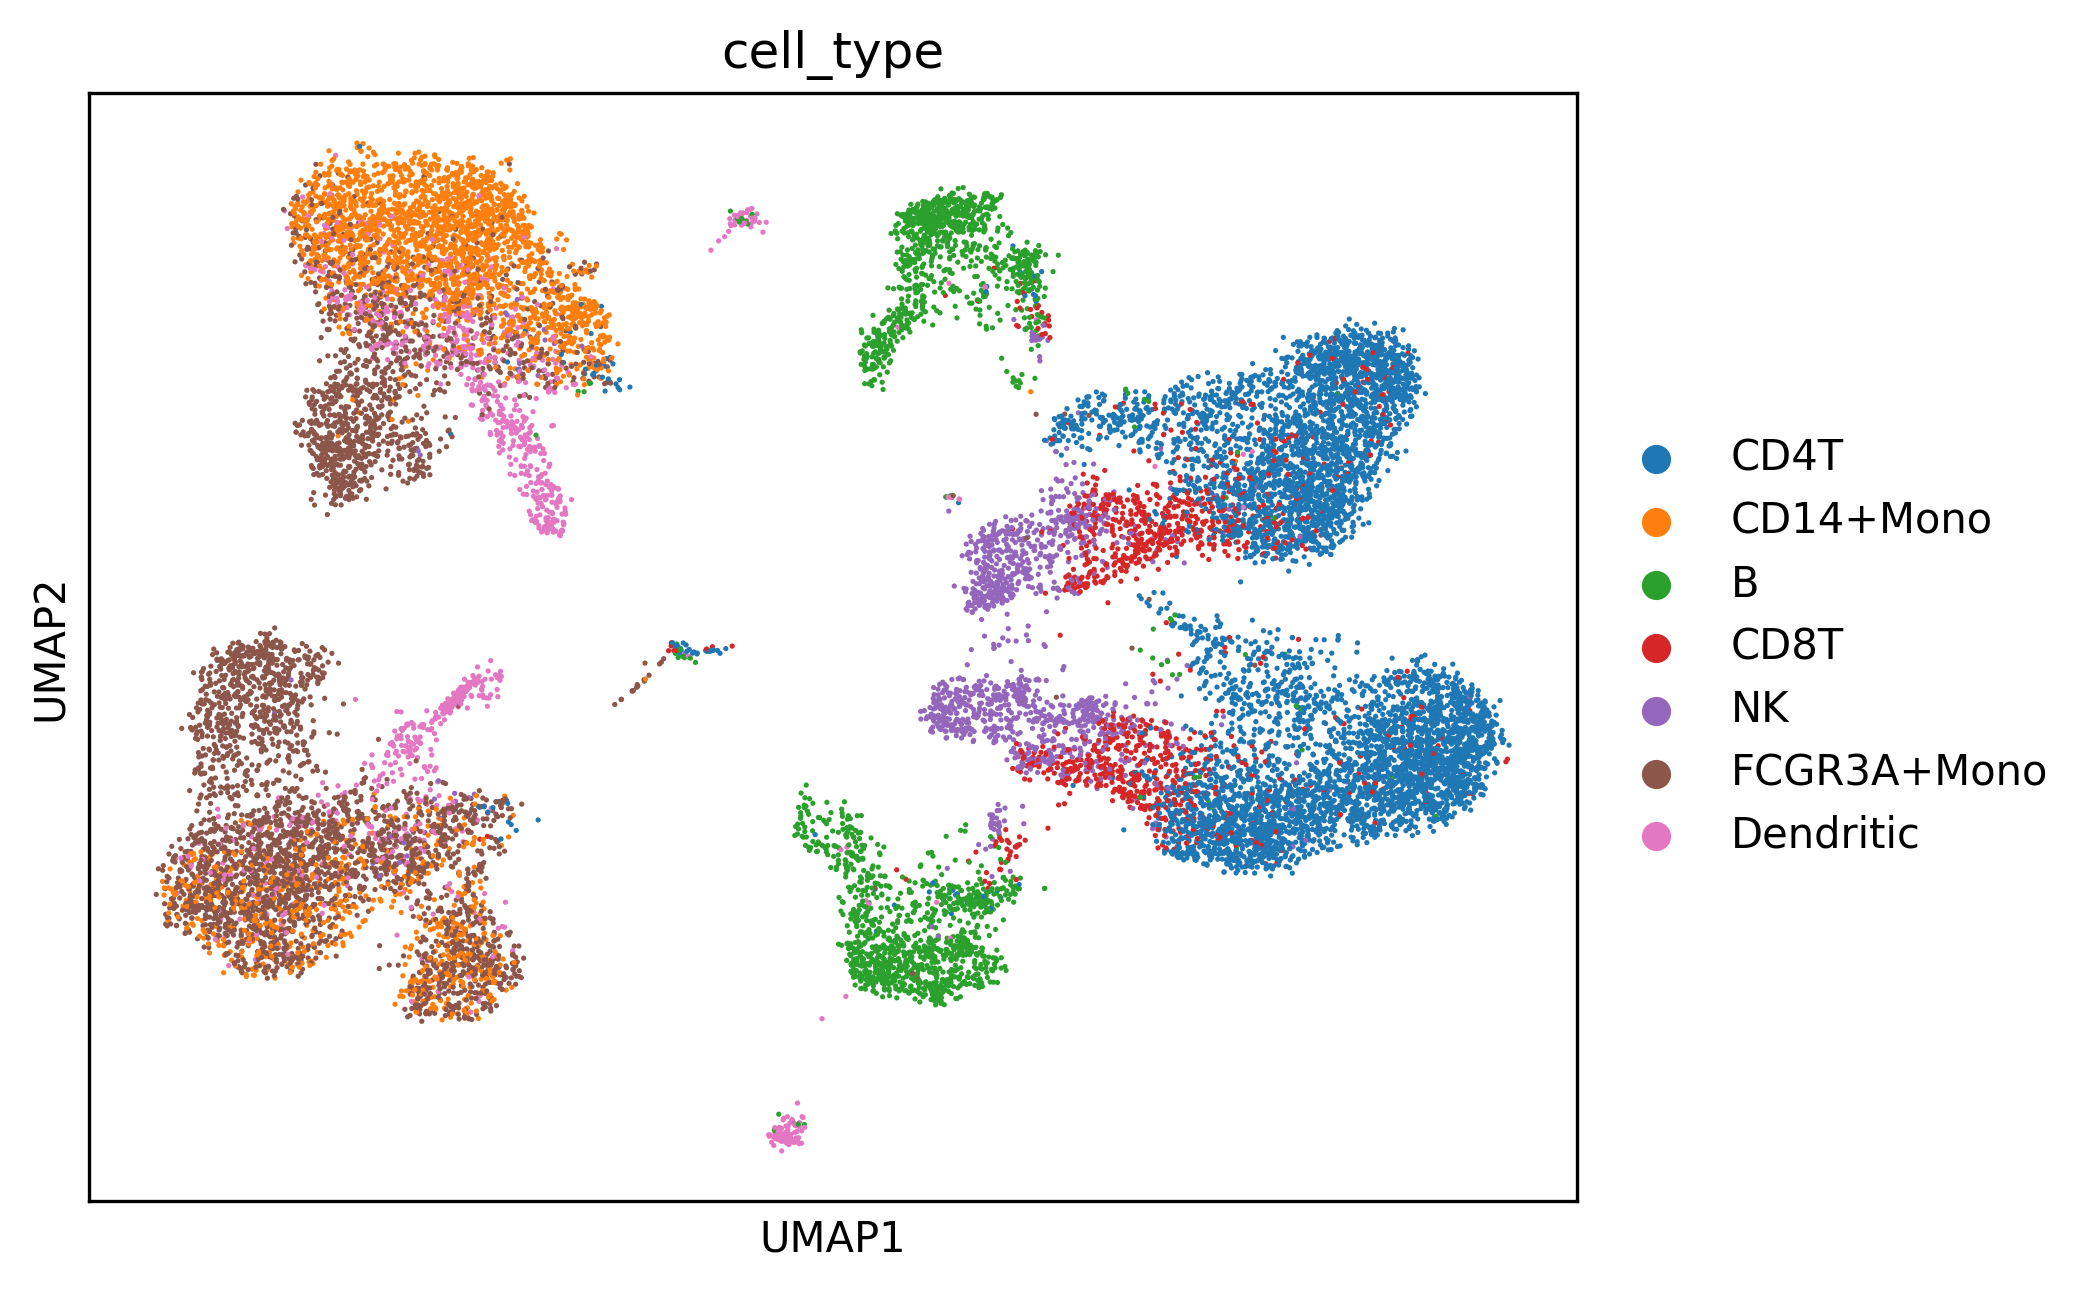
\includegraphics[width=\textwidth]{figures/pbmc_cell_umap.png}
        \caption{}
        \label{fig:figure1}
    \end{subfigure}
    \hfill
    \begin{subfigure}[t]{0.49\textwidth}
        \centering
        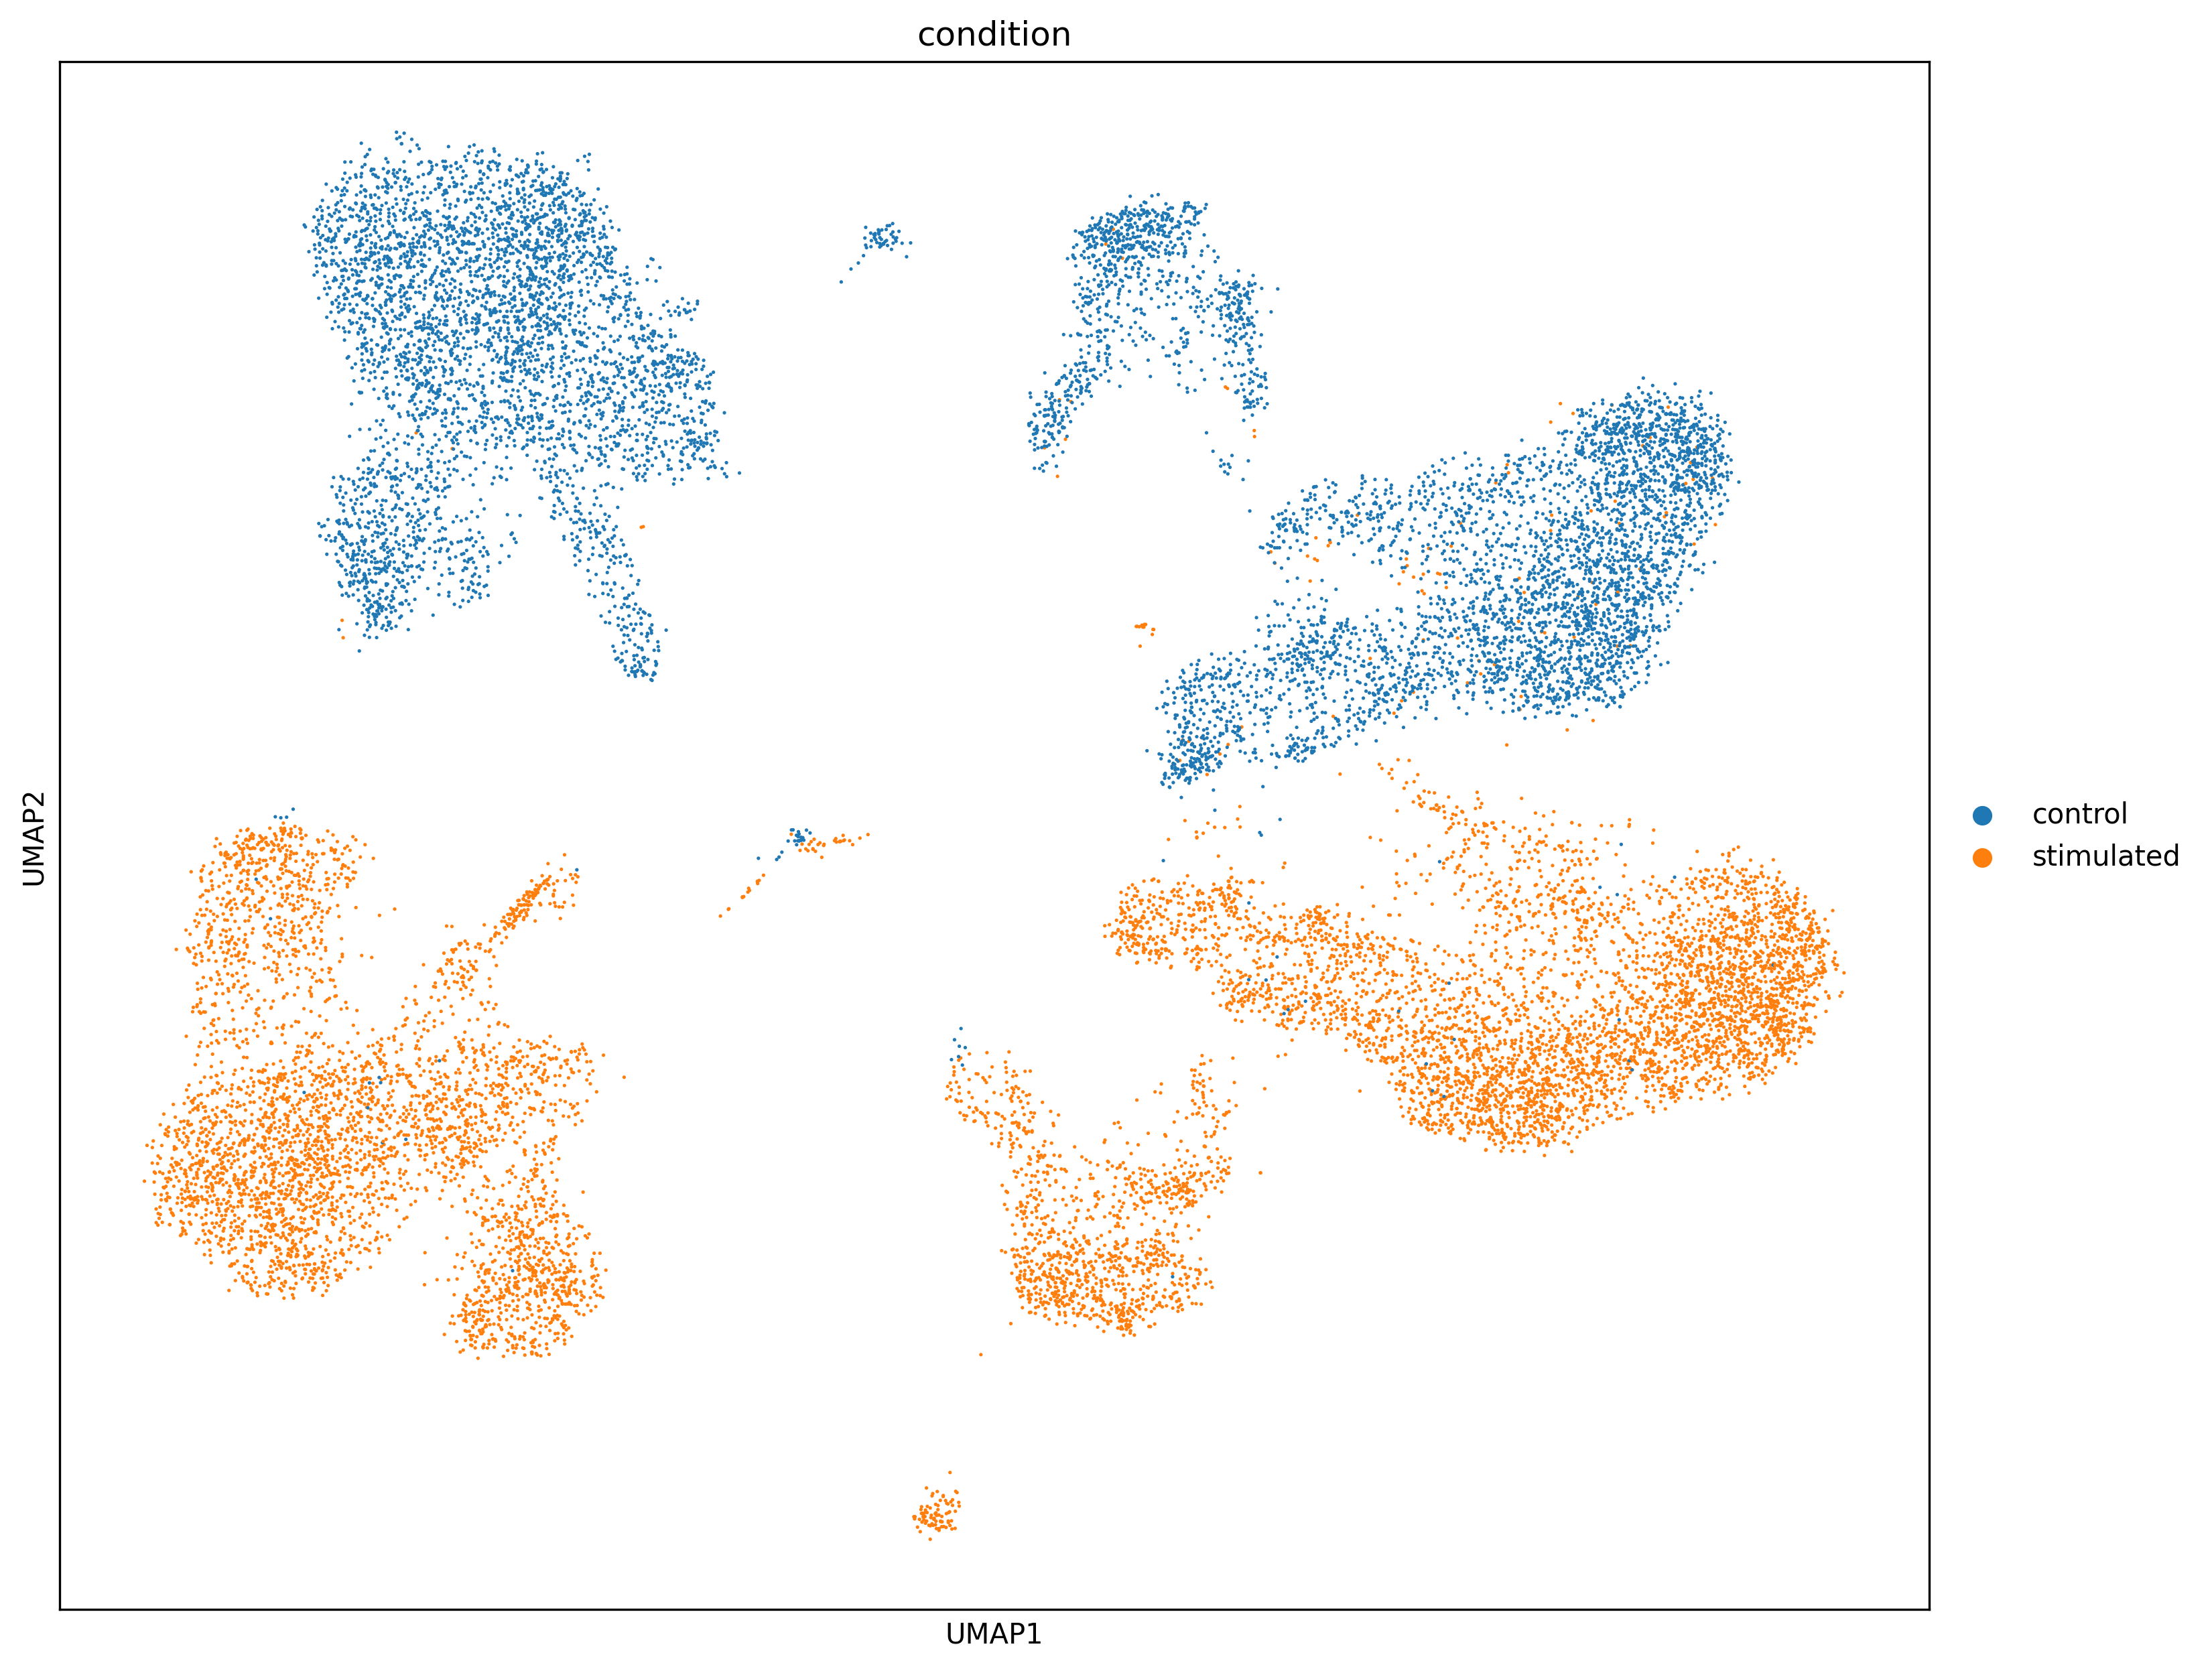
\includegraphics[width=.95\textwidth]{figures/pbmc_condtion_umap.png}
        \caption{}
        \label{fig:figure2}
    \end{subfigure}
    \hfill
    \begin{subfigure}[b]{\textwidth}
        \centering
        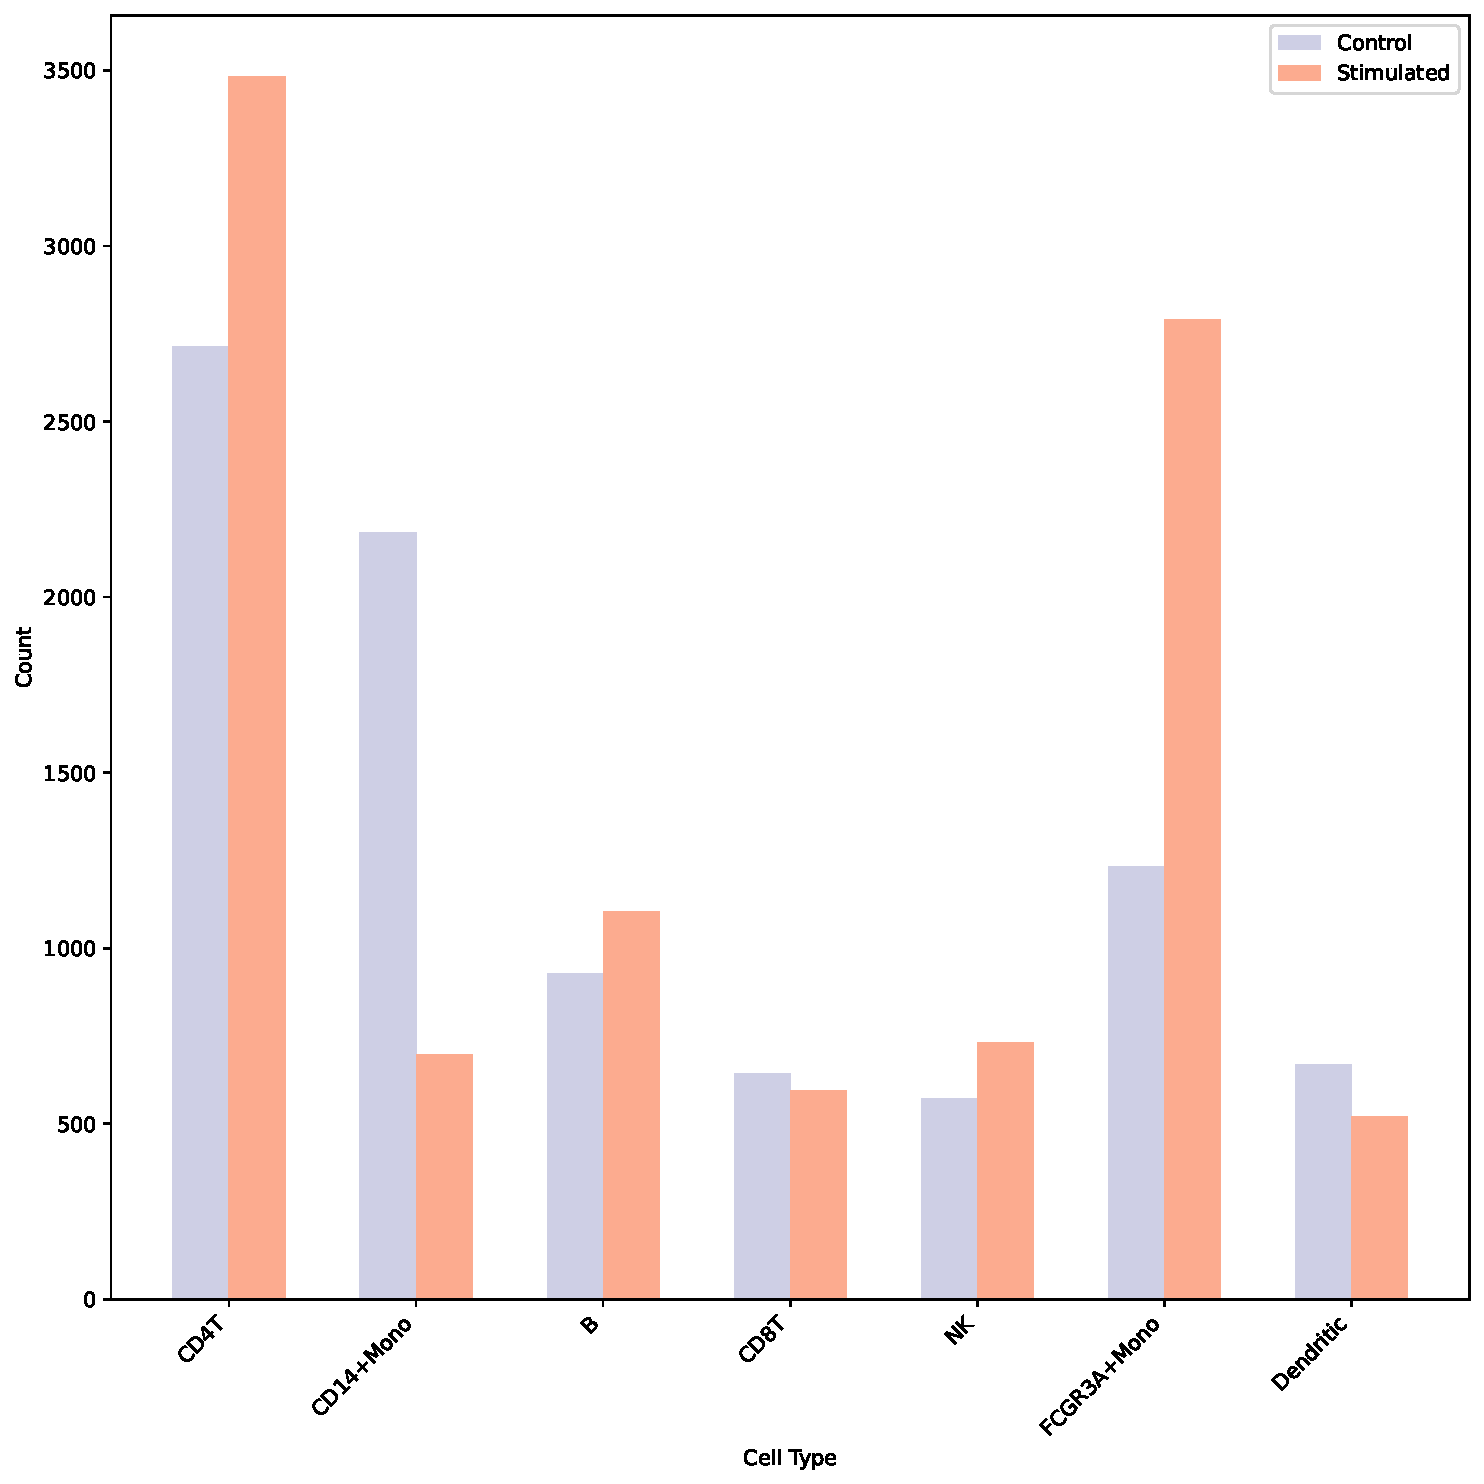
\includegraphics[width=.9\textwidth]{figures/pbmc_counts.pdf}
        \caption{}
        \label{fig:figure3}
    \end{subfigure}
    \caption{PBMC overview}
    \label{fig:combined}
\end{figure}

\clearpage

\begin{figure}
    \centering
    \begin{minipage}{0.4\textwidth}
        \centering
        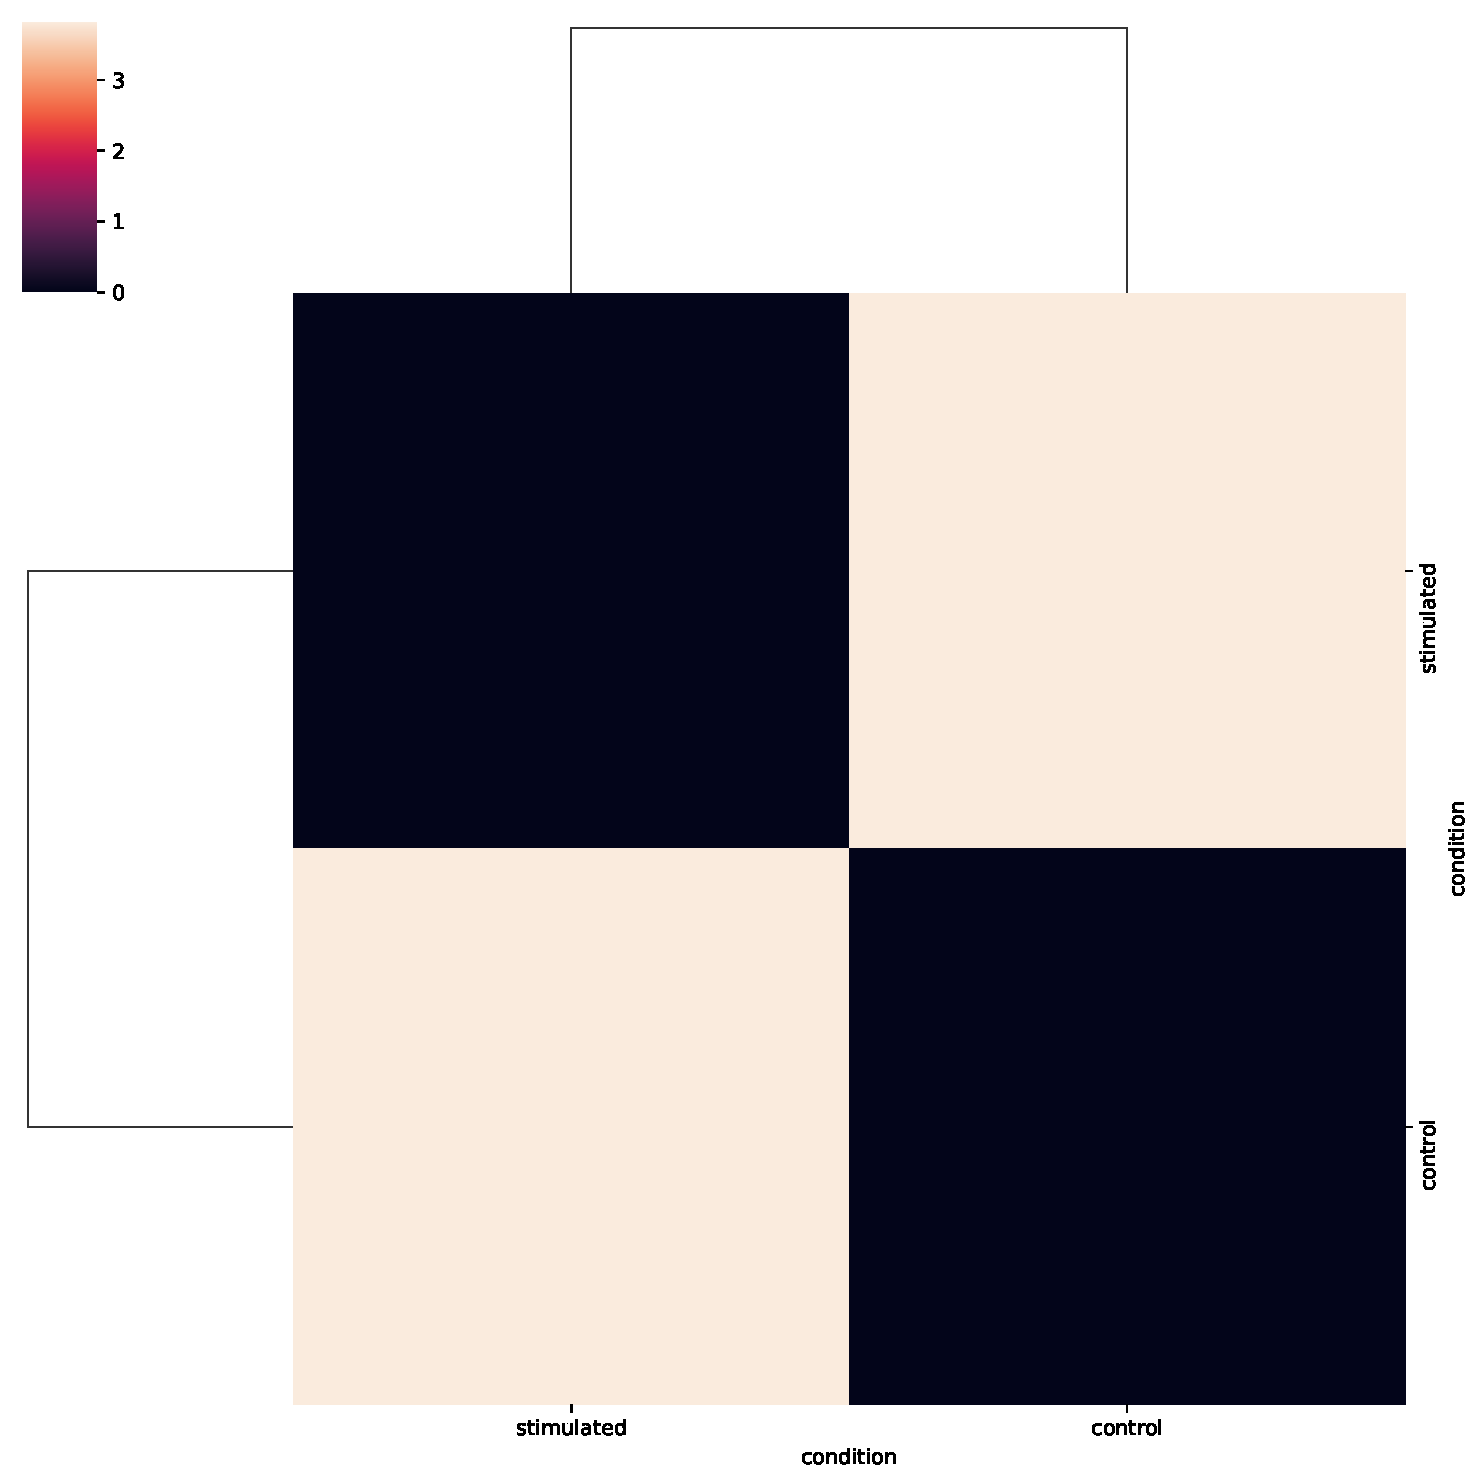
\includegraphics[width=\textwidth]{figures/pbmc_condition_edistance_clustermap.pdf}
        \caption{E-distance}
    \end{minipage} \hfill
    \begin{minipage}{0.4\textwidth}
        \centering
        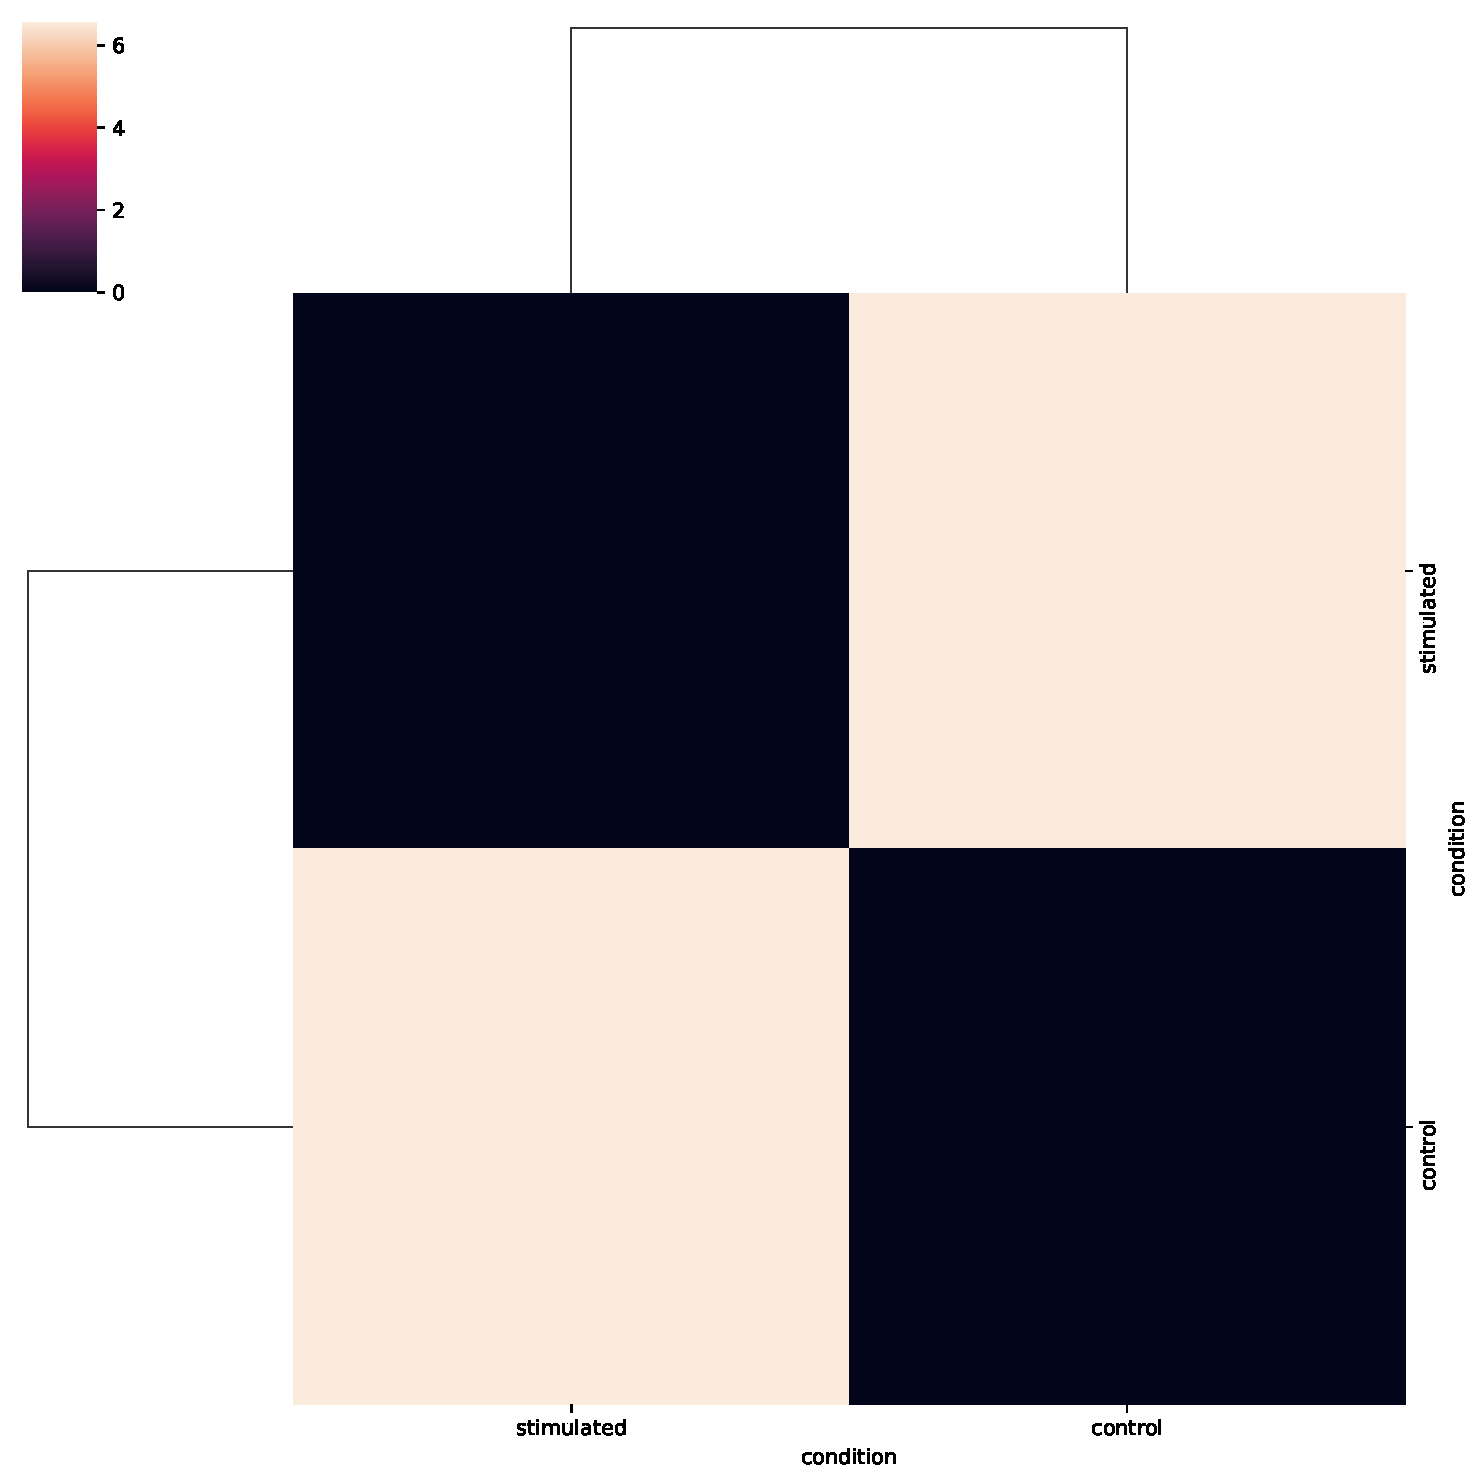
\includegraphics[width=\textwidth]{figures/pbmc_condition_euclidean_clustermap.pdf}
        \caption{Euclidean}
    \end{minipage}
    \vskip\baselineskip

    \begin{minipage}{0.4\textwidth}
        \centering
        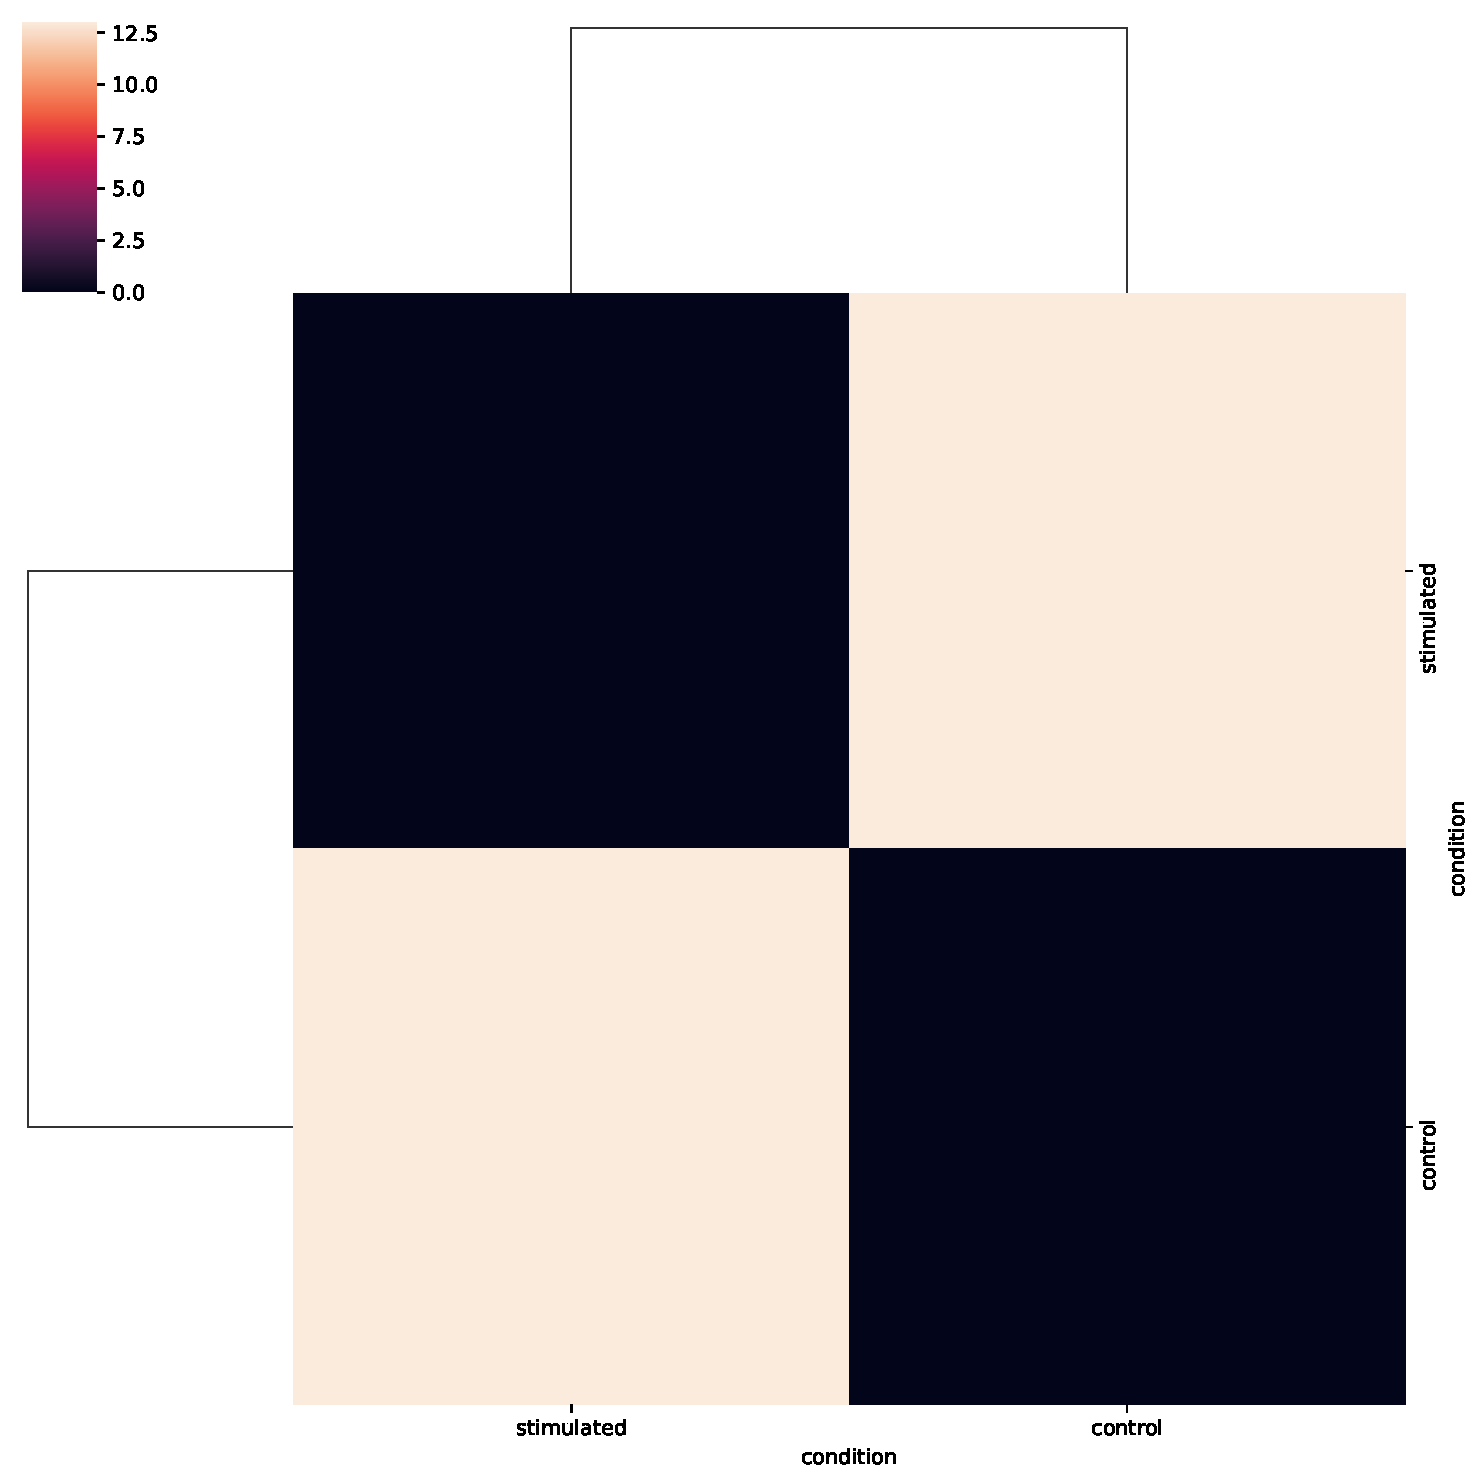
\includegraphics[width=\textwidth]{figures/pbmc_condition_mean_pairwise_clustermap.pdf}
        \caption{Mean pairwise}
    \end{minipage} \hfill
    \begin{minipage}{0.4\textwidth}
        \centering
        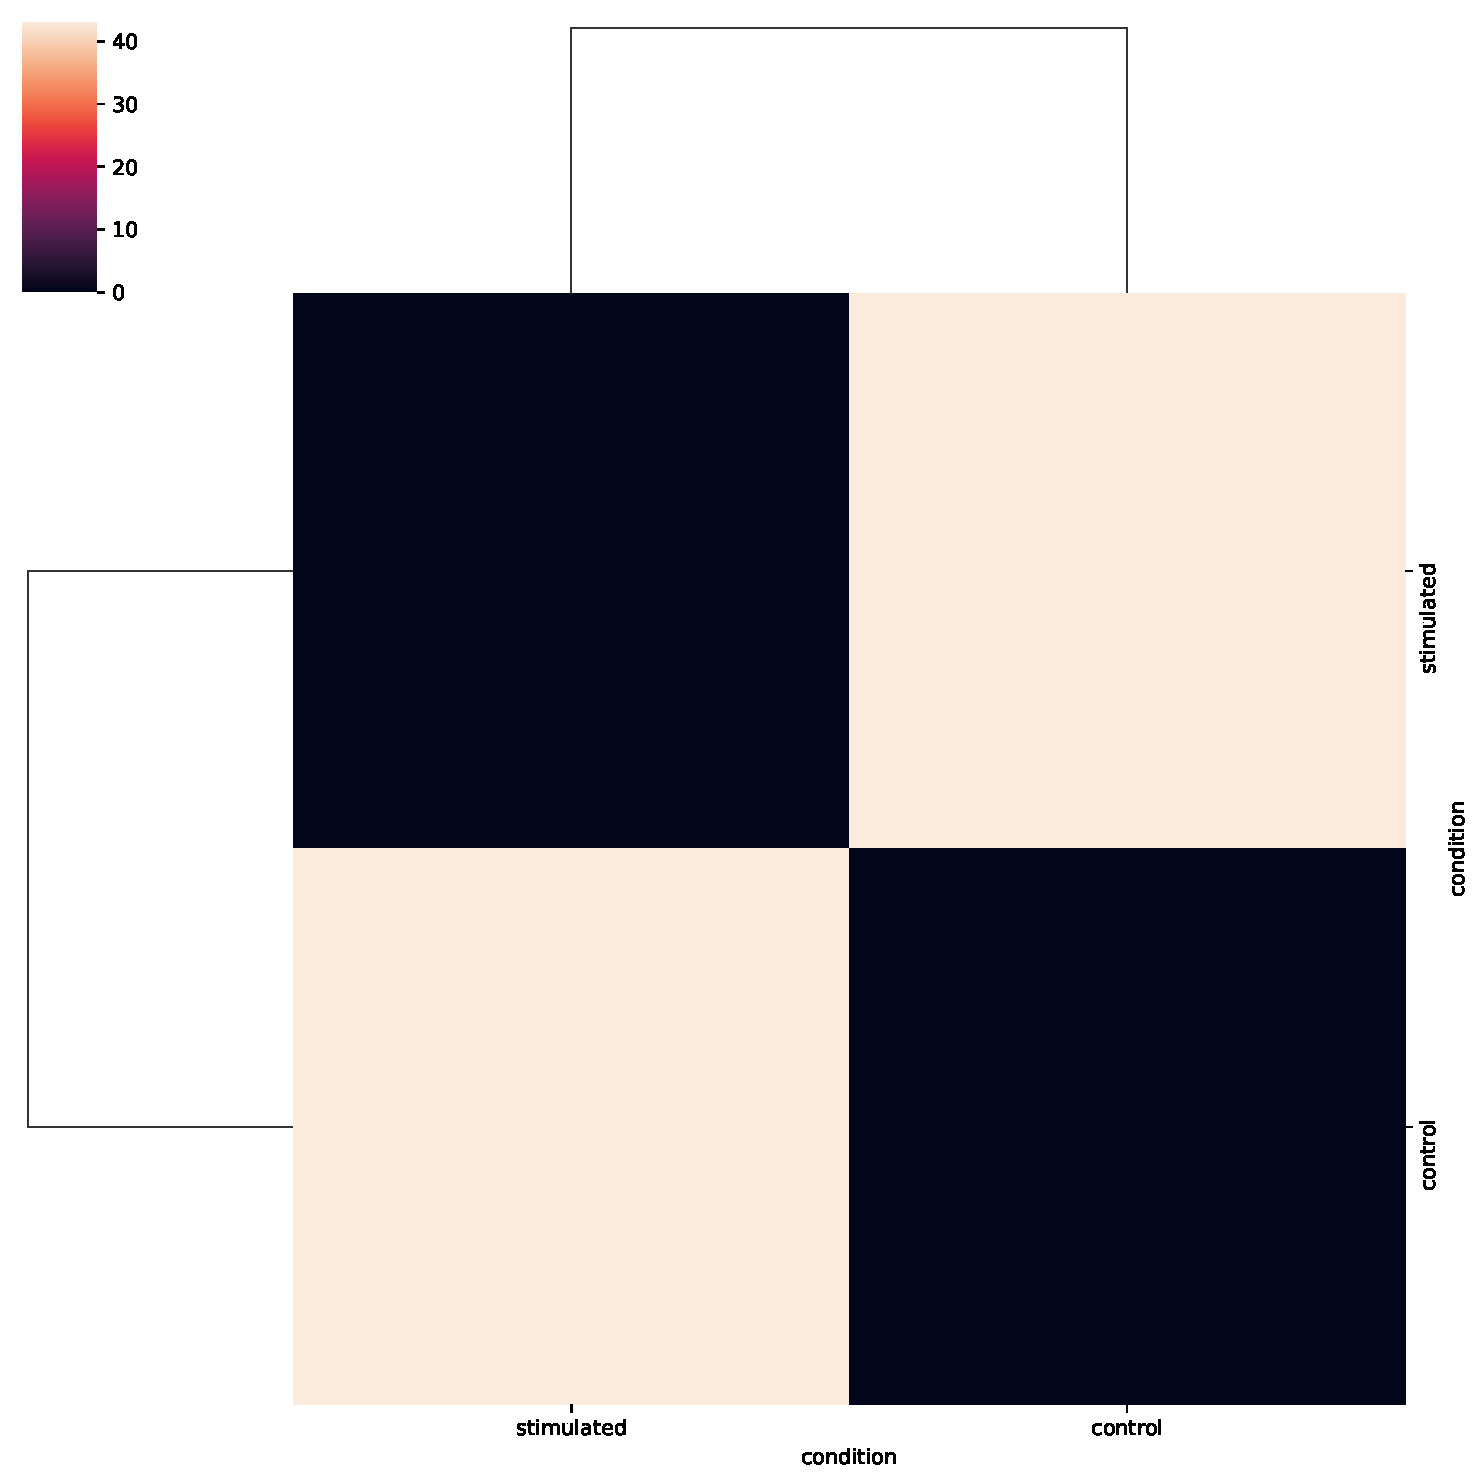
\includegraphics[width=\textwidth]{figures/pbmc_condition_mmd_clustermap.pdf}
        \caption{MMD}
    \end{minipage}
    \vskip\baselineskip

    \begin{minipage}{0.4\textwidth}
        \centering
        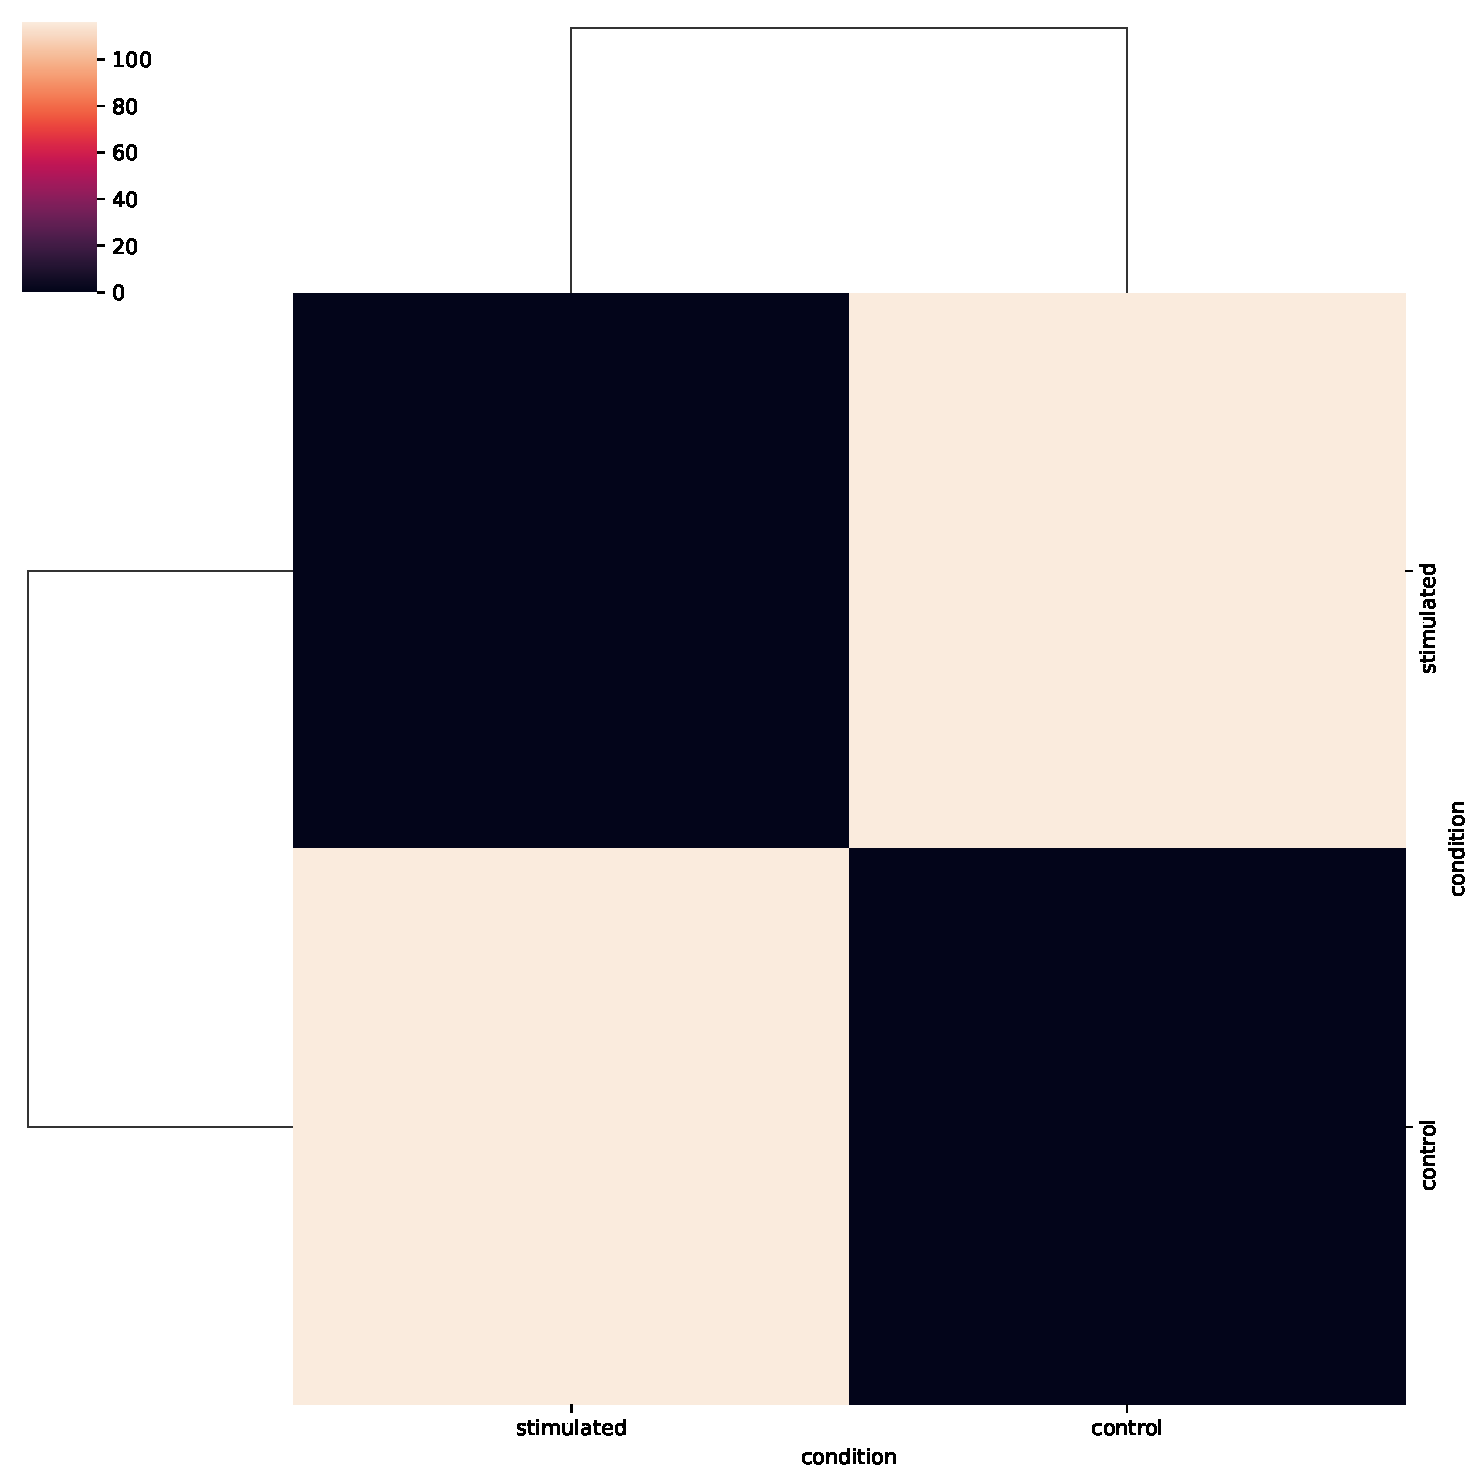
\includegraphics[width=\textwidth]{figures/pbmc_condition_wasserstein_clustermap.pdf}
        \caption{Wasserstein}
    \end{minipage}
    \caption{Distance metrics per condition}
\end{figure}

\clearpage


\begin{figure}
    \centering
    \begin{minipage}{0.4\textwidth}
        \centering
        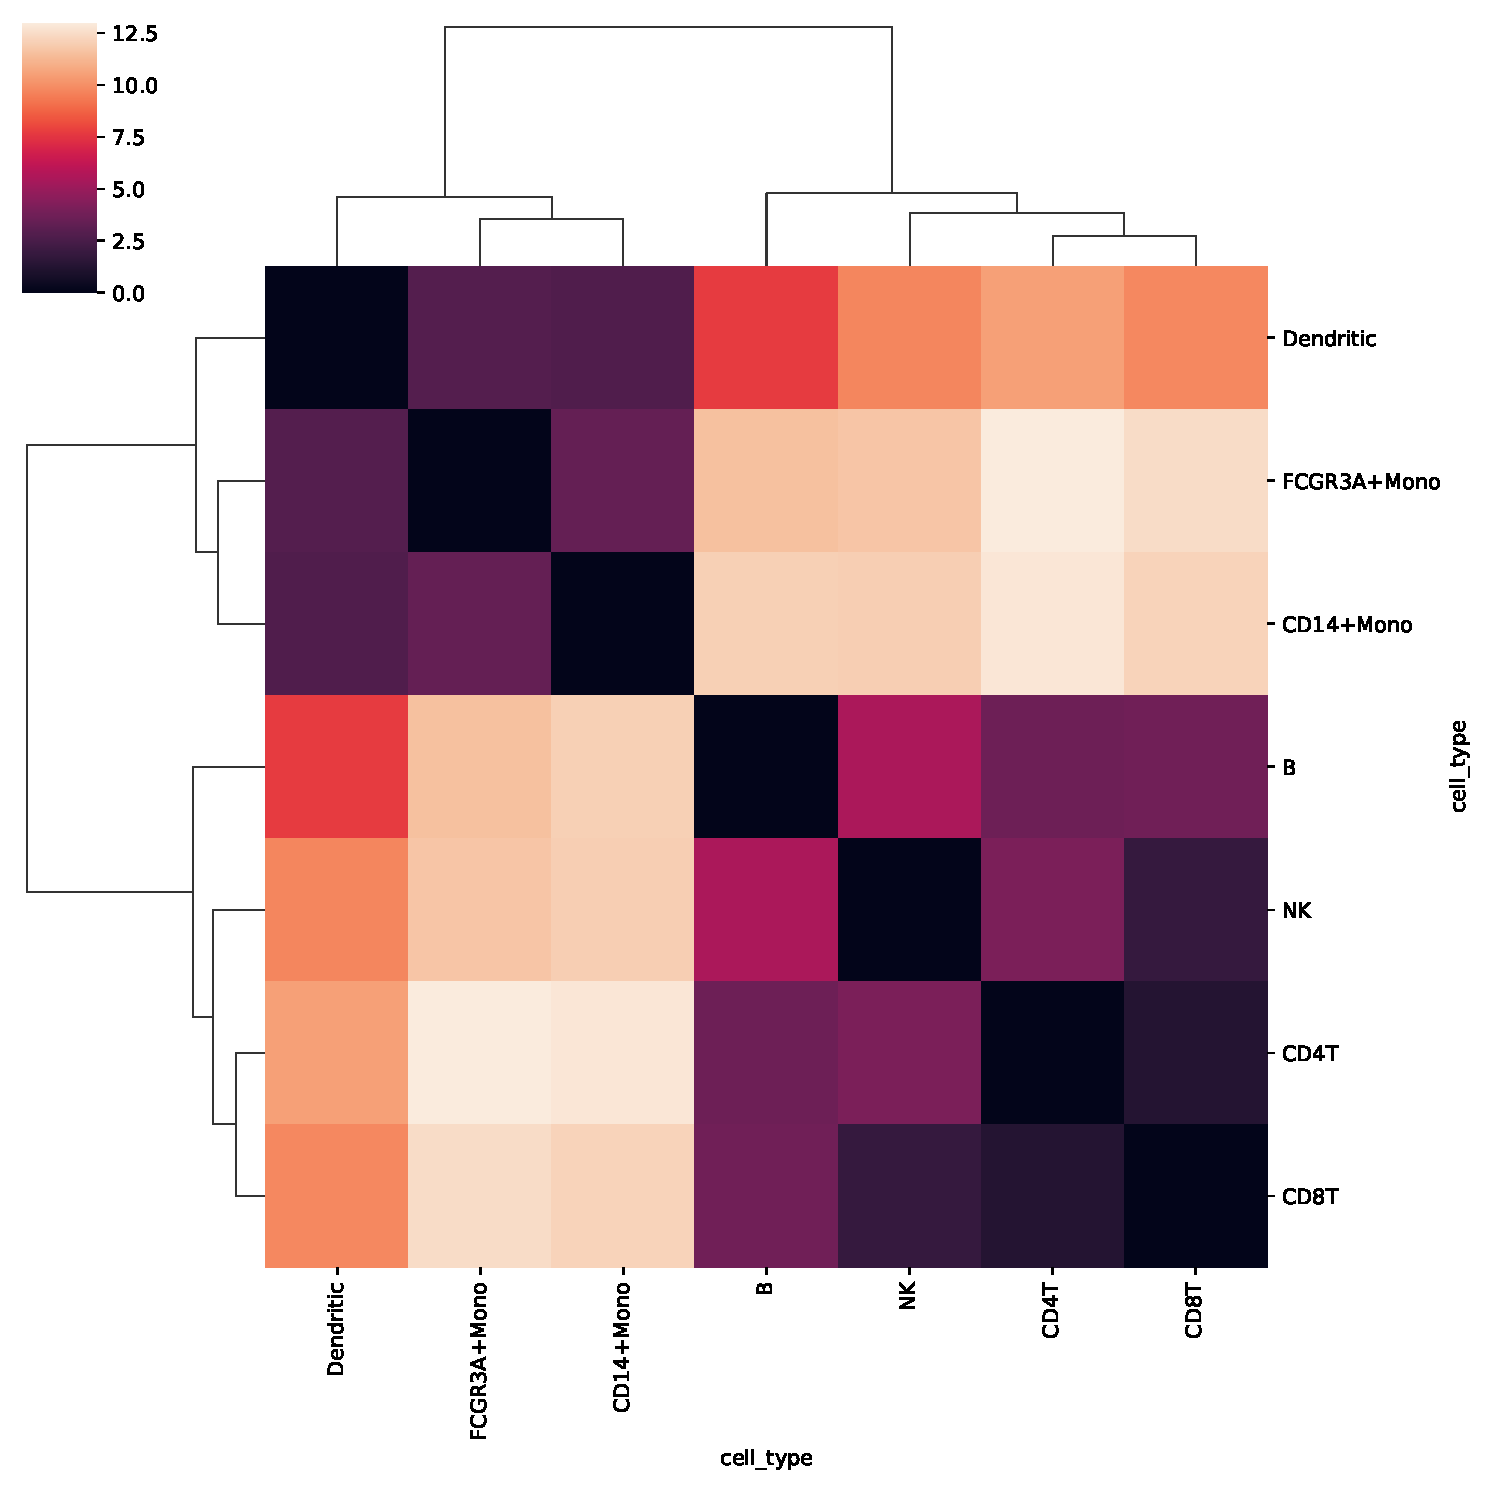
\includegraphics[width=\textwidth]{figures/pbmc_cell_type_edistance_clustermap.pdf}
        \caption{E-distance}
    \end{minipage} \hfill
    \begin{minipage}{0.4\textwidth}
        \centering
        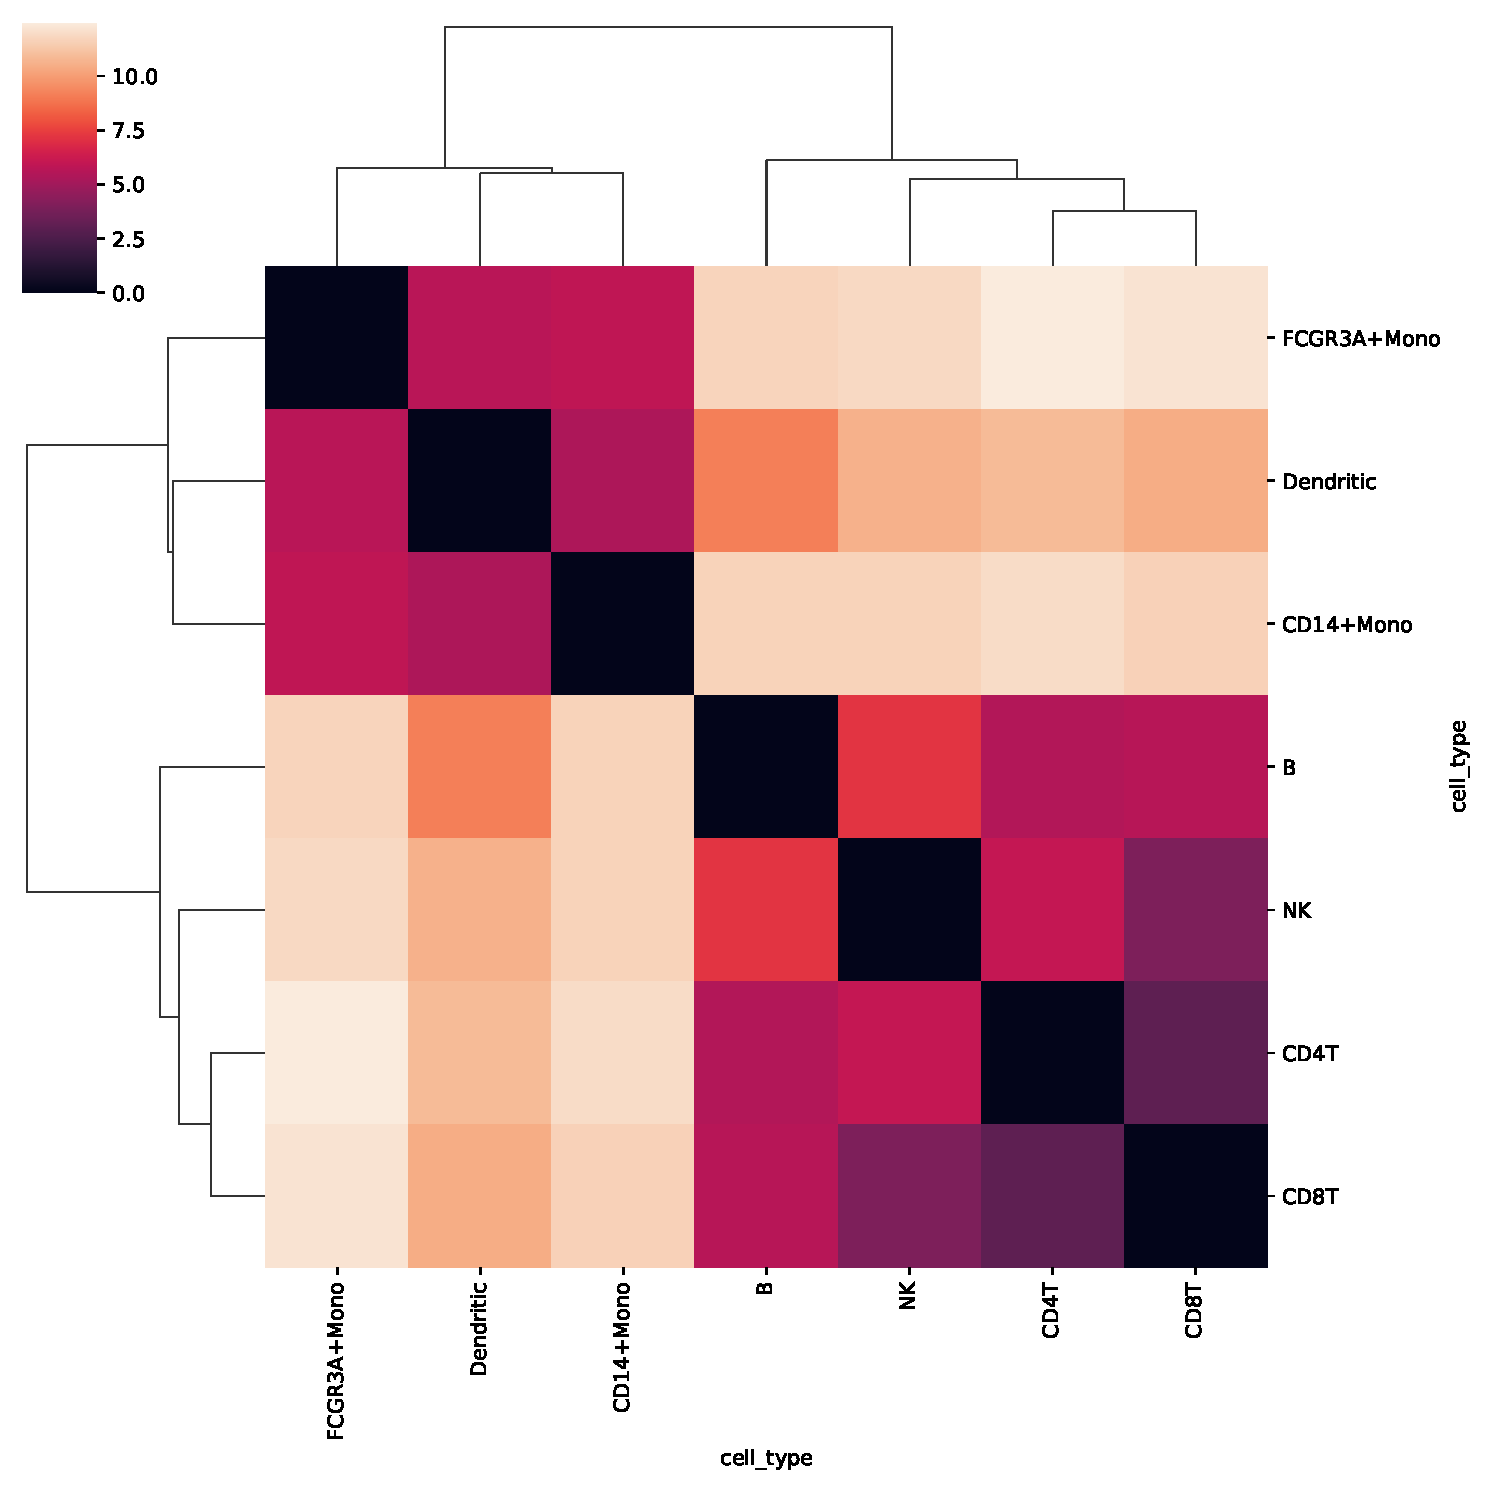
\includegraphics[width=\textwidth]{figures/pbmc_cell_type_euclidean_clustermap.pdf}
        \caption{Euclidean}
    \end{minipage}
    \vskip\baselineskip

    \begin{minipage}{0.4\textwidth}
        \centering
        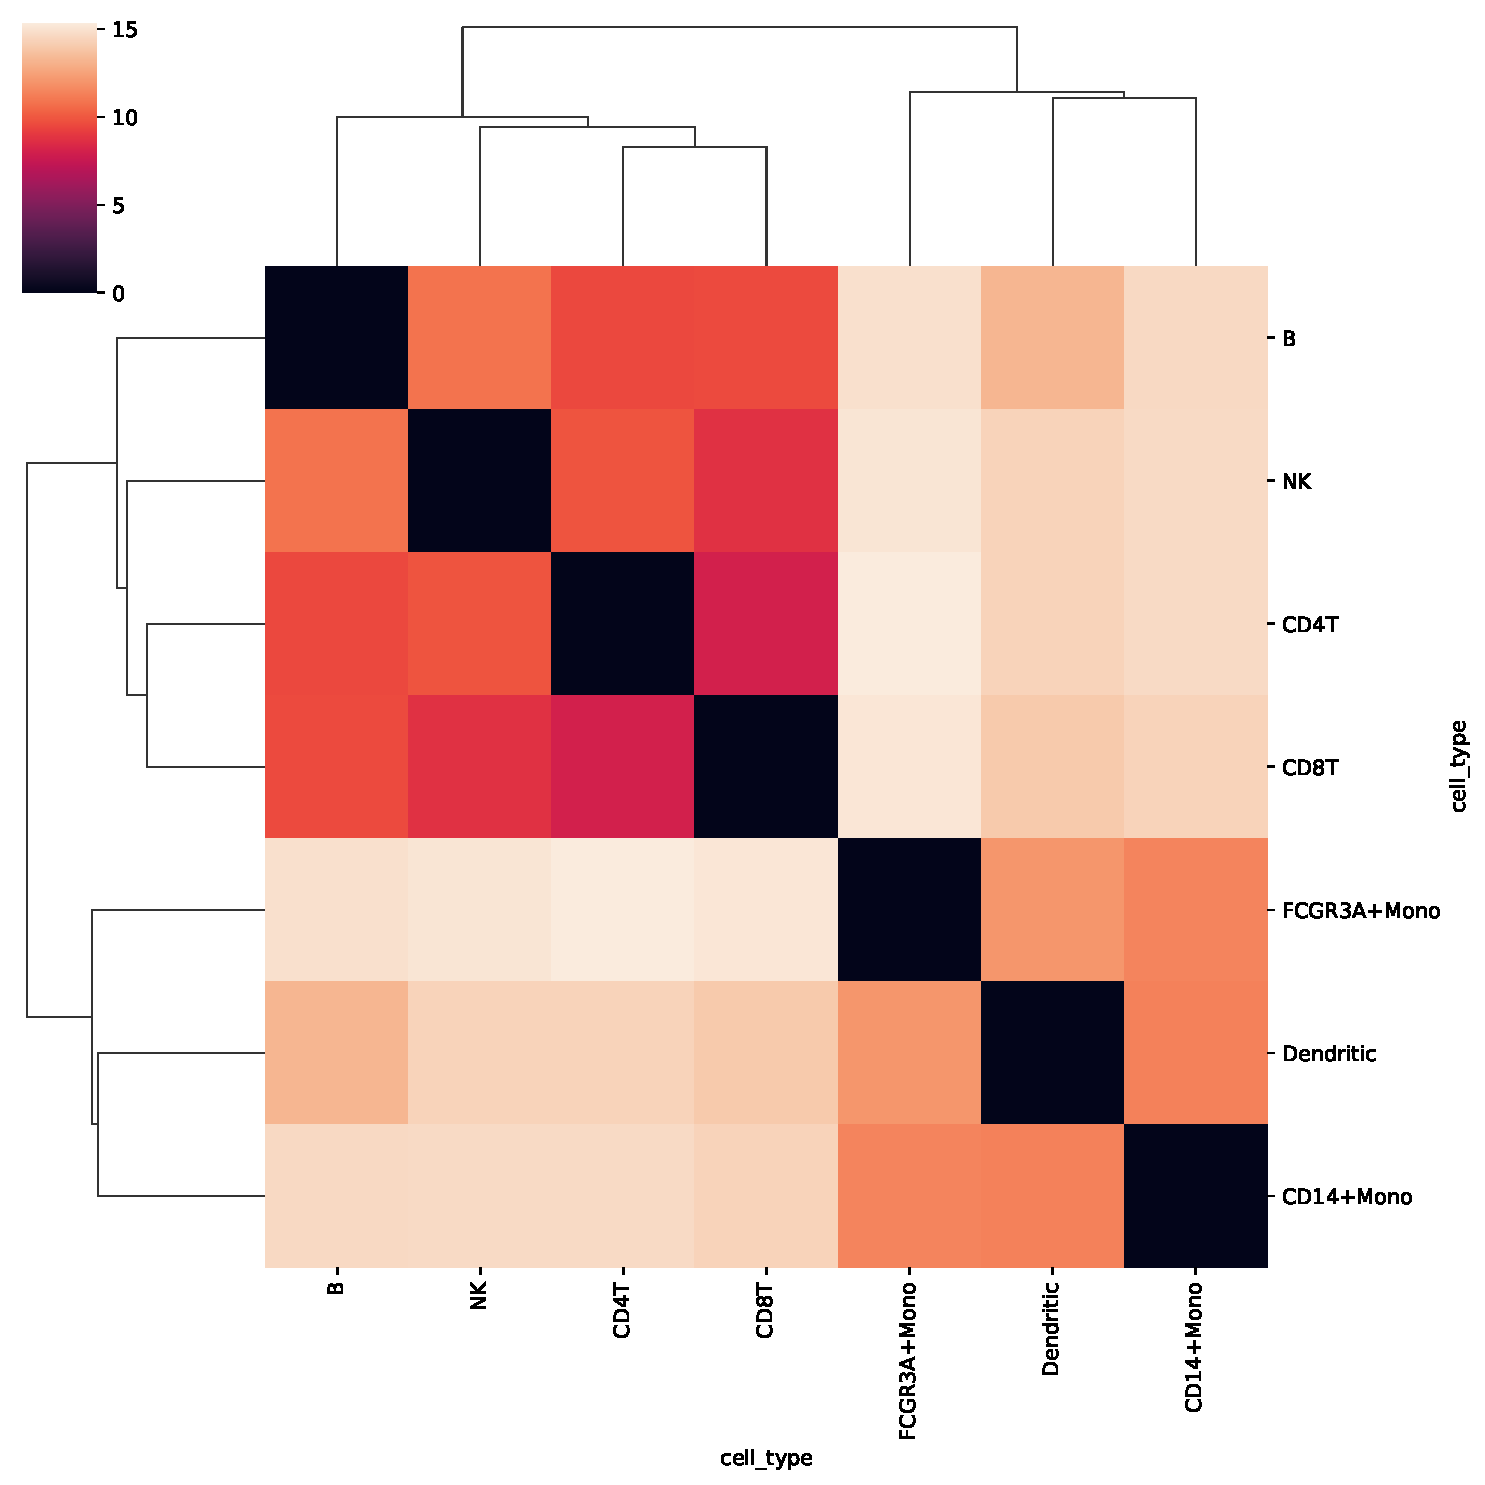
\includegraphics[width=\textwidth]{figures/pbmc_cell_type_mean_pairwise_clustermap.pdf}
        \caption{Mean pairwise}
    \end{minipage} \hfill
    \begin{minipage}{0.4\textwidth}
        \centering
        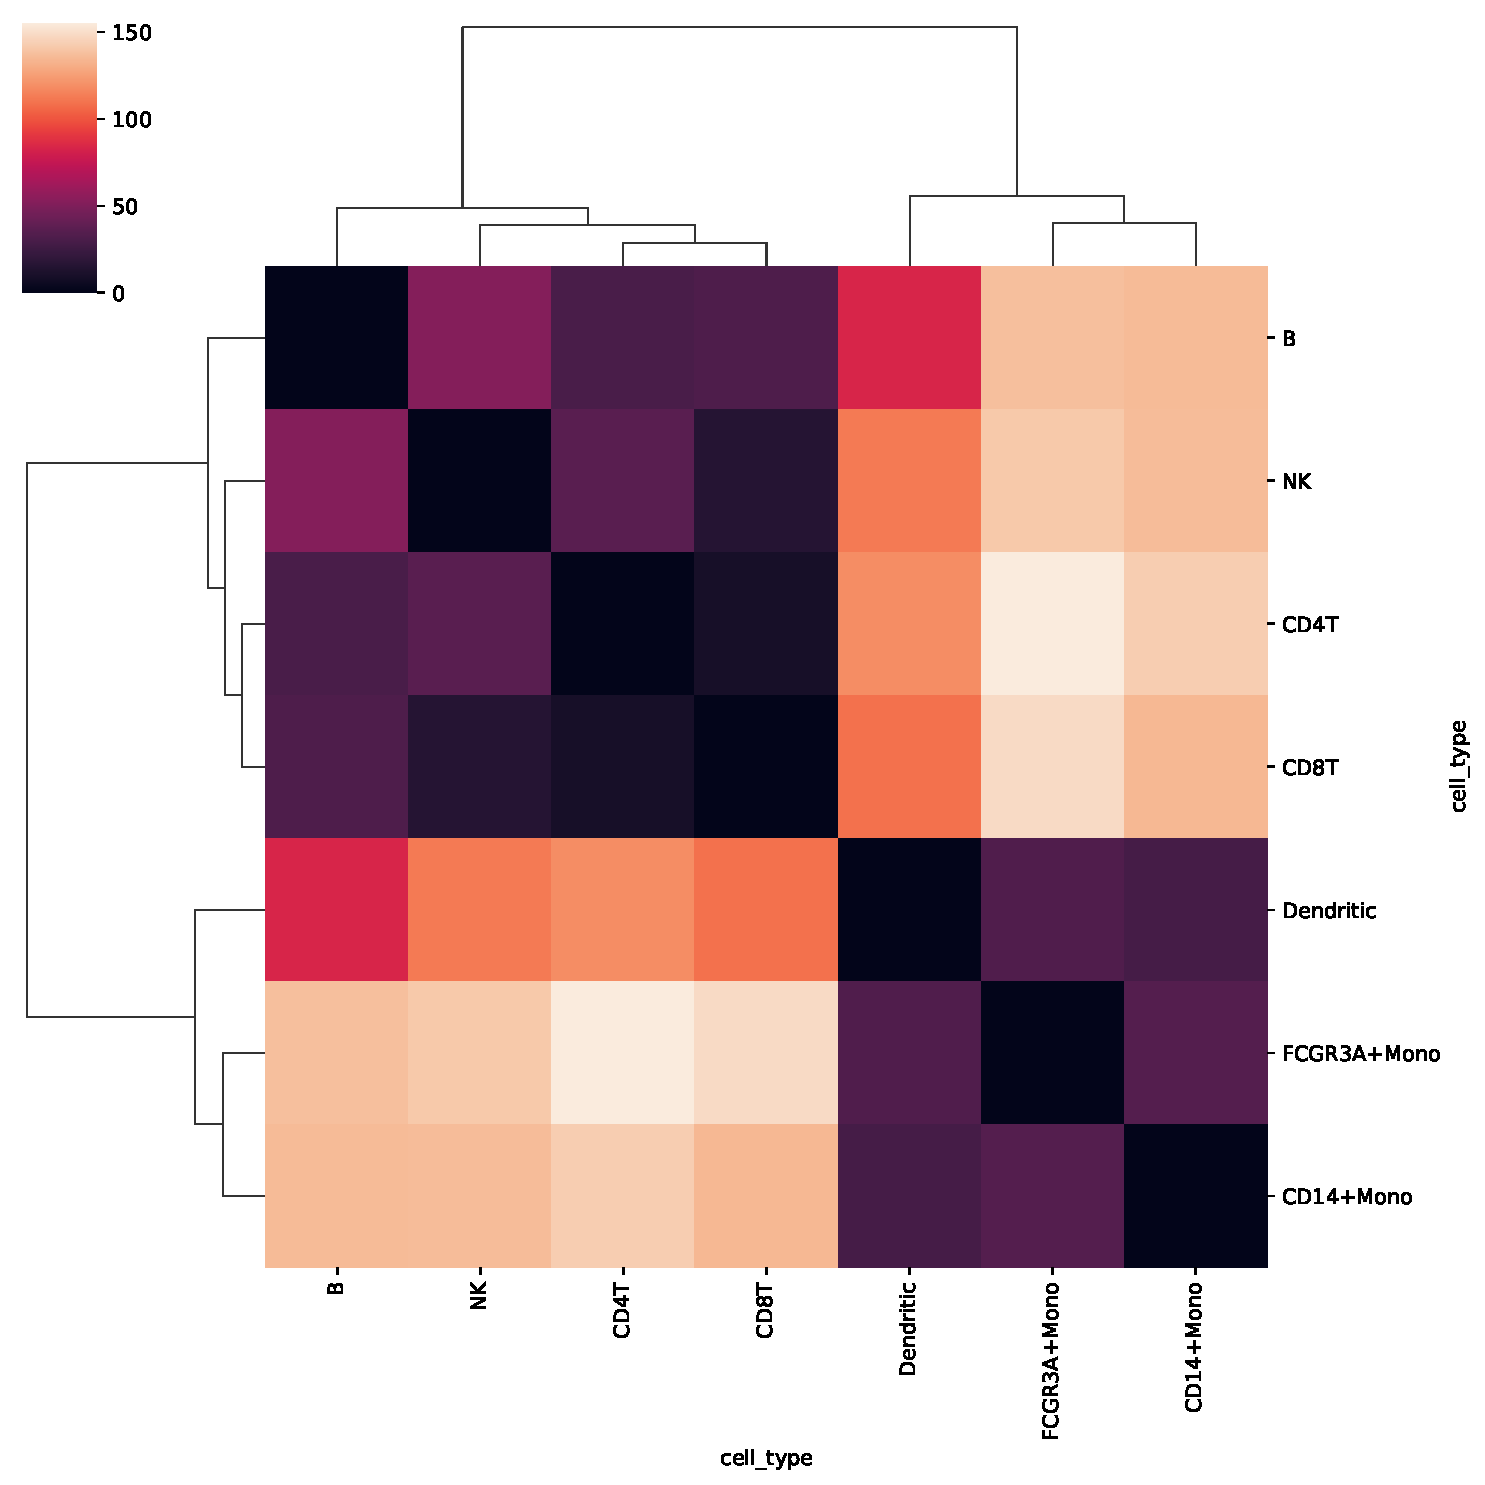
\includegraphics[width=\textwidth]{figures/pbmc_cell_type_mmd_clustermap.pdf}
        \caption{MMD}
    \end{minipage}
    \vskip\baselineskip

    \begin{minipage}{0.4\textwidth}
        \centering
        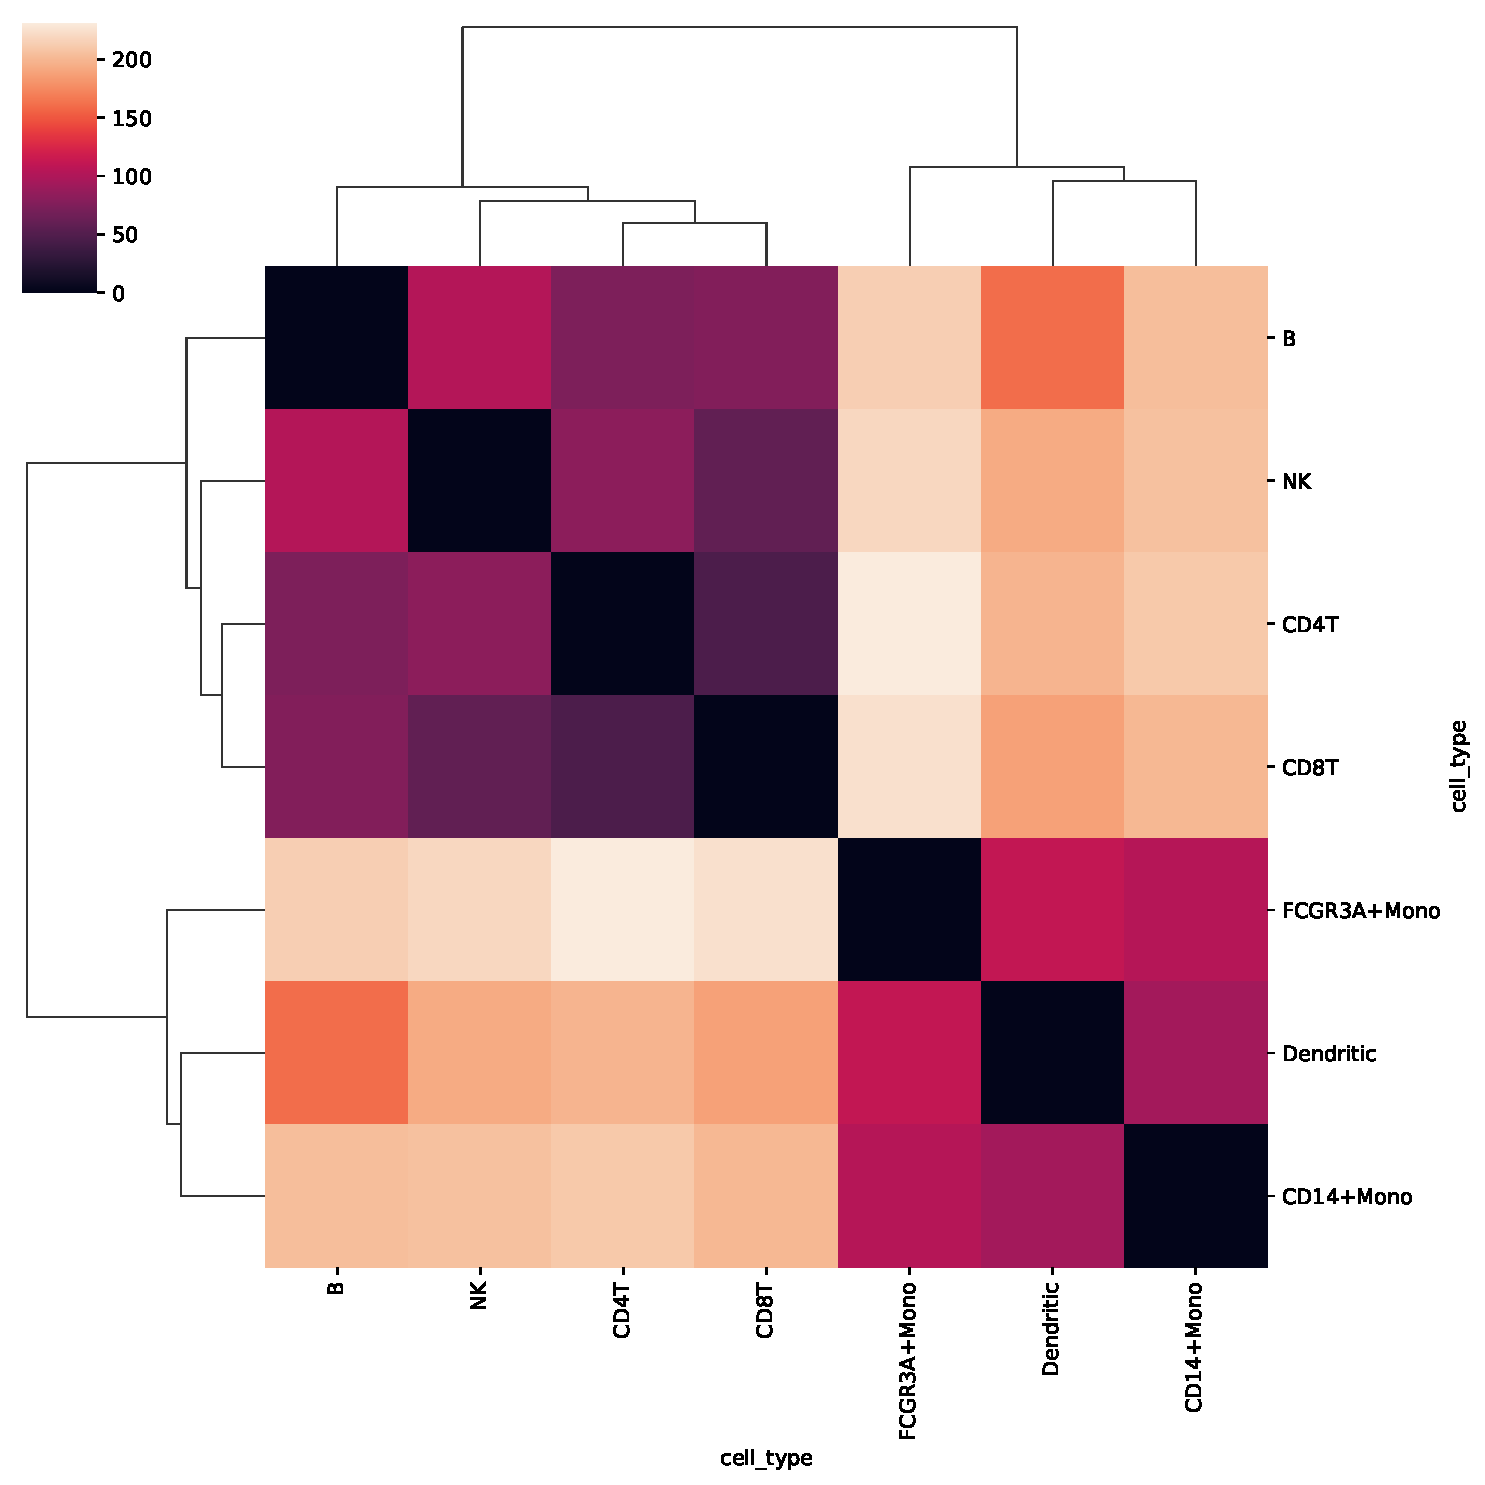
\includegraphics[width=\textwidth]{figures/pbmc_cell_type_wasserstein_clustermap.pdf}
        \caption{Wasserstein}
    \end{minipage}
    \caption{Distance metrics per cell type}
\end{figure}

\clearpage


\section{Nault all cell types evaluation}

\subsection{Multiple doses}

\begin{figure}[h!]
    \centering
    \includegraphics[width=.8\textwidth]{figures/nault_umap_split_multiple.png}
\end{figure}

\begin{figure}[h!]
    \centering
    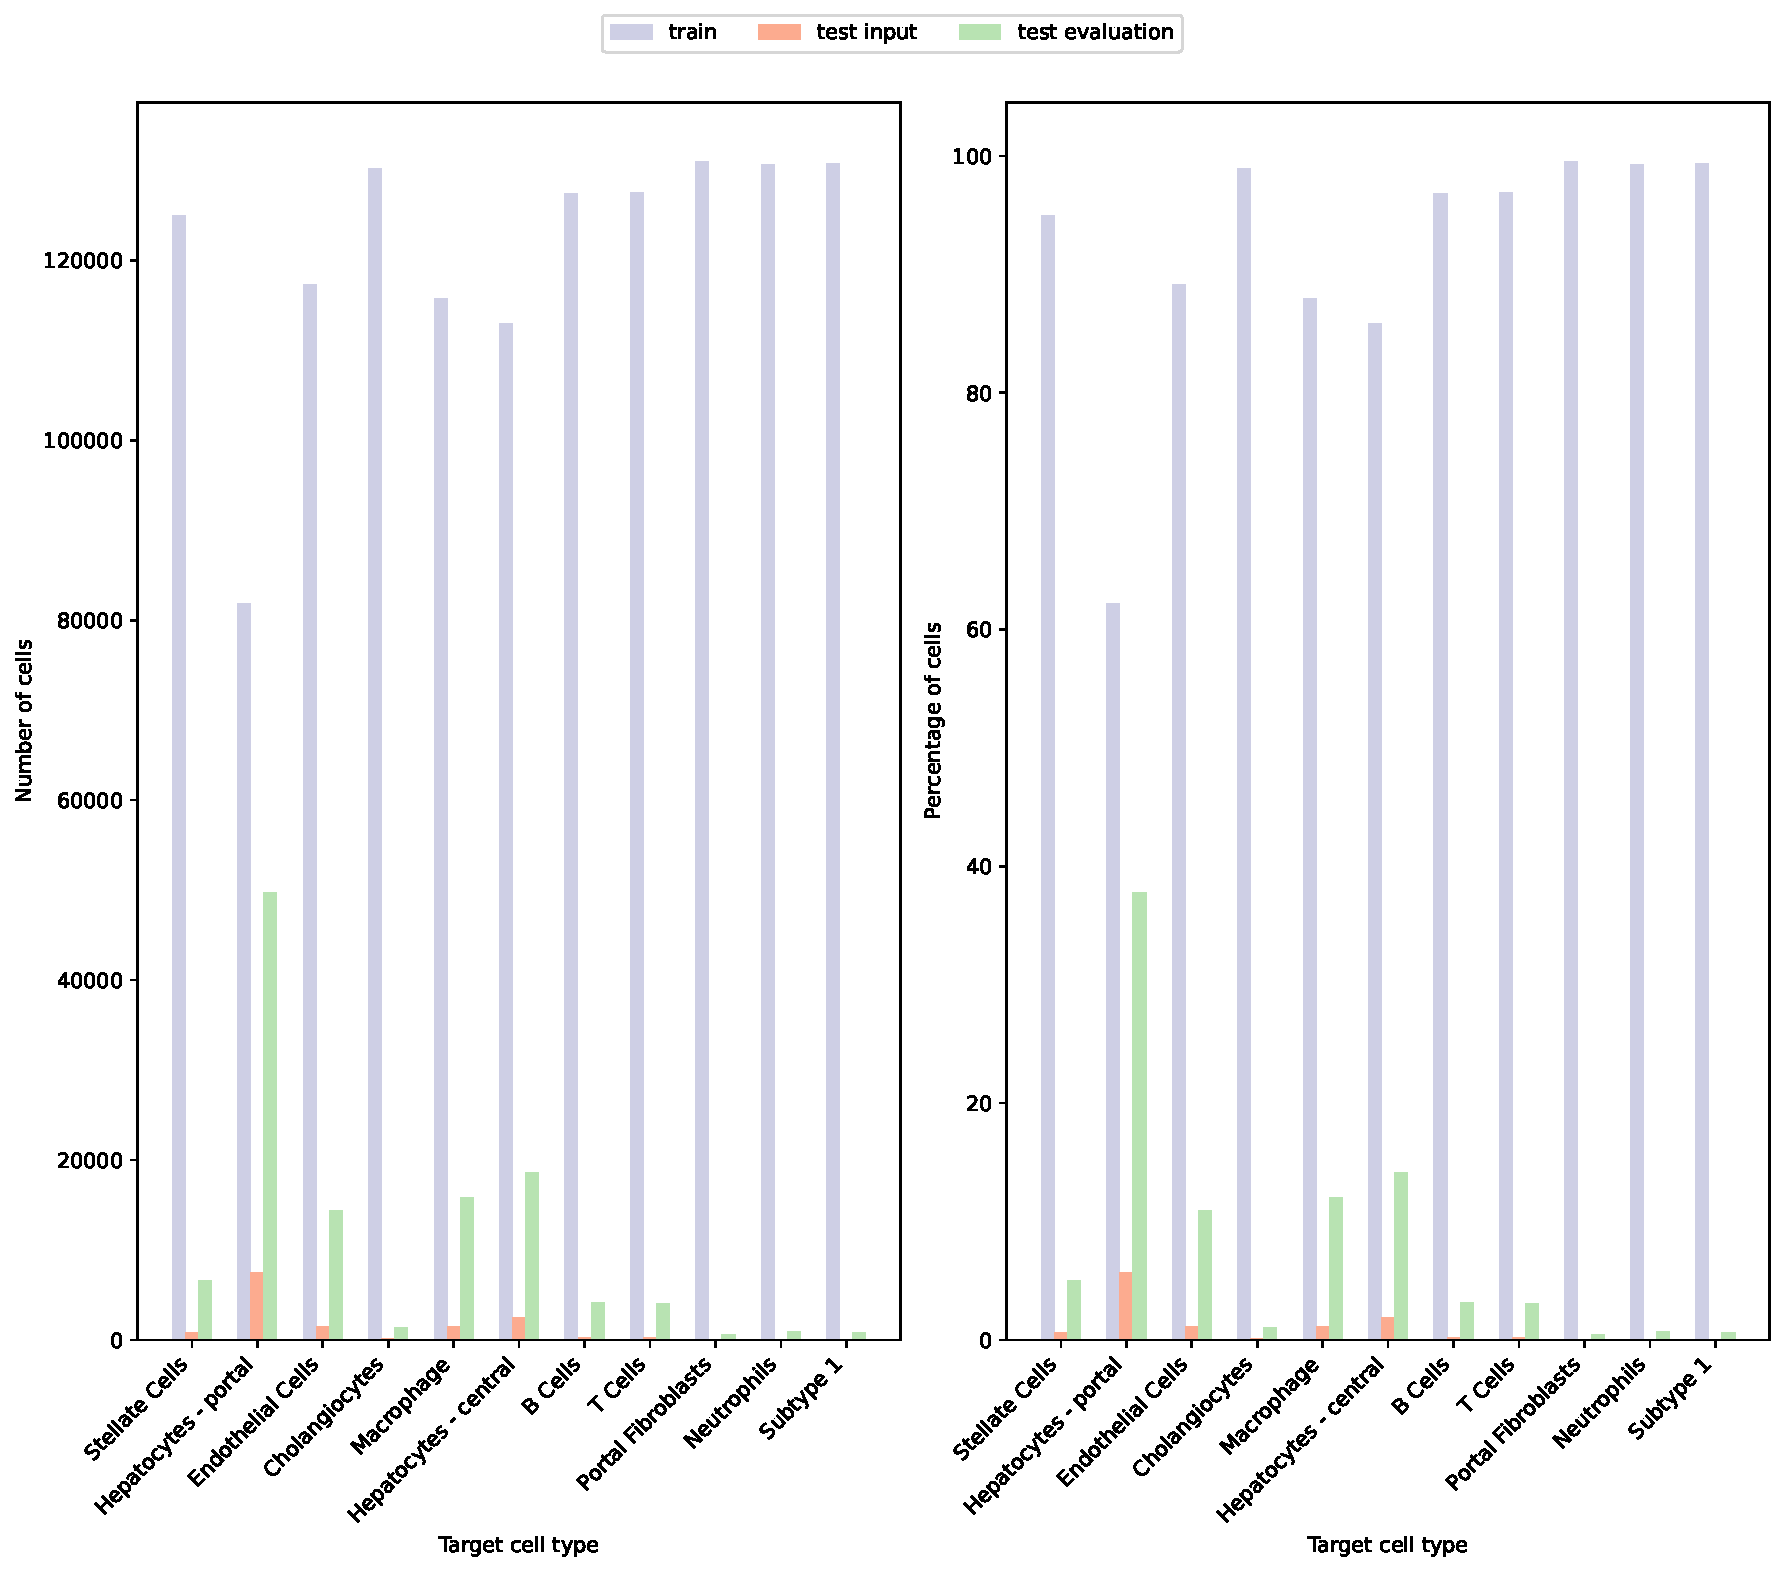
\includegraphics[width=.8\textwidth]{figures/nault_bars_split_multiple.pdf}
\end{figure}


\subsection{Single dose}


\begin{figure}[h!]
    \centering
    \includegraphics[width=.7\textwidth]{figures/nault_umap_split_30.png}
    \caption{Example of $30 \mu g/kg$}
\end{figure}

\begin{figure}[h!]
    \centering
    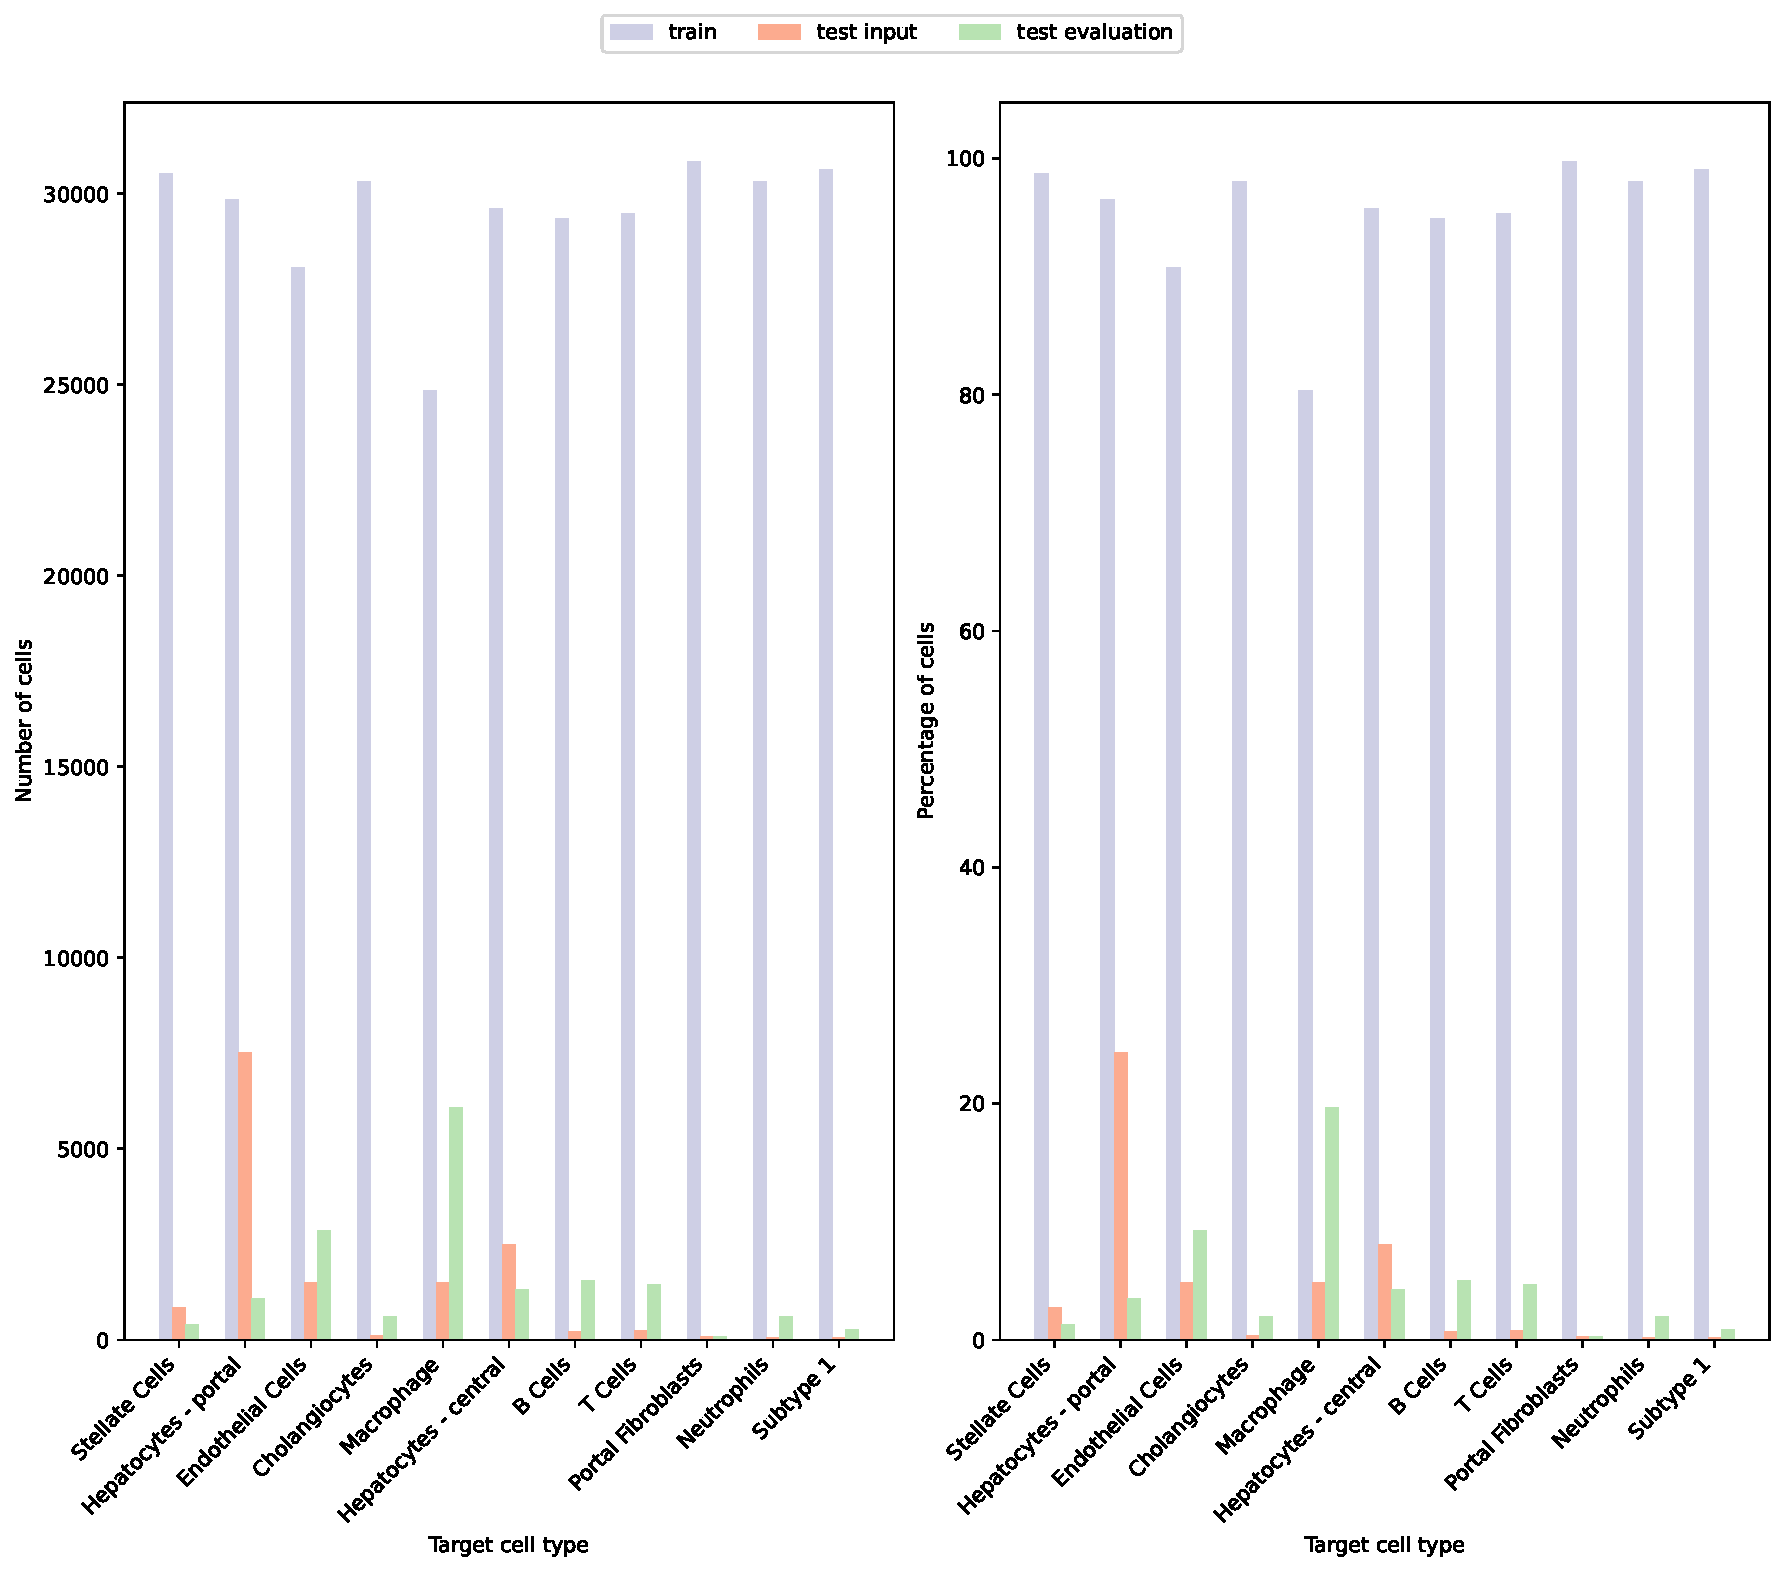
\includegraphics[width=.7\textwidth]{figures/nault_bars_split_30.pdf}
    \caption{Number of cells per cell type for $30 \mu g/kg$}
\end{figure}

\clearpage


\subsection{Comparison}


\begin{figure}[h!]
    \centering
    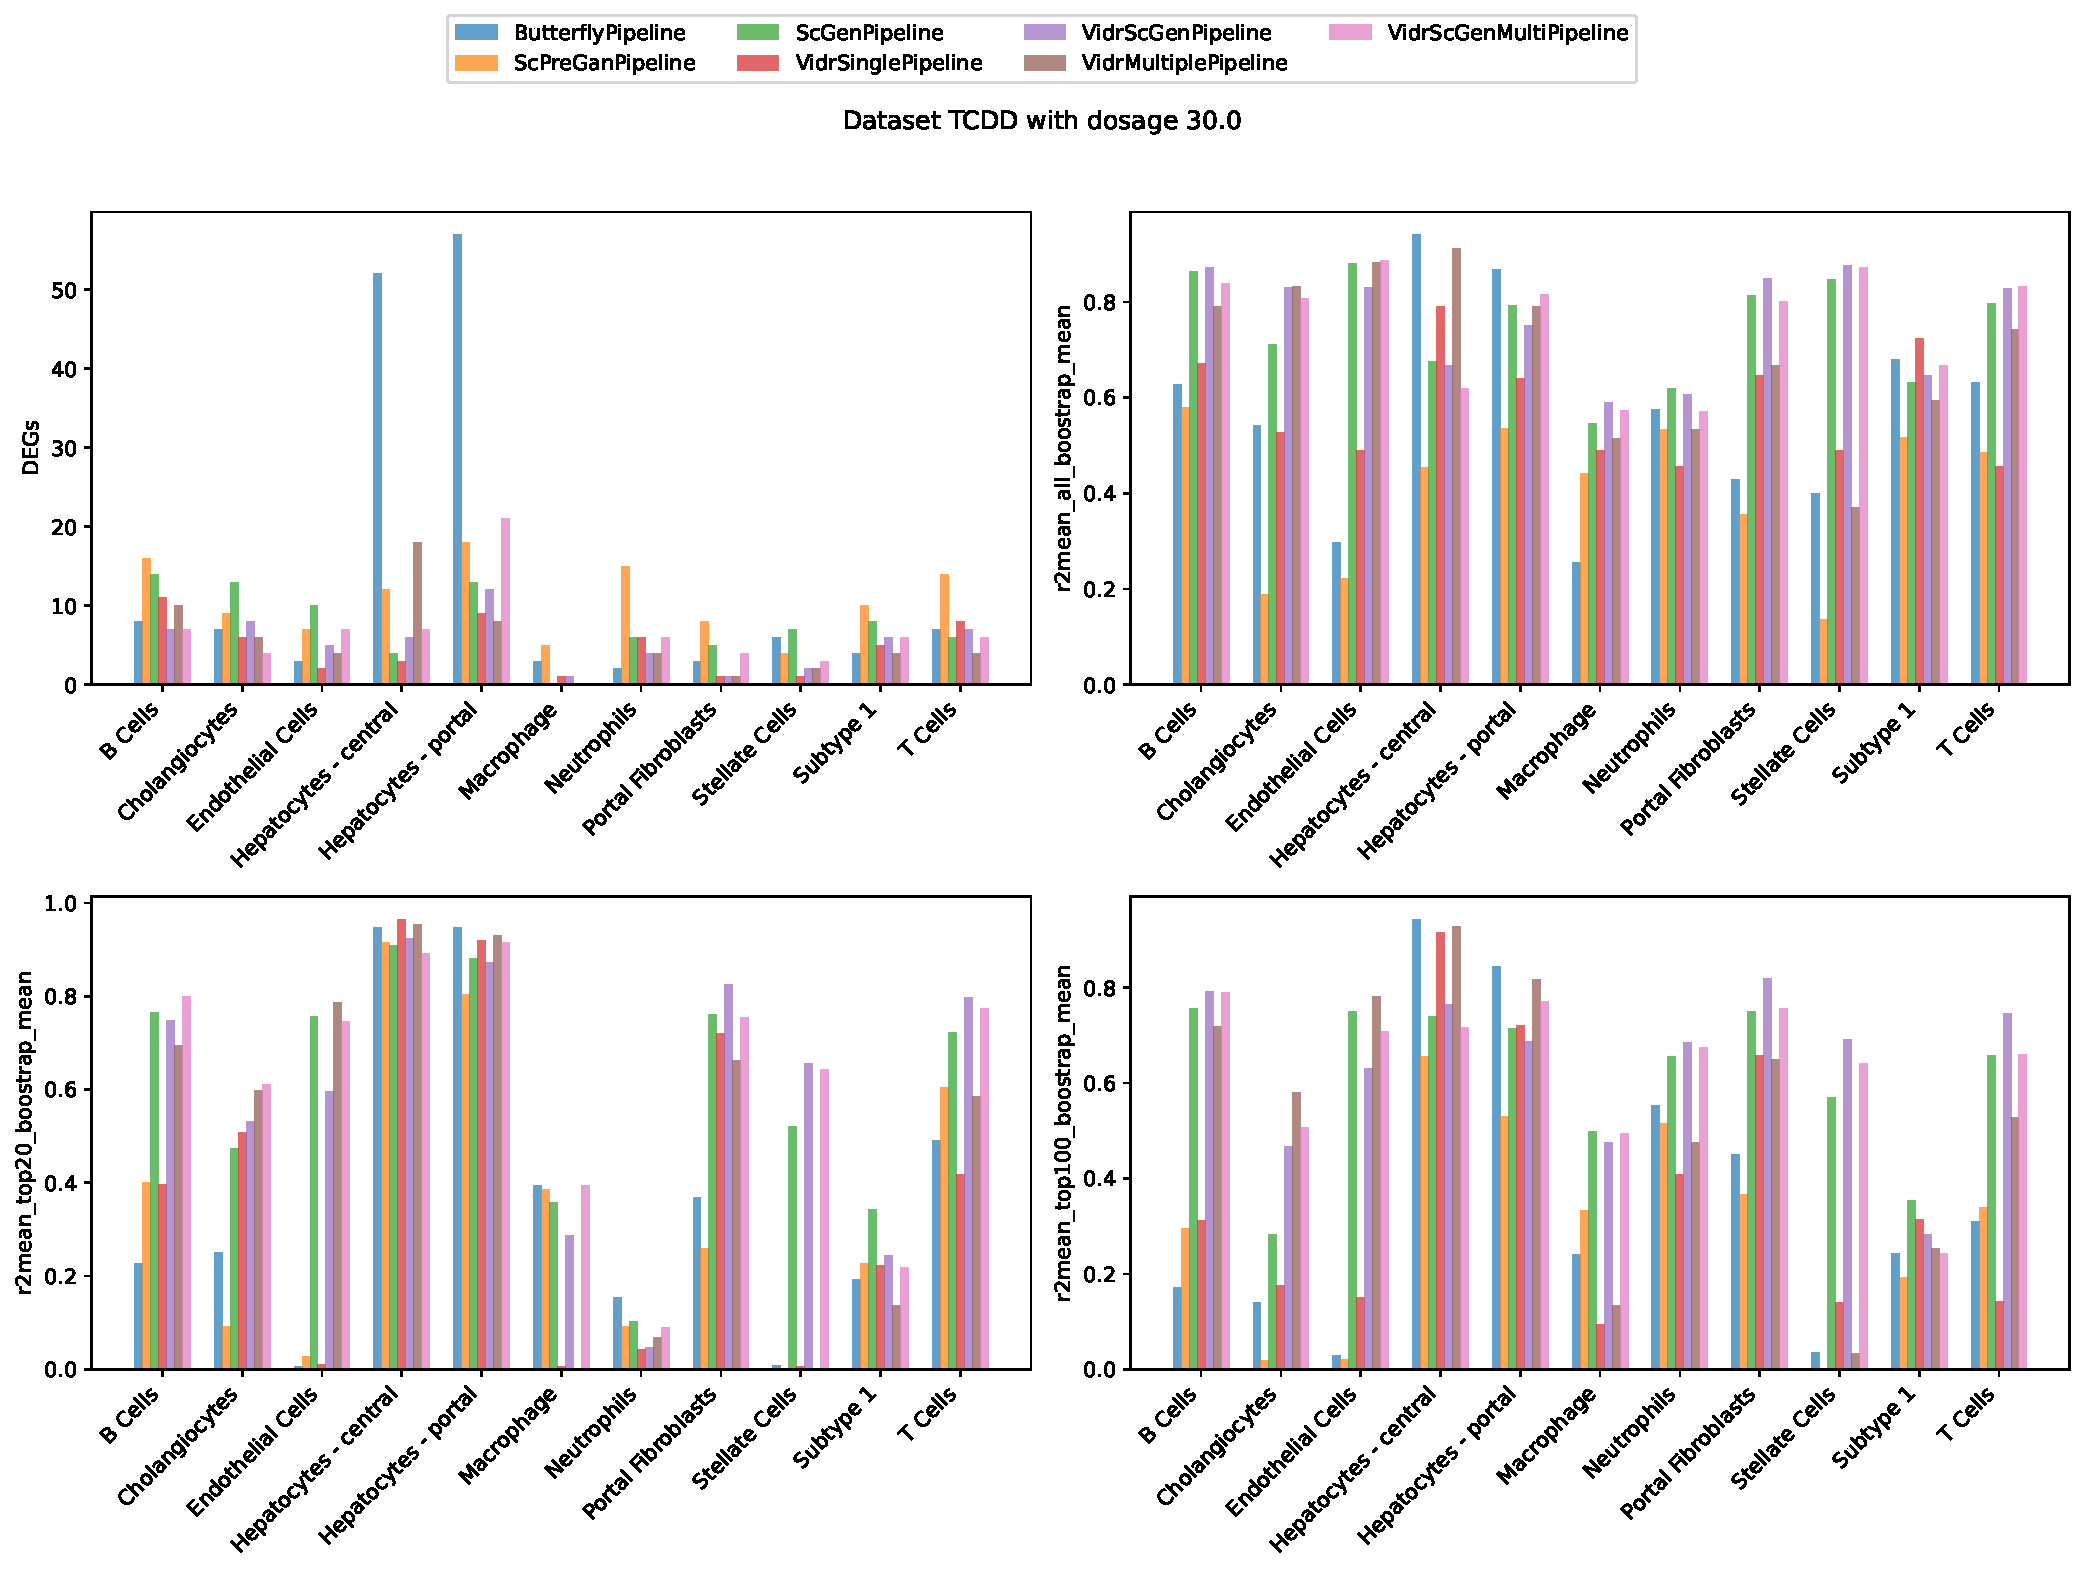
\includegraphics[width=.8\textwidth]{figures/nault_30_baseline_metrics_bars.pdf}
    \caption{Baseline metrics for highest dosage $30 \mu g/kg$ across cell types}
\end{figure}

\begin{figure}[h!]
    \centering
    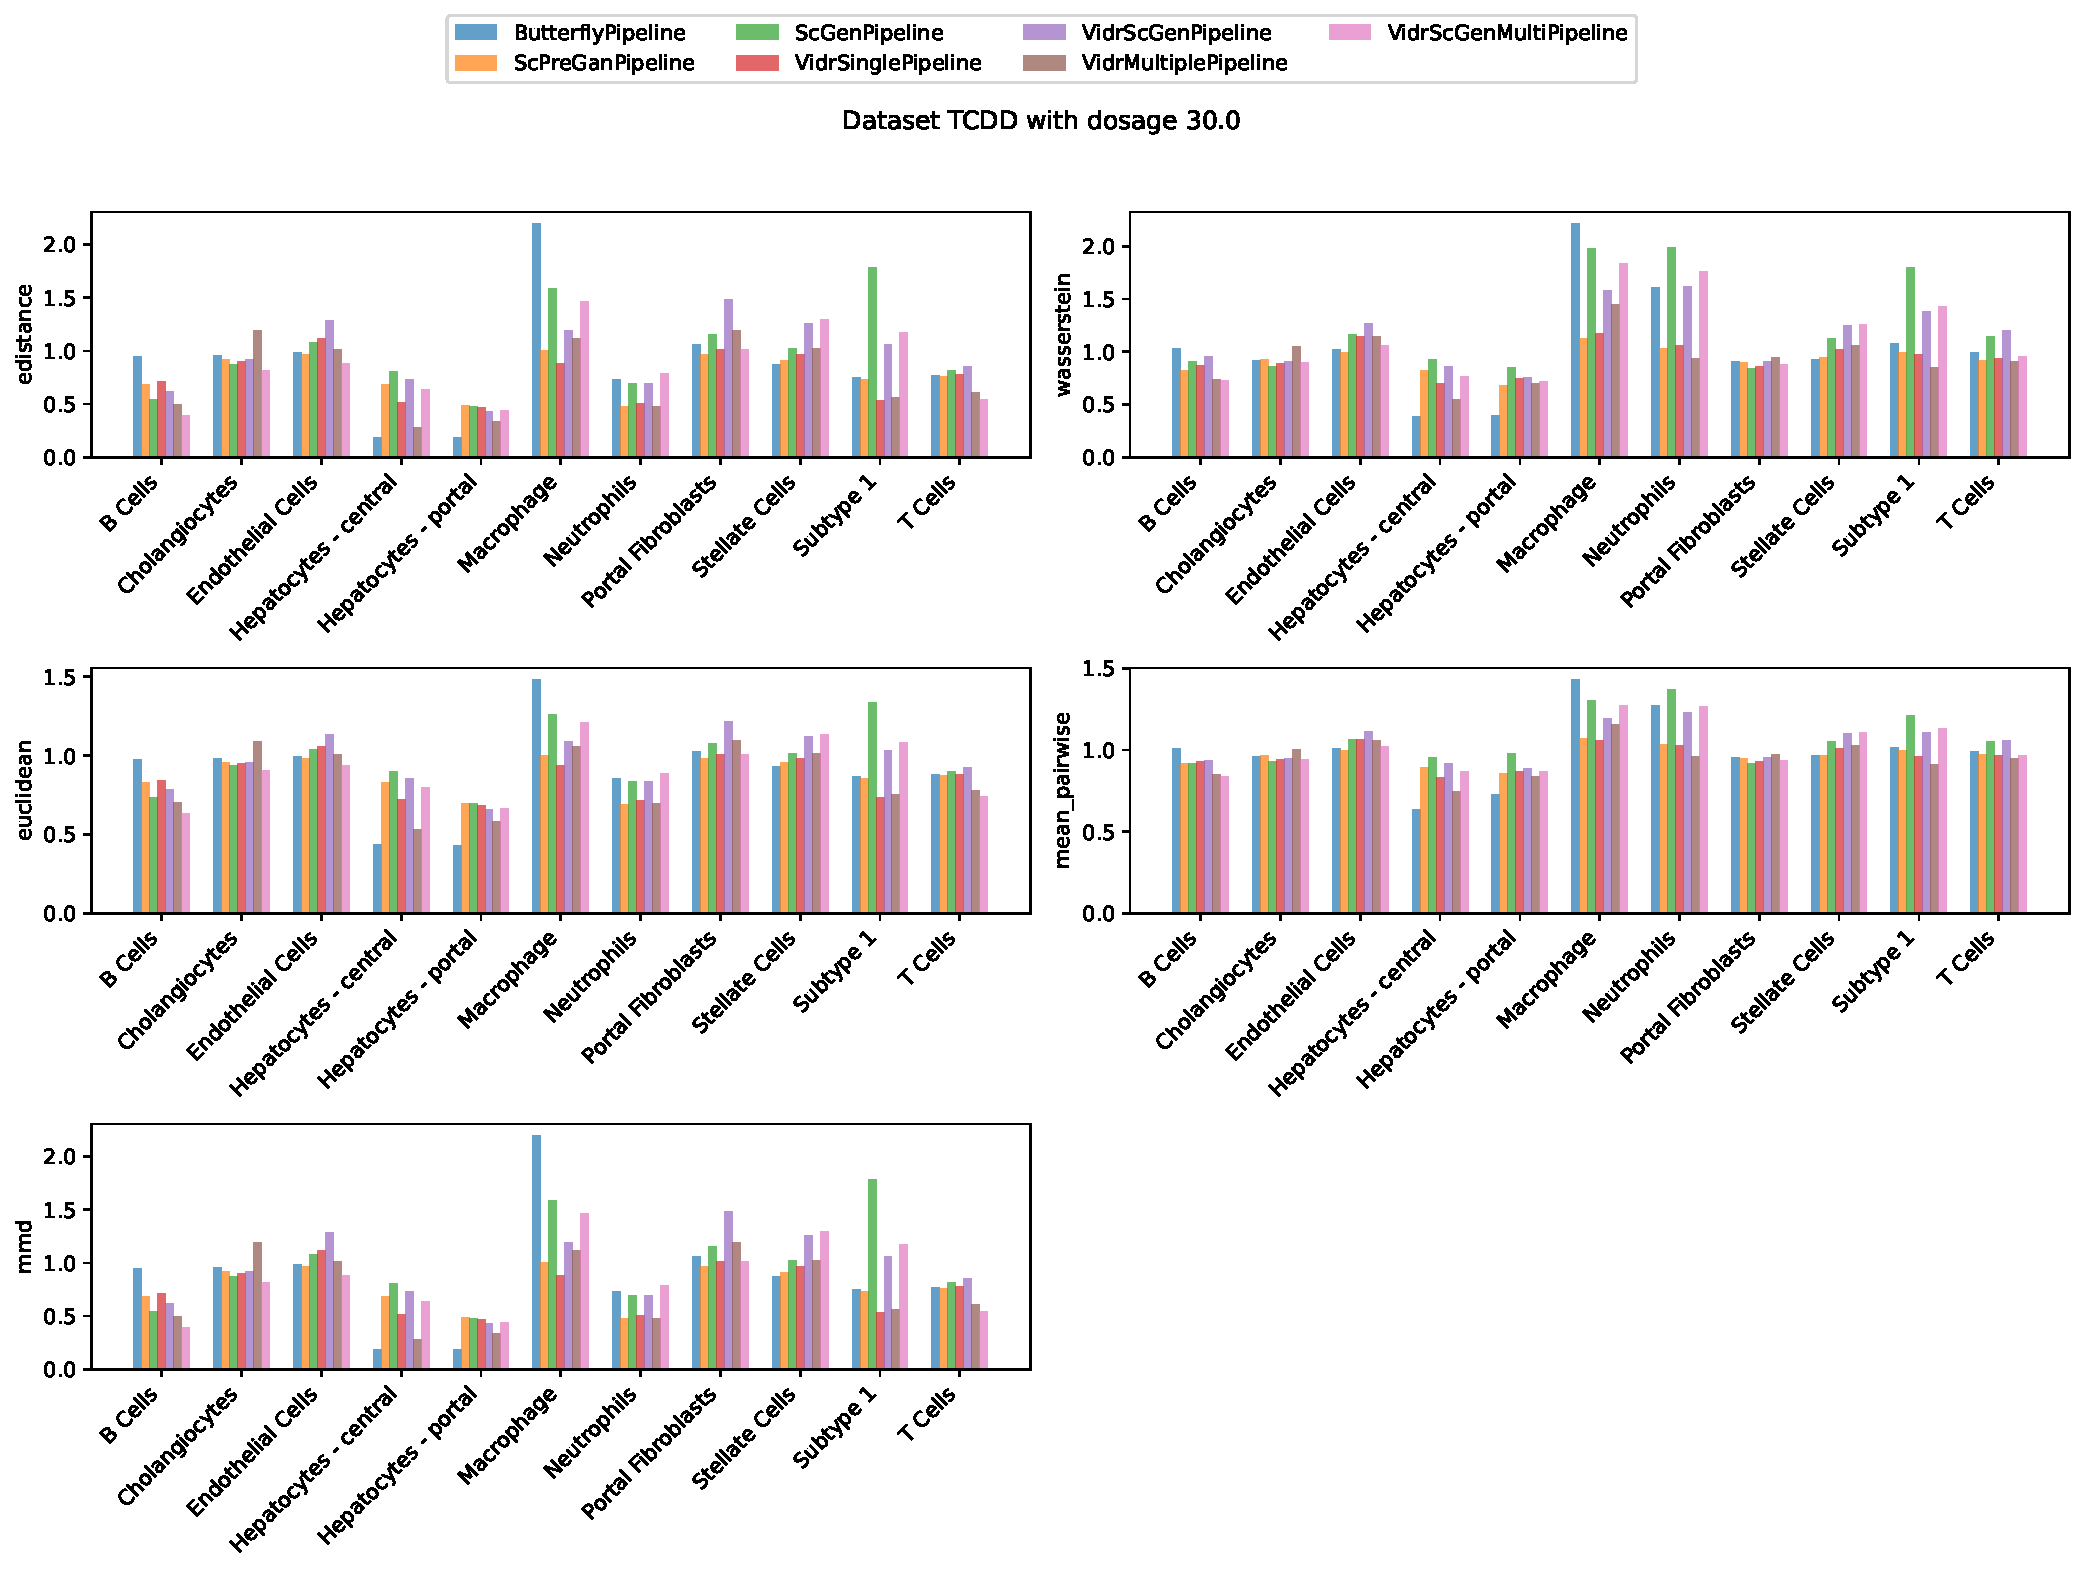
\includegraphics[width=.8\textwidth]{figures/nault_30_distance_metrics_bars.pdf}
    \caption{Distance metrics for highest dosage $30 \mu g/kg$ across cell types}
\end{figure}

\clearpage

\begin{figure}[h!]
    \centering
    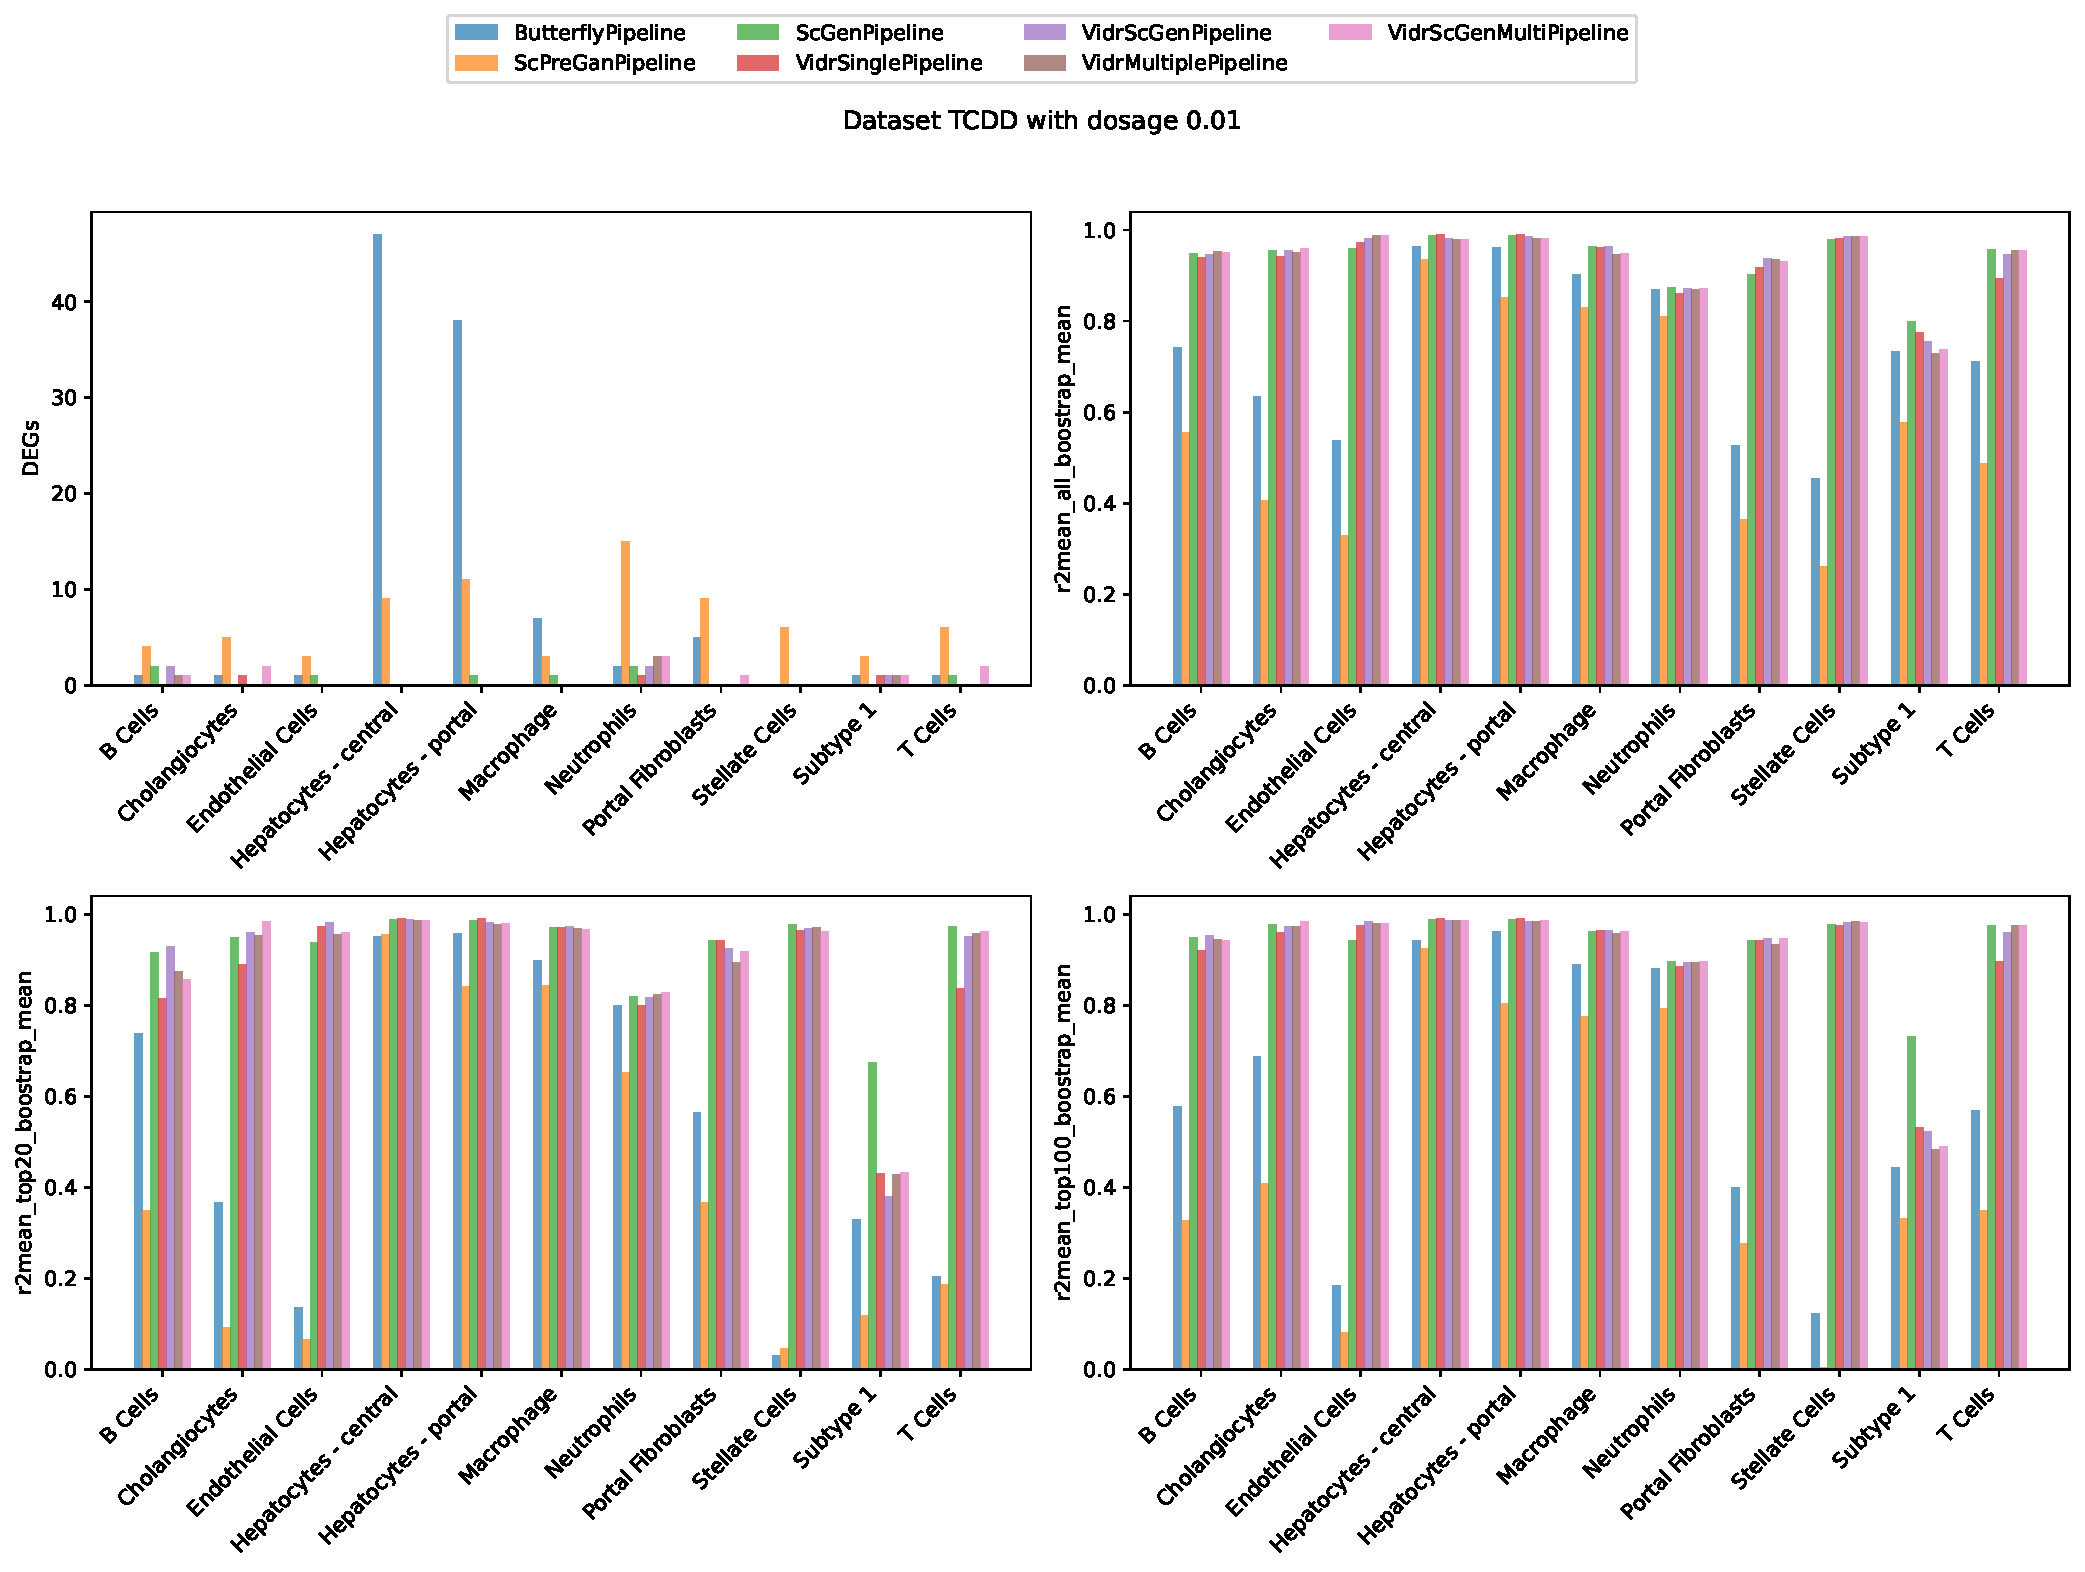
\includegraphics[width=.8\textwidth]{figures/nault_01_baseline_metrics_bars.pdf}
    \caption{Baseline metrics for lowest dosage $0.01 \mu g/kg$ across cell types}
\end{figure}

\begin{figure}[h!]
    \centering
    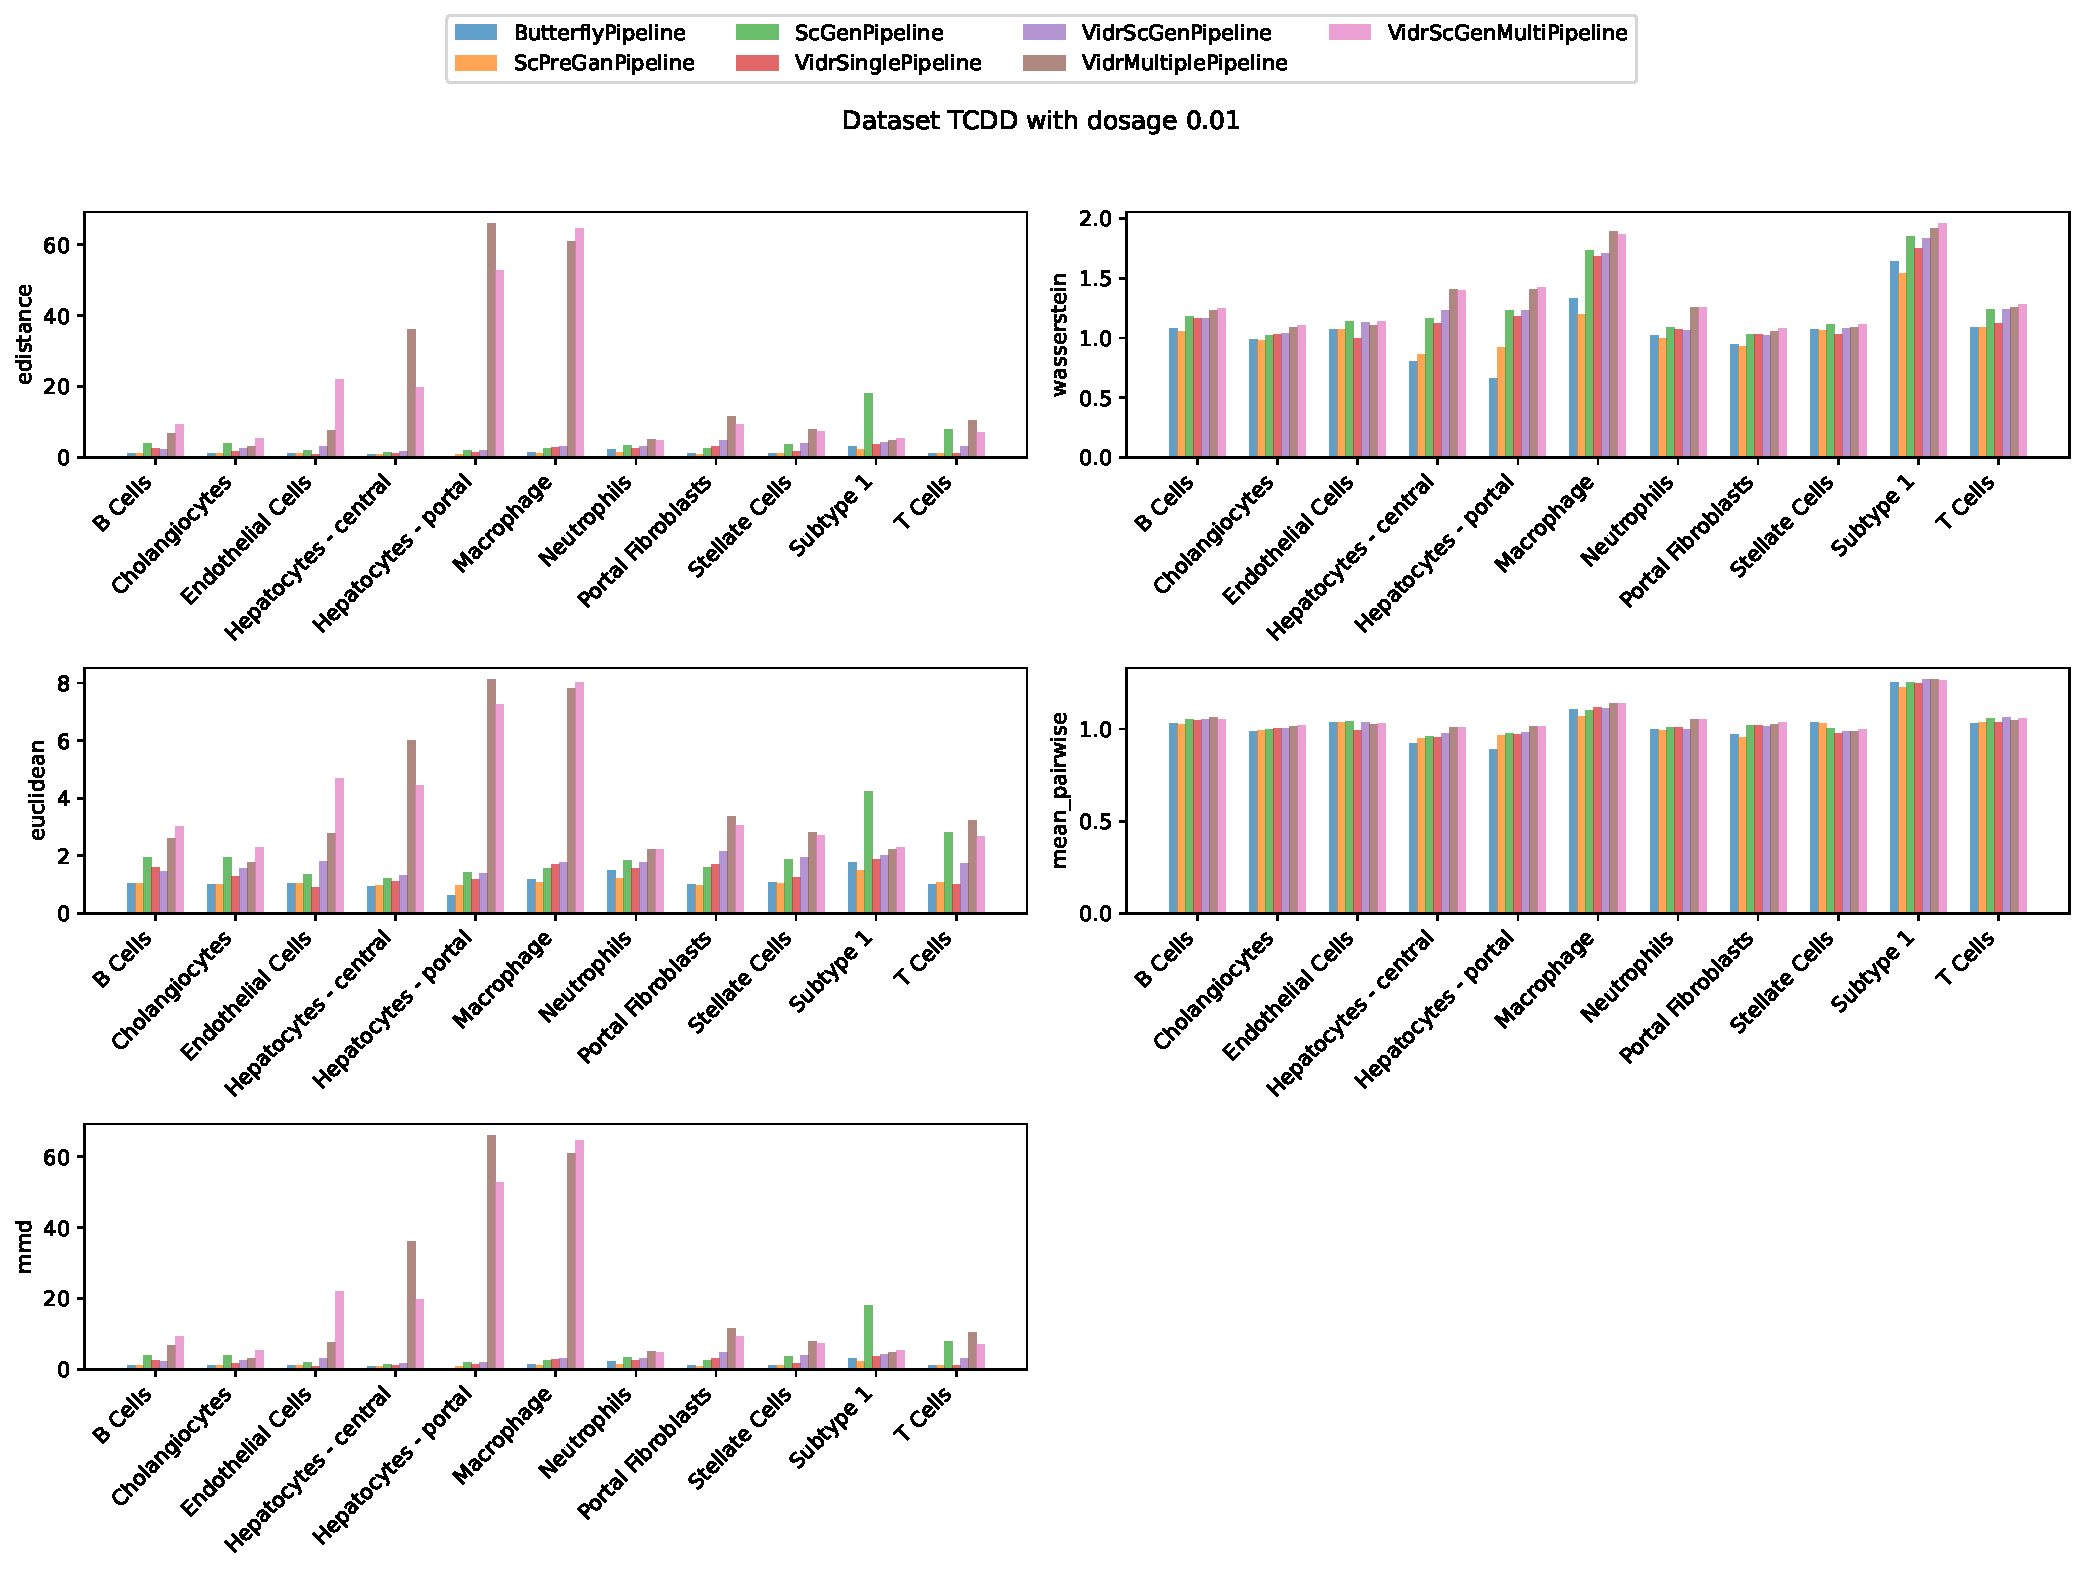
\includegraphics[width=.8\textwidth]{figures/nault_01_distance_metrics_bars.pdf}
    \caption{Distance metrics for lowest dosage $0.01 \mu g/kg$ across cell types}
\end{figure}

\clearpage


\begin{figure}[h!]
    \centering
    \includegraphics[width=.8\textwidth]{figures/nault_hepatocytes_baseline_metrics_bars.pdf}
    \caption{Baseline metrics for Hepatocytes - portal across dosages}
\end{figure}

\begin{figure}[h!]
    \centering
    \includegraphics[width=.8\textwidth]{figures/nault_hepatocytes_distance_metrics_bars.pdf}
    \caption{Distance metrics for Hepatocytes - portal across dosages}
\end{figure}

\clearpage

\begin{figure}
    \centering
    \begin{minipage}{0.49\textwidth}
        \centering
        \includegraphics[width=\textwidth]{figures/3d_nault_DEGs.pdf}
        \caption{}
    \end{minipage} \hfill
    \begin{minipage}{0.49\textwidth}
        \centering
        \includegraphics[width=\textwidth]{figures/3d_nault_r2mean_all_boostrap_mean.pdf}
        \caption{}
    \end{minipage}
    \vskip\baselineskip

    \begin{minipage}{0.49\textwidth}
        \centering
        \includegraphics[width=\textwidth]{figures/3d_nault_r2mean_top20_boostrap_mean.pdf}
        \caption{}
    \end{minipage} \hfill
    \begin{minipage}{0.49\textwidth}
        \centering
        \includegraphics[width=\textwidth]{figures/3d_nault_r2mean_top100_boostrap_mean.pdf}
        \caption{}
    \end{minipage}
    \vskip\baselineskip
\end{figure}

\clearpage

\begin{figure}
    \centering
    \begin{minipage}{0.4\textwidth}
        \centering
        \includegraphics[width=\textwidth]{figures/3d_nault_edistance.pdf}
        \caption{E-distance}
    \end{minipage} \hfill
    \begin{minipage}{0.4\textwidth}
        \centering
        \includegraphics[width=\textwidth]{figures/3d_nault_euclidean.pdf}
        \caption{Euclidean}
    \end{minipage}
    \vskip\baselineskip

    \begin{minipage}{0.4\textwidth}
        \centering
        \includegraphics[width=\textwidth]{figures/3d_nault_mean_pairwise.pdf}
        \caption{Mean pairwise}
    \end{minipage} \hfill
    \begin{minipage}{0.4\textwidth}
        \centering
        \includegraphics[width=\textwidth]{figures/3d_nault_mmd.pdf}
        \caption{MMD}
    \end{minipage}
    \vskip\baselineskip

    \begin{minipage}{0.4\textwidth}
        \centering
        \includegraphics[width=\textwidth]{figures/3d_nault_wasserstein.pdf}
        \caption{Wasserstein}
    \end{minipage}
    \caption{Distance metrics per cell type}
\end{figure}

\clearpage


\begin{figure}[h!]
    \centering
    \includegraphics[width=.9\textwidth]{figures/NaultPipeline_X_Violin_metrics0.pdf}
\end{figure}

\begin{figure}[h!]
    \centering
    \includegraphics[width=.9\textwidth]{figures/NaultPipeline_X_Violin_metrics1.pdf}
\end{figure}

\clearpage

\begin{figure}[h!]
    \centering
    \includegraphics[width=.9\textwidth]{figures/NaultPipeline_X_Boxplot_metrics0.pdf}
\end{figure}

\begin{figure}[h!]
    \centering
    \includegraphics[width=.9\textwidth]{figures/NaultPipeline_X_Boxplot_metrics1.pdf}
\end{figure}

\clearpage

\begin{figure}[h!]
    \centering
    \includegraphics[width=.9\textwidth]{figures/NaultPipeline_Y_Violin_metrics0.pdf}
\end{figure}

\begin{figure}[h!]
    \centering
    \includegraphics[width=.9\textwidth]{figures/NaultPipeline_Y_Violin_metrics1.pdf}
\end{figure}

\clearpage

\begin{figure}[h!]
    \centering
    \includegraphics[width=.9\textwidth]{figures/NaultPipeline_Y_Boxplot_metrics0.pdf}
\end{figure}

\begin{figure}[h!]
    \centering
    \includegraphics[width=.9\textwidth]{figures/NaultPipeline_Y_Boxplot_metrics1.pdf}
\end{figure}

\clearpage

\begin{figure}[h!]
    \centering
    \includegraphics[width=.8\textwidth]{figures/nault_contour_DEGs.pdf}
    \caption{DEGs}
\end{figure}

\begin{figure}[h!]
    \centering
    \includegraphics[width=.8\textwidth]{figures/nault_contour_r2mean_all_boostrap_mean.pdf}
    \caption{r2 HVGs}
\end{figure}

\clearpage

\begin{figure}[h!]
    \centering
    \includegraphics[width=.8\textwidth]{figures/nault_contour_r2mean_top20_boostrap_mean.pdf}
    \caption{r2 top 20}
\end{figure}

\begin{figure}[h!]
    \centering
    \includegraphics[width=.8\textwidth]{figures/nault_contour_r2mean_top100_boostrap_mean.pdf}
    \caption{r2 top 100}
\end{figure}

\clearpage

\begin{figure}[h!]
    \centering
    \includegraphics[width=.8\textwidth]{figures/nault_contour_edistance.pdf}
    \caption{E-distance}
\end{figure}

\begin{figure}[h!]
    \centering
    \includegraphics[width=.8\textwidth]{figures/nault_contour_euclidean.pdf}
    \caption{Euclidean}
\end{figure}

\clearpage

\begin{figure}[h!]
    \centering
    \includegraphics[width=.8\textwidth]{figures/nault_contour_mean_pairwise.pdf}
    \caption{Mean pairwise}
\end{figure}

\begin{figure}[h!]
    \centering
    \includegraphics[width=.8\textwidth]{figures/nault_contour_mmd.pdf}
    \caption{MMD}
\end{figure}

\clearpage

\begin{figure}[h!]
    \centering
    \includegraphics[width=\textwidth]{figures/nault_contour_wasserstein.pdf}
    \caption{Wasserstein}
\end{figure}

\clearpage

\section{Nault liver cell types evaluation}


\subsection{Multiple doses}


\begin{figure}[h!]
    \centering
    \includegraphics[width=.8\textwidth]{figures/nault_liver_umap_split_multiple.png}
\end{figure}

\begin{figure}[h!]
    \centering
    \includegraphics[width=.8\textwidth]{figures/nault_liver_bars_split_multiple.pdf}
\end{figure}


\subsection{Single dose 30 $\mu g/kg$}

\begin{figure}[h!]
    \centering
    \includegraphics[width=.8\textwidth]{figures/nault_liver_umap_split_30.png}
\end{figure}

\begin{figure}[h!]
    \centering
    \includegraphics[width=.8\textwidth]{figures/nault_liver_bars_split_30.pdf}
\end{figure}


\clearpage

\subsection{Comparison}


\begin{figure}[h!]
    \centering
    \includegraphics[width=.8\textwidth]{figures/nault_liver_30_baseline_metrics_bars.pdf}
    \caption{Baseline metrics for highest dosage $30 \mu g/kg$ across cell types}
\end{figure}

\begin{figure}[h!]
    \centering
    \includegraphics[width=.8\textwidth]{figures/nault_liver_30_distance_metrics_bars.pdf}
    \caption{Distance metrics for highest dosage $30 \mu g/kg$ across cell types}
\end{figure}

\clearpage

\begin{figure}[h!]
    \centering
    \includegraphics[width=.8\textwidth]{figures/nault_liver_01_baseline_metrics_bars.pdf}
    \caption{Baseline metrics for highest dosage $0.1 \mu g/kg$ across cell types}
\end{figure}

\begin{figure}[h!]
    \centering
    \includegraphics[width=.8\textwidth]{figures/nault_liver_01_distance_metrics_bars.pdf}
    \caption{Distance metrics for highest dosage $0.1 \mu g/kg$ across cell types}
\end{figure}

\clearpage

\begin{figure}[h!]
    \centering
    \includegraphics[width=.8\textwidth]{figures/nault_liver_hepatocytes_baseline_metrics_bars.pdf}
    \caption{Baseline metrics for Hepatocytes - portal across dosages}
\end{figure}

\begin{figure}[h!]
    \centering
    \includegraphics[width=.8\textwidth]{figures/nault_liver_hepatocytes_distance_metrics_bars.pdf}
    \caption{Distance metrics for Hepatocytes - portal across dosages}
\end{figure}

\clearpage


\begin{figure}
    \centering
    \begin{minipage}{0.49\textwidth}
        \centering
        \includegraphics[width=\textwidth]{figures/3d_nault_liver_DEGs.pdf}
        \caption{}
    \end{minipage} \hfill
    \begin{minipage}{0.49\textwidth}
        \centering
        \includegraphics[width=\textwidth]{figures/3d_nault_liver_r2mean_all_boostrap_mean.pdf}
        \caption{}
    \end{minipage}
    \vskip\baselineskip

    \begin{minipage}{0.49\textwidth}
        \centering
        \includegraphics[width=\textwidth]{figures/3d_nault_liver_r2mean_top20_boostrap_mean.pdf}
        \caption{}
    \end{minipage} \hfill
    \begin{minipage}{0.49\textwidth}
        \centering
        \includegraphics[width=\textwidth]{figures/3d_nault_liver_r2mean_top100_boostrap_mean.pdf}
        \caption{}
    \end{minipage}
    \vskip\baselineskip
\end{figure}

\clearpage

\begin{figure}
    \centering
    \begin{minipage}{0.4\textwidth}
        \centering
        \includegraphics[width=\textwidth]{figures/3d_nault_liver_edistance.pdf}
        \caption{E-distance}
    \end{minipage} \hfill
    \begin{minipage}{0.4\textwidth}
        \centering
        \includegraphics[width=\textwidth]{figures/3d_nault_liver_euclidean.pdf}
        \caption{Euclidean}
    \end{minipage}
    \vskip\baselineskip

    \begin{minipage}{0.4\textwidth}
        \centering
        \includegraphics[width=\textwidth]{figures/3d_nault_liver_mean_pairwise.pdf}
        \caption{Mean pairwise}
    \end{minipage} \hfill
    \begin{minipage}{0.4\textwidth}
        \centering
        \includegraphics[width=\textwidth]{figures/3d_nault_liver_mmd.pdf}
        \caption{MMD}
    \end{minipage}
    \vskip\baselineskip

    \begin{minipage}{0.4\textwidth}
        \centering
        \includegraphics[width=\textwidth]{figures/3d_nault_liver_wasserstein.pdf}
        \caption{Wasserstein}
    \end{minipage}
    \caption{Distance metrics per cell type}
\end{figure}

\clearpage


\begin{figure}[h!]
    \centering
    \includegraphics[width=.9\textwidth]{figures/NaultLiverPipeline_X_Violin_metrics0.pdf}
\end{figure}

\begin{figure}[h!]
    \centering
    \includegraphics[width=.9\textwidth]{figures/NaultLiverPipeline_X_Violin_metrics1.pdf}
\end{figure}

\clearpage

\begin{figure}[h!]
    \centering
    \includegraphics[width=.9\textwidth]{figures/NaultLiverPipeline_X_Boxplot_metrics0.pdf}
\end{figure}

\begin{figure}[h!]
    \centering
    \includegraphics[width=.9\textwidth]{figures/NaultLiverPipeline_X_Boxplot_metrics1.pdf}
\end{figure}

\clearpage

\begin{figure}[h!]
    \centering
    \includegraphics[width=.9\textwidth]{figures/NaultLiverPipeline_Y_Violin_metrics0.pdf}
\end{figure}

\begin{figure}[h!]
    \centering
    \includegraphics[width=.9\textwidth]{figures/NaultLiverPipeline_Y_Violin_metrics1.pdf}
\end{figure}

\clearpage

\begin{figure}[h!]
    \centering
    \includegraphics[width=.9\textwidth]{figures/NaultLiverPipeline_Y_Boxplot_metrics0.pdf}
\end{figure}

\begin{figure}[h!]
    \centering
    \includegraphics[width=.9\textwidth]{figures/NaultLiverPipeline_Y_Boxplot_metrics1.pdf}
\end{figure}

\clearpage

\begin{figure}[h!]
    \centering
    \includegraphics[width=.8\textwidth]{figures/nault_liver_contour_DEGs.pdf}
    \caption{DEGs}
\end{figure}

\begin{figure}[h!]
    \centering
    \includegraphics[width=.8\textwidth]{figures/nault_liver_contour_r2mean_all_boostrap_mean.pdf}
    \caption{r2 HVGs}
\end{figure}

\clearpage

\begin{figure}[h!]
    \centering
    \includegraphics[width=.8\textwidth]{figures/nault_liver_contour_r2mean_top20_boostrap_mean.pdf}
    \caption{r2 top 20}
\end{figure}

\begin{figure}[h!]
    \centering
    \includegraphics[width=.8\textwidth]{figures/nault_liver_contour_r2mean_top100_boostrap_mean.pdf}
    \caption{r2 top 100}
\end{figure}

\clearpage

\begin{figure}[h!]
    \centering
    \includegraphics[width=.8\textwidth]{figures/nault_liver_contour_edistance.pdf}
    \caption{E-distance}
\end{figure}

\begin{figure}[h!]
    \centering
    \includegraphics[width=.8\textwidth]{figures/nault_liver_contour_euclidean.pdf}
\end{figure}

\clearpage

\begin{figure}[h!]
    \centering
    \includegraphics[width=.8\textwidth]{figures/nault_liver_contour_mean_pairwise.pdf}
    \caption{Mean pairwise}
\end{figure}

\begin{figure}[h!]
    \centering
    \includegraphics[width=.8\textwidth]{figures/nault_liver_contour_mmd.pdf}
    \caption{MMD}
\end{figure}

\clearpage

\begin{figure}[h!]
    \centering
    \includegraphics[width=\textwidth]{figures/nault_liver_contour_wasserstein.pdf}
    \caption{Wasserstein}
\end{figure}

\clearpage

\subsection{Παρατηρήσεις}

\begin{itemize}
    \itemsep -0.2em
    \item Το scButterfly και το scPreGan έχουν παρόμοια συμπεριφορά στις μετρικές και εμφανίζουν μεγάλη διακύμανση κατά μήκος των τύπων των κυττάρων και των δόσεων.
    \item Τα μοντέλα που έχουν ως βάση την αρχιτεκτονική του scGen (scVIDR, και οι παραλλαγές του), VAR και post-processing στο latent space, έχουν την υψηλότερη και πιο σταθερή απόδοση σε μετρικές του $R^2$, ωστόσο υστερούν στην καταμέτρηση των κοινών διαφοροποιήσιμων γονιδίων έκφρασης (DEGs).
\end{itemize}

\clearpage

\section{PBMC}


\begin{figure}[h!]
    \centering
    \includegraphics[width=.8\textwidth]{figures/pbmc_split.png}
\end{figure}

\begin{figure}[h!]
    \centering
    \includegraphics[width=.8\textwidth]{figures/pbmc_bars_split.pdf}
\end{figure}

\clearpage

\subsection{Comparison}

\begin{figure}[h!]
    \centering
    \includegraphics[width=.8\textwidth]{figures/pbmc_baseline_metrics_bars.pdf}
\end{figure}

\begin{figure}[h!]
    \centering
    \includegraphics[width=.8\textwidth]{figures/pbmc_distance_metrics_bars.pdf}
\end{figure}